%\documentclass[draftfoot,12pt]{cit_thesis}
\documentclass[12pt]{caltech_thesis}
\usepackage{feynmp}
\unitlength=1mm 
\DeclareGraphicsRule{.1}{mps}{*}{}
\DeclareGraphicsRule{.2}{mps}{*}{}
\DeclareGraphicsRule{.3}{mps}{*}{}
\DeclareGraphicsRule{.4}{mps}{*}{}
\DeclareGraphicsRule{.5}{mps}{*}{}
\DeclareGraphicsRule{.6}{mps}{*}{}
\usepackage{pennames}
\usepackage{ptdr-definitions}
\usepackage{multirow}
\usepackage{amsmath}
\usepackage{amsthm} % Theorem Formatting
\usepackage{amssymb}	% Math symbols such as \mathbb
\usepackage{mathrsfs}
\newlength\cmsFigWidth
\setlength\cmsFigWidth{0.85\columnwidth}
\newcommand{\cmsLeft}{top}
\newcommand{\cmsRight}{bottom}
\newcommand{\CL}{C.L.\xspace}
\newcommand{\cmsUpperLeft}{top}
\newcommand{\cmsUpperRight}{middle}
\newcommand{\CLs}{\ensuremath{\mathrm{CL}_\mathrm{s}}\xspace}
\newcommand{\MR}{\ensuremath{M_\mathrm{R}}\xspace}
\newcommand{\MRz}{\ensuremath{M_\mathrm{R}^0}\xspace}
\newcommand{\Rtwo}{\ensuremath{\mathrm{R}^2}\xspace}
\newcommand{\Rtwoz}{\ensuremath{\mathrm{R}^2_0}\xspace}
\newcommand{\R}{\ensuremath{\mathrm{R}}\xspace}
\newcommand{\MRT}{\ensuremath{M_\mathrm{T}^\mathrm{R}}\xspace}
\providecommand{\cPV}{\ensuremath{\cmsSymbolFace{V}}\xspace}

\usepackage{tikz}
\usepackage{ifthen}
\usetikzlibrary{fadings}
\definecolor{x0p00y0p00}{rgb}{0.6,1,0.18}
\definecolor{x1p00y0p00}{rgb}{0,0,1}
\definecolor{x0p00y1p00}{rgb}{1,0,0}
\definecolor{x0p50y0p00}{rgb}{0,0.5,0.6}
\definecolor{x0p00y0p50}{rgb}{1,0.5,0}
\definecolor{x0p50y0p50}{rgb}{0.6,0,0.6}
\definecolor{x0p25y0p25}{rgb}{0.6,0.6,0.6}
\definecolor{x0p25y0p50}{rgb}{0.8,0.7,0.6}
\definecolor{x0p50y0p25}{rgb}{0.6,0.7,0.8}

\usepackage{palatino}%    Choose default roman font.  Others are times, pslatex, newcent, bookman, chancery
\usepackage{mathpazo}%  Matching math fonts (see http://www.math.uiuc.edu/~hartke/computer/latex/survey/survey.html)
\usepackage{helvet}%      Choose default sans serif
%\usepackage{sectsty}%     Change style of headings (should precede section redefinitions below)
%\allsectionsfont{\sffamily}% Set sans serif for all headings

\usepackage[hyphens]{url}
\usepackage[colorlinks=true,linktocpage=true,urlcolor=blue,linkcolor=blue,citecolor=purple]{hyperref}
\usepackage{lipsum}
\usepackage{graphicx}

\usepackage{todonotes}

% Must use biblatex to produce the Published Contents and Contributions, per-chapter bibliography (if desired), etc.
\usepackage[
    backend=biber,natbib,
    style=numeric
]{biblatex}

% Name of your .bib file(s)
\addbibresource{duarte_thesis.bib}

\begin{document}
\author{Javier M. G. Duarte}
\title{Naturalness Confronts Nature: Searches for Supersymmetry with
  the CMS Detector}


\degreeaward{Doctor of Philosophy}                 % Degree to be awarded
\university{California Institute of Technology}    % Institution name
\address{Pasadena, California}                     % Institution address
\unilogo{caltech.png}                                 % Institution logo
\copyyear{2016}  % Year (of graduation) on diploma
\defenddate{August 11, 2016}          % Date of defense

\orcid{0000-0002-5076-7096}

\rightsstatement{All rights reserved.}

\maketitle[logo]                  % title page and (if not a technical
                            % report)                                                                                           
\begin{dedication}          % optional dedication                                                                                                                   
To my mother and my sister.
\end{dedication}

\begin{acknowledgments}     % optional acknowledgments      
                                                                                                         
First, I thank my advisor Maria Spiropulu. Her
wisdom, experience, and warmth have shaped me as I've
developed as a scientist. For her endless contributions to my life
and career, I am in her debt.

I thank Maurizio Pierini for his intense mentorship beginning at CERN
in 2011 and continuing to this day. Maurizio taught me how to be a
modern particle physicist, by sharing his expertise in computing, statistics, and
phenomenology. He was also invaluable in helping me prepare this manuscript.

I also thank Chris Rogan for guiding me during my first days of
graduate school and for being a good friend. Cristi\'{a}n Pe\~{n}a and
Dustin Anderson have been constant friends and fellow soldiers in
graduate school. I thank my other colleagues in the Caltech CMS group
for their help and advice during graduate school: Si Xie, Artur
Apresyan, Jean-Roch Vlimant, and Adi Bornheim.

I thank my roommates and close friends: Ingmar Saberi, Tristan McKinney,
Eric Quintero, and Evelyn Gomez. They continually inspire me and
remind me to have fun every once in a while. 
I also thank the other two legs of our marathon running team, Alex Tuna and Phil Hebda, for their friendship,
which has spanned many years and two continents, and for constantly challenging
me to improve my marathon PR.

I dedicate this thesis to my mother, Bruny, and my sister, Rossy, for
loving and supporting me throughout my life.

Finally, I thank my girlfriend Kristen Jezior. Without her love,
kindness, and humor, I would be lost.

\end{acknowledgments}
\begin{abstract}
In this thesis, we present two inclusive searches for supersymmetric
particles at $\sqrt{s}=8\TeV$ and $13\TeV$ using the razor variables and guided
by the principle of naturalness. We build a framework to explore the
natural supersymmetry parameter space of gluino and top squark masses
and branching ratios, which represents a unique attempt to cover this
parameter space in a more complete way than ever before. With this approach, the production of top squarks and
gluinos are excluded below $\sim700\TeV$ and $\sim1.6\TeV$, respectively,
independent of the branching ratios. We also propose alternative simplified models to study
$\PH+\mathrm{jet}$ events at the LHC, and reinterpret an excess
observed at $8\TeV$ in the context of these models. Motivated by the
need to mitigate the effects of multiple interactions per bunch
crossing (pileup), an essential feature of present and future
colliders, we study the precision timing capabilities of a LYSO-based sampling calorimeter, and achieve a time
resolution of $\sim30\unit{ps}$ in electron test beam measurements. The
achieved resolution corresponds to the precision needed to significantly reduce the inclusion of pileup particles in the
reconstruction of the event of interest. We discuss a search for narrow resonances
in the dijet mass spectrum at $13\TeV$ using the data-scouting
technique at CMS, which records a smaller event format to increase the
maximum recordable rate. For the benchmark models with a vector or axial-vector
mediator that couples to quarks and dark matter particles, the dijet
search is more sensitive and excludes a larger range of
($m_{\mathrm{med}}$,$m_{\mathrm{DM}}$) parameter space than traditional $\MET+\mathrm{X}$ searches at the LHC.
\end{abstract}


\tableofcontents
\listoffigures
\listoftables
\printnomenclature

\mainmatter

\chapter{Introduction}
\label{ch:intro}

The standard model (SM) of particle physics is a description of nature
composed of two main ingredients:
\begin{enumerate}[(a)]
\item a list of known particles and their quantum properties, and
\item an inventory of the interactions of these particles through the fundamental forces
(except for gravity): the strong nuclear force, the weak nuclear force, and the electromagnetic
force. 
\end{enumerate}
The discovery of the Higgs boson, announced by the CMS and ATLAS
collaborations on July 4, 2012~\cite{CMShiggs,ATLAShiggs}, was
thought to be the final missing piece that completes and confirms the
SM as a description of nature. However, several theoretically- and
experimentally-motivated questions remain unanswered. Three
of the most important questions are:
\begin{enumerate}[(a)]
\item What is the origin of \emph{dark matter} whose existence is
  inferred from measurements of galactic rotation curves~\cite{1980ApJrotationcurves,1989HIrotationcurves} and weak gravitational lensing
  observations of the ``Bullet cluster''~\cite{Clowe:2006eq}?
\item Do the strong nuclear, weak nuclear, and electromagnetic
  forces unify at a high energy scale?
\item How does a fundamental scalar like the Higgs boson remain
  ``light'' when its mass is sensitive to new particles at high energy
  scales through radiative corrections?
\end{enumerate}

In the 1970s, \emph{supersymmetry} was proposed as a
possible extension of spacetime symmetry that relates fermions and
bosons~\cite{Ramond,Golfand,Volkov,Wess,Fayet}. Little
more than a mathematical curiosity at first, supersymmetry
emerged as the leading candidate for a theory of physics beyond the
standard model in the 1980s and 1990s, as it was understood that this 
principle may provide an economical and beautiful solution to
three pressing issues in the SM by (a) providing a weakly interacting particle candidate for dark
matter~\cite{Ellis:1983ew,Jungman:1995df}, (b) exhibitting gauge coupling
unification~\cite{Dimopoulos:1981yj,Marciano:1981un,Einhorn:1981sx,Ibanez:1981yh,Amaldi:1991cn,Langacker:1995fk},
and (c) alleviating the fine-tuning of the Higgs mass~\cite{Witten:1981nf,Dimopoulos:1981zb,Dine:1981za,Dimopoulos:1981au,Sakai:1981gr,Kaul:1981hi}.

This thesis focuses on efforts to discover supersymmetric
particles in collider searches and is divided into five parts. It is
the story of how we examined the principal motivation for supersymmetry,
constructed simplified model hypotheses based on this guiding
principle, and exhaustively searched the supersymmetric phase space
using an optimal basis of observables, known as the \emph{razor variables}.

In Part~\ref{part:intro}, the SM, supersymmetry, and naturalness are
introduced, motivating the search for natural SUSY. The razor approach
to supersymmetric kinematics is detailed in
Sec.~\ref{sec:kinematic}. Part~\ref{part:searches} begins with a description of the CMS
experiment and the LHC. Chapters~\ref{ch:analysis8TeV}~and~\ref{ch:analysis13TeV} present
two searches for natural SUSY performed at $\sqrt{s}=8
\TeV$ and $13 \TeV$, which together represent a unique attempt to cover the phase space of
natural SUSY in a more complete way than ever before. Finally,
Chapter~\ref{ch:pheno} studies an excess observed in data at $\sqrt{s}=8
\TeV$ and proposes alternative simplified natural SUSY models to study
at $\sqrt{s}=13 \TeV$. 

Part~\ref{part:timing} motivates probing the \TeV and multi-\TeV scale
with high-luminosity colliders as ``the final hiding place'' of
natural SUSY. Chapter~\ref{ch:timing} discusses the
requirements for detectors at future high-luminosity colliders,
specifically the need for calorimeters with precision
timing capabilities due to the high rate of simultaneous interactions
per bunch crossing (pileup) anticipated. Finally, we present a
proof-of-concept LYSO-based sampling calorimeter, and estimate its
ultimate timing performance capability based on test-beam
measurements.

Although not the main focus of this thesis, Part~\ref{part:app}
describes an important search for exotic new physics in the dijet mass
spectrum at $\sqrt{s}=13 \TeV$. Partially motivated by
the excess at $750 \GeV$ in both the CMS and ATLAS diphoton mass
spectra, the search extends the previous dijet searches by searching
in the low-mass end of the spectrum ($>450 \GeV$) using the
CMS data scouting technique.
\section{The Standard Model of Particle Physics}

The standard model (SM) of particle physics describes all of the known
particles and their interactions through the fundamental forces
(except for gravity): the strong nuclear force, the weak nuclear force, and the electromagnetic
force. These forces arise due to the exchange of spin-$1$
bosons among the spin-$\frac{1}{2}$ fermions that make up matter. The SM is a renormalizable quantum field
theory based on the gauge symmetry group $\mathrm{SU(3)}_{\mathrm{C}}\times \mathrm{SU(2)}_{\mathrm{L}}\times
\mathrm{U(1)}_Y$. Each factor in the gauge group corresponds to a fundamental force, represented by a gauge field, whose excitations are
the gauge bosons that act as force carriers:
\begin{center}
\begin{tabular}{ccccc}
$\mathrm{SU(3)}_{\mathrm{C}}$ &$\times$& $\mathrm{SU(2)}_{\mathrm{L}}$
  &$\times$& $\mathrm{U(1)}_Y$\\
 $\downarrow$&&$\downarrow$&&$\downarrow$\\
 $G_{\mu}^{\alpha}$&&$W^a_{\mu}$&&$B_{\mu}$\\
 $\alpha=1,...,8$&&$a=1,2,3$&&
\end{tabular}
\end{center}
The eight spin-$1$ bosons, $G_{\mu}^{\alpha}$,
associated with the factor $\mathrm{SU(3)}_{\mathrm{C}}$ are the gluons. Any
particle that transforms is said to carry color charge. The three spin-$1$
bosons, $W^{a}_{\mu}$ are associated 

The matter fields are fermions, which fall into two
categories: the quarks, $u$, $d$, $c$, $s$, $t$, and $b$, which participate in the
strong interactions, and the leptons, $e$, $\mu$, $\tau$, $\nu_e$,
$\nu_{\mu}$, and $\nu_{\tau}$, which do
not. Fig.~\ref{fig:standardmodel} shows the particles in the SM. To simplify notation, it makes sense to consider the doublet of
$q_L = \binom{u_L}{d_L}$ and $\ell_L = \binom{e_L}{\nu_L}$. All matter fields implicity have
three-component generation indices $e_i=(e,\mu,\tau),
\nu_i=(\nu_e,\nu_{\mu},\nu_{\tau}), u_i=(u,c,t),
d_i=(d,s,b)$. 

The electric charge is given by $Q = T_{3L}+Y$. Tab.~\ref{tab:representations} summarizes the
representations in which the fields transform under the SM
gauge group. The SM Langrangian
excluding Higgs and Yukawa terms is then,
\begin{align}
\mathcal{L}_{\mathrm{SM}} &= -\frac{1}{4}B_{\mu\nu}B^{\mu\nu} -\frac{1}{4}W^{a}_{\mu\nu}W^{a\mu\nu} - \frac{1}{4}G^{\alpha}_{\mu\nu}G^{\alpha\mu\nu}
  & \mathrm{(gauge~terms)}\nonumber\\
& +\bar\ell_L\tilde\sigma^{\mu}iD_{\mu}\ell_L +
   \bar e_R\sigma^{\mu}iD_{\mu}e_R + \bar v_R
   \sigma^{\mu}iD_{\mu}\nu_R + (\mathrm{h.c.})& \mathrm{(lepton~kinetic~terms)}\nonumber\\
& +\bar q_L\tilde\sigma^{\mu}iD_{\mu}q_L +
   \bar u_R\sigma^{\mu}iD_{\mu}u_R + \bar d_R
   \sigma^{\mu}iD_{\mu}d_R + (\mathrm{h.c.})& \mathrm{(quark~kinetic~terms)}\nonumber\\
& +\mathcal L_{\mathrm{Higgs}} +\mathcal L_{\mathrm{Yukawa}} &  \mathrm{(Higgs~and~Yukawa~terms)}
\label{eqn:lsm}
\end{align}
where $D_{\mu}$ is the gauge covariant derivative.

\begin{figure}
\centering
\includegraphics[width=0.7\textwidth]{figs/theory/standardmodel.pdf}
\caption{\label{fig:standardmodel} The particles in the standard model.}
\end{figure}

\begin{table}
\centering
\begin{tabular}{c|ccc}
&$\mathrm{SU(3)}_{\mathrm{C}}$&$\mathrm{SU(2)}_{\mathrm{L}}$&$\mathrm{U(1)}_Y$ \\
$q$ & $\mathbf{3}$ & $\mathbf{2}$ & $1/6$\\
$\bar u_R$ & $\mathbf{\bar 3}$ & $\mathbf{1}$ & $-2/3$\\
$\bar d_R$ & $\mathbf{\bar 3}$ & $\mathbf{1}$ & $1/3$\\
$\ell$ & $\mathbf{1}$ & $\mathbf{2}$ & $-1/2$\\
$\bar e_R$ & $\mathbf{1}$ & $\mathbf{1}$ & $1$\\\hline
$h$ & $\mathbf{1}$ & $\mathbf{2}$ & $1/2$
\end{tabular}
\caption{\label{tab:representations} Table summarizing the
    representations in which the fields transform under the standard
    model gauge group.}
\end{table}


\section{Electroweak Symmetry Breaking}
A central feature of gauge theories is that the gauge bosons are
massless due to the fact that the gauge symmetry forbids explicit mass
terms in the Lagrangian. In 1964, it was proposed that spontaneous symmetry breaking in gauge
theories could be achieved through the introduction of a scalar
field~\cite{PhysRevLett.13.321,HIGGS1964132,PhysRevLett.13.508,PhysRevLett.13.585,PhysRev.145.1156,PhysRev.155.1554}. In
the SM, the mechanism of electroweak symmetry breaking
is a framework to keep the structure of gauge symmetry and
interactions at high energy, and still generate the observed masses
of the $\PW$ and $\PZ$ gauge
bosons~\cite{PhysRevLett.19.1264,GLASHOW1961579,Salam:1968rm}. The SM
Higgs part of the Lagrangian is: 
\begin{align}
\mathcal L_{\mathrm{Higgs}} &= (D_{\mu}\Phi)^{\dagger}(D^{\mu}\Phi) -
V(\Phi)~;& V(\Phi) &= -\mu^2\Phi^{\dagger}\Phi +
\lambda(\Phi^{\dagger}\Phi)^2~,
\label{eqn:Lhiggs}
\end{align}
where the field $\Phi$ is a self-interacting
$\mathrm{SU(2)}_{\mathrm{L}}$ complex doublet with weak hypercharge $Y=1/2$:
\begin{equation}
\Phi = \left(\begin{matrix} \phi^{+}\\\phi^0\end{matrix} \right)~.
\end{equation}
If the quadratic term is negative, that is $\mu^2>0$, then the
potential will have a ``Mexican hat'' shape, illustrated in
\ref{fig:mexicanhat}, and the minimum of the potential will occur at a value of the field that is not $\mathrm{SU(2)}_{\mathrm{L}}\times\mathrm{U(1)}_Y$
invariant. Due to this, the complex scalar doublet field acquires a nonzero vacuum
expectation value (\emph{vev}), corresponding to the minimum of the potential,
\begin{align}
\langle\Phi\rangle_0&\equiv \langle 0|\Phi|0\rangle =
\frac{1}{\sqrt{2}}U(x)\left(\begin{matrix} 0\\v\end{matrix} \right)~;&v &= \sqrt{\frac{\mu^2}{\lambda}};
\end{align}
where $U(x)$ is a unitary transformation that rotates the field
to the other degenerate solutions. Since the vev is still symmetric under a $\mathrm{U(1)}$ subgroup of the full
electroweak symmetry, we say the electroweak symmetry
$\mathrm{SU(2)}_{\mathrm{L}}\times\mathrm{U(1)}_Y$ is \emph{spontaneously
broken} to $\mathrm{U(1)}_{\mathrm{EM}}$. Spontaneous symmetry breaking
is the phenomenon in which the equations of the dynamics are
exactly symmetric, but they admit solutions that are not.

\begin{figure}
\centering
\includegraphics[width=0.7\textwidth]{figs/theory/MexicanHat.pdf}
\caption{\label{fig:mexicanhat} The shape of the ``mexican hat''
  potential. The minimum of the potential occurs at
a field value that is not 0.}
\end{figure}

This mechanism is responsible for generating the masses of the gauge
bosons in the standard model, as can be seen by evaluating the 
covariant derivative in Eqn.~\ref{eqn:Lhiggs},
\begin{equation}
D_{\mu}\Phi = (\partial_{\mu} - i g_2 \frac{\sigma_a}{2}W^a_{\mu} -
ig_1\frac{1}{2}B_{\mu})\Phi ~,
\end{equation}
on the vacuum Higgs field. In this case, the kinetic term is:
\begin{align}
|D_{\mu}\Phi|^2 &= \frac{1}{2} \left|\left (\begin{matrix}\partial_{\mu}
    -\frac{i}{2}(g_2W_{\mu}^3 + g_1B_{\mu})&
    -\frac{ig_2}{2}(W_{\mu}^1-iW_{\mu}^2)\\ 
-\frac{ig_2}{2}(W_{\mu}^1+iW^2_{\mu})&\partial_{\mu}
    +\frac{i}{2}(g_2W_{\mu}^3 - g_1B_{\mu})
  \end{matrix}\right)
                                       \left(\begin{matrix}0\\v\end{matrix}\right)\right |^2 \nonumber\\
& = \frac{1}{8} \left ( g_2^2v^2|W_{\mu}^1+iW^2_{\mu}|^2 +
  v^2|g_2W^3_{\mu}-g_1B_{\mu}|^2 \right ) \nonumber\\
& = m_W^2W_{\mu}^+W^{-\mu} +
\frac{1}{2}m_Z^2Z_{\mu}Z^{\mu}~ + \frac{1}{2}m_{\gamma}^2A_{\mu}A^{\mu},
\end{align}
where we can identify three field combinations, $W_{\mu}^{\pm}$ and
$Z_{\mu}$, which have bilinear mass terms, and a fourth $A_{\mu}$,
which does not:
\begin{align}
W_{\mu}^{\pm} &= \frac{1}{\sqrt{2}}(W_{\mu}^1\mp iW^2_{\mu})~, &m_W &= \frac{1}{2}vg_2~,\\
Z_{\mu} &= \frac{g_2W_{\mu}^3 - g_1B_{\mu}}{\sqrt{g_1^2+g_2^2}}~,&m_Z &= \frac{1}{2}v\sqrt{g_1^2+g_1^2}~,\\
A_{\mu} &= \frac{g_2W_{\mu}^3 + g_1B_{\mu}}{\sqrt{g_1^2+g_2^2}}~,&m_{\gamma} &= 0.
\end{align}
The $\PW$ and $\PZ$ bosons have acquired mass, while the photon
$\Pgg$ remains massless.

Another consequence of this symmetry breaking mechanism is the
emergence of a physical scalar boson. If we expand the field around
its potential minimum
\begin{align}
\Phi(x)&=
\frac{1}{\sqrt{2}}U(x)\left(\begin{matrix} 0\\v+H(x)\end{matrix} \right)
\end{align}
and write out the terms associated to this field, we find
\begin{equation}
\mathcal L_{\mathrm{Higgs}} \supset \frac{1}{2}(\partial^{\mu}H)^2 -
\lambda v^2 H^2 - \lambda v H^3 - \frac{\lambda}{4}H^4~.
\end{equation}
which means this scalar boson, called the \emph{Higgs boson}, is self-interacting and has a mass squared of $m^2_{h^0} =
2\lambda v^2$ at tree-level.

\subsection{Fermion Masses}
As proposed by Weinberg~\cite{PhysRevLett.19.1264}, fermions acquire
mass through interaction with the $\Phi$ field, which has a nonzero
vev. This is accomplished by adding Yukawa terms to the Lagrangian for
each generation,
\begin{equation}
\mathcal L_{\mathrm{Yukawa}} = - \lambda_e \bar\ell_L\Phi e_R -
\lambda_u\bar q_L\Phi u_R  - \lambda_d\bar q_L\tilde\Phi d_R + (\mathrm{h.c.})~,
\end{equation}
where the doublet $\tilde\Phi = i\sigma_2\Phi^{\ast}$ with hypercharge $Y=-1/2$ is
needed to generate masses for the down-type quarks. Then we can
identify the fermion masses as
\begin{align}
m_e &= \frac{\lambda_e v}{2}&m_u &= \frac{\lambda_e
                                          v}{2}& m_d &= \frac{\lambda_dv}{2}~.
\end{align}
Neutrino masses can also be accommodated in the SM by adding similar terms.


\section{Higgs Mass and Naturalness}
The leading quantum correction to the Higgs mass squared parameter is due to
the large Yukawa coupling coupling to the top quark, which gives the
top quark its large mass,
\begin{fmffile}{higgs}
\begin{align}
\Delta(m^2_{h^0}) &= \quad\parbox{20mm}{
\begin{fmfgraph*}(20,20)
\fmfkeep{fermion}
\fmfleft{i} 
\fmfright{o} 
\fmf{dashes}{i,v1}
\fmf{dashes}{v2,o}
\fmf{plain,left,tension=.3,label=$t$}{v1,v2}
\fmf{plain,left,tension=.3}{v2,v1}
\fmfv{label=$h^0$,label.angle=90}{i}
\end{fmfgraph*}} \quad + \quad\cdots\\
&= -\frac{|\lambda_t|^2}{8\pi^2}\Lambda_{\mathrm{UV}}^2 + \cdots~,
\end{align}
where $\Lambda_{\mathrm{UV}}$ is an ultraviolet momentum cutoff. This
quadratic dependence on the $\Lambda_{\mathrm{UV}}$ means the Higgs
mass parameter is sensitive to the physics in the
ultraviolet. This sensitivity requires a large fine tuning to explain
why $m^2_{h^0}$ remains small.

\begin{align}
\Delta(m^2_{h^0}) &= \quad\parbox{20mm}{\fmfreuse{fermion}} \quad + \quad
\parbox{20mm}{
\begin{fmfgraph*}(20,20)
\fmfkeep{boson}
\fmfleft{i} 
\fmfright{o} 
\fmf{dashes}{i,v}
\fmf{dashes,right,tension=0.7,label=$\tilde t_{1,,2}$}{v,v}
\fmf{dashes}{v,o}
\fmfv{label=$h^0$,label.angle=90}{i}
\end{fmfgraph*}}
 \quad + \quad
\parbox{20mm}{
\begin{fmfgraph*}(20,20)
\fmfkeep{sunset}
\fmfleft{i}
\fmfright{o}
\fmf{dashes}{i,v1}
\fmf{dashes}{v2,o}
\fmf{dashes,left,tension=.3,label=$\tilde t_{1,,2}$}{v1,v2}
\fmf{dashes,left,tension=.3}{v2,v1}
\fmfv{label=$h^0$,label.angle=90}{i}
\end{fmfgraph*}} \quad + \quad\cdots\\
 &= -\frac{|\lambda_t|^2}{8\pi^2}\Lambda_{\mathrm{UV}}^2 +
  \sum_{i=1}^{2} \left ( \frac{\lambda_{\tilde
  t_i}^2}{16\pi^2}\Lambda_{\mathrm{UV}}^2 - 2m_{\tilde
  t_i}^2\log(\Lambda_{\mathrm{UV}}/m_{\tilde t_i}) \right )+ \cdots~,
\end{align}
\end{fmffile}

\section{Supersymmetry}
Supersymmetry (SUSY) is a proposed symmetry of spacetime that 
introduces a bosonic (fermionic) partner for every fermion (boson) in the 
standard model
(SM)~\cite{Wess,Golfand,Volkov,Chamseddine,Kane,Fayet,Barbieri,Hall,Ramond}.

Supersymmetric extensions of the SM are particularly compelling 
because they yield solutions to the gauge hierarchy problem with no
fine-tuning of fundamental parameters~\cite{Witten:1981nf,Dimopoulos:1981zb,Dine:1981za,Dimopoulos:1981au,Sakai:1981gr,Kaul:1981hi}, 
exhibit gauge coupling unification~\cite{Dimopoulos:1981yj,Marciano:1981un,Einhorn:1981sx,Ibanez:1981yh,Amaldi:1991cn,Langacker:1995fk},
and provide weakly interacting particle candidates for dark matter~\cite{Ellis:1983ew,Jungman:1995df}.
For SUSY to provide a ``natural'' solution to the gauge hierarchy problem,
the top squark, bottom squark, and gluino must have masses below a few
TeV, making them accessible at the CERN LHC. 

An operator $Q$ that generates supersymmetry transformations is an
anti-commuting spinor with
\begin{equation}
Q|\mathrm{boson}\rangle = |\mathrm{fermion}\rangle, ~~~~
Q|\mathrm{fermion}\rangle = |\mathrm{boson}\rangle~.
\end{equation}

The group of symmetries of spacetime in four-dimensional quantum field
theory is known as the Poincar\'{e} group. The generators of the
Poincar\'{e} group consist of the energy-momentum vector $P_m$ and the
Loretnz generators $M_{mn} = -M_{nm}$. The Poincar\'{e} algebra is
\begin{align}
~[P_m,P_n] &= 0 \nonumber\\
~[P_m,M_{np}] &= i(\eta_{mn}P_p-\eta_{mp}P_n) \nonumber\\
~[M_{mm},M_{pq}] &= i(\eta_{mp}M_{np} - \eta_{np}M_{mq} +
                   \eta_{nq}M_{mp} - \eta_{mq}M_{np} )~.
\label{eqn:poincare}
\end{align}

As shown by Coleman and Mandula~\cite{PhysRev.159.1251}, every local renormalizable quantum
field theory in four-dimensional Minkowski spacetime with that
satisfies a simple set of three assumptions (finite number of different
one-particle states, non-trivial interactions, and a mass gap) can only have a symmetry \emph{Lie algebra} of the S matrix which is a
direct product of the Poincar\'{e} group and an internal symmetry group $G$:
$($Poincar\'{e}$)\times G$. In other words, spacetime and
internal symmetries may only be combined in a trivial way. More explicitly, if $G$ has a Lie algebra $\mathcal
G$ of the form
\begin{equation}
~[B_r,B_s] = f_{rs}{}^tB_t~,
\end{equation}
where $f_{rs}{}^t$ are structure functions, then the Coleman-Mandula theorem implies that
\begin{equation}
~[B_r,P_m] = [B_r,M_{mn}] = 0~.
\end{equation}

However, the CM theorem has a loophole in that it assumes the
symmetry algebra of the $S$ matrix contains only \emph{commutation
relations}. In fact, it is possible to generalize the idea of a symmetry algebra to include
fermionic charges with \emph{anticommutation relations} in addition to the
usual bosonic charges with commutation relations. 

With this generalization, there is a non-trivial way to combine
supersymmetry transformation generator $Q$ with the Poincar\'{e} group
in a way that mixes the two
symmetry. The simplest example is given by the super Lie algebra for $\mathcal N=1$
supersymmetry,
\begin{align}
~\{ Q_{\alpha},\bar Q_{\dot{\beta}}\} &= 2\sigma^m_{\alpha\dot\beta} P_m \nonumber\\
~\{ Q_{\alpha},Q_{\beta}\} &= \{ \bar Q_{\dot\alpha},\bar Q_{\dot\beta}\} = 0\nonumber\\
~[ P_m, Q_{\alpha}] &= [P_m,\bar Q_{\dot\alpha}] = 0~.
\label{eqn:n1susy}
\end{align}

The simplest supersymmetric extension of the standard model is the
Minimal Supersymmetric Standard Model (MSSM). 
The K\"{a}hler potential and super potential for chiral superfields
\begin{equation}
\mathcal L = \int \mathrm{d}^4\theta K(\Phi,\Phi^{\dagger}) + \left (\int
 \mathrm{d}^2\theta W(\Phi) + \mathrm{h.c.} \right)
\label{eqn:mssmlag}
\end{equation}

\begin{table}
\centering
\begin{tabular}{c|ccc}
&$\mathrm{SU(3)}_{\mathrm{C}}$&$\mathrm{SU(2)}_{\mathrm{L}}$&$\mathrm{U(1)}_Y$ \\
$Q$ & $\mathbf{3}$ & $\mathbf{2}$ & $1/6$\\
$U^c$ & $\mathbf{\bar 3}$ & $\mathbf{1}$ & $-2/3$\\
$D^c$ & $\mathbf{\bar 3}$ & $\mathbf{1}$ & $1/3$\\
$L$ & $\mathbf{1}$ & $\mathbf{2}$ & $-1/2$\\
$E^c$ & $\mathbf{1}$ & $\mathbf{1}$ & $1$\\\hline
$H_u$ & $\mathbf{1}$ & $\mathbf{2}$ & $1/2$\\
$H_d$ & $\mathbf{1}$ & $\mathbf{2}$ & $-1/2$
\end{tabular}
\caption{\label{tab:representations} Table summarizing the
    representations in which the superfields transform under the standard
    model gauge group.}
\end{table}

The R-parity conserving part of the superpotential is whown in Eqn.~\ref{eqn:Wrpc}
\begin{equation}
W_{\mathrm{RPC}} = - y_u H_u Q U^c + y_dH_d Q D^c + y_e H_d L E^c +
\mu H_uH_d
\label{eqn:Wrpc}
\end{equation}
while the R-partiy violating part is shown in \ref{eqn:Wrpv}
\begin{equation}
W_{\mathrm{RPV}} =\frac{1}{2}\lambda^{ijk}L_iL_jE_k^c +
\lambda^{\prime ijk} L_iQ_jD_k^c + \mu^{\prime i}H_uL_i +
\frac{1}{2}\lambda^{\prime\prime ijk}U_i^cD_j^cD_k^c
\label{eqn:Wrpv}
\end{equation}
From this we can write down the Lagrangian for the MSSM
\begin{equation}
\mathcal L_{\mathrm{MSSM}}=\frac{1}{2}\lambda^{ijk}L_iL_jE_k^c +
\lambda^{\prime ijk} L_iQ_jD_k^c + \mu^{\prime i}H_uL_i +
\frac{1}{2}\lambda^{\prime\prime ijk}U_i^cD_j^cD_k^c
\label{eqn:Wrpv}
\end{equation}

The mass matrices for the neutralinos and charginos are given by
\begin{equation}
\mathbf{M}_N =\left (  \begin{matrix}
M_1 & 0 & -m_Zs_Wc_{\beta} & m_Zs_Ws_{\beta} \\
0& M_2 & -m_Zc_Wc_{\beta} & -m_Zc_Ws_{\beta} \\
-m_Zs_Wc_{\beta}& m_zc_Wc_{\beta} & 0 & -\mu\\
m_Zs_Ws_{\beta}& -m_zc_Ws_{\beta} & \mu & 0
\end{matrix}\right)~,
\end{equation}
and 
\begin{equation}
\mathbf{M}_C =\left (  \begin{matrix}
M_2 & \sqrt{2}m_Ws_{\beta}\\
 \sqrt{2}m_Wc_{\beta}& \mu
\end{matrix}\right)~,
\end{equation}
respectively. When the lightest neutralino is Higgsino-like ($\mu \ll M_1, M_2$), the
mass eigenvalues of the lightest neutralino, second lightest neutralino and chargino are close to
each other,
\begin{align}
m_{\chiz_1} &= \mu + \frac{m_Z^2(1+s_{\beta})(\mu - M_1c_W^2-M_2s_W^2)}{2(\mu-M_1)(\mu-M_2)} + \cdots\\
m_{\chiz_2} &= \mu + \frac{m_Z^2(1-s_{\beta})(\mu + M_1c_W^2+M_2s_W^2)}{2(\mu+M_1)(\mu+M_2)} + \cdots\\
m_{\chipm_1} &= \mu - \frac{m_W^2(\mu + M_2\sin 2\beta)}{M_2^2-\mu^2} + \cdots
\end{align}

Fig.~\ref{fig:neutralinos} shows the mass differences
$m_{\chipm_1}-m_{\chiz_1}$ and $m_{\chiz_2}-m_{\chiz_1}$ as a function of the Wino mass $M_2$.


\begin{figure}[tb!]
\centering
\includegraphics[width=0.8\textwidth,clip=true,viewport= 0 30 610 450]{figs/theory/neutralinos.pdf}
\caption{The mass difference between the lightest chargino and the
  lightest neutralino as a function of the Wino mass $M_2$
  assuming $\tan\beta=10$, $\mu=200 \GeV$ and $M_1 = 3 \TeV$.\label{fig:neutralinos}}
\end{figure}

\section{Simplified Natural Supersymmetry Models}
\label{sec:sms}

\begin{figure}[htb!]
\centering
\includegraphics[width=0.85\textwidth]{figs/analysis8TeV/naturalSpectrum.pdf}
\caption{\label{fig:spectrum} The simplified natural SUSY spectrum
  considered in this paper, along with the assumed decay modes.}
\end{figure}

In Ch.~\ref{ch:analysis8TeV} and Ch.~\ref{ch:analysis13TeV}, natural simplified SUSY scenarios are used to interpret
results. The LSP is the lightest neutralino $\chiz_1$ while the NLSP
is the lightest chargino $\chipm_1$.  They are both higgsinos and
their mass splitting is taken to be 5\GeV. The NLSP decays to the LSP
and a virtual $\PW$ boson ($\chipm_1 \to \PW^{\ast} \chiz_1$). The
other SUSY particles accessible at the LHC are the gluino and the
lightest top and bottom squarks. All other SUSY particles are
assumed to be too heavy to participate in the interactions. The SUSY
particles and their possible decay modes within this natural SUSY
spectrum are summarized in Fig.~\ref{fig:spectrum}.

In the context of this natural spectrum, several simplified
models~\cite{ArkaniHamed:2007fw,Alwall:2008ag,Alwall:2008va,Alves:2011sq,Alves:2011wf,Graesser:2012qy}
are considered for gluino pair production, based on three-body gluino
decays, in which each gluino decays to one of the following final states~\cite{SUS-11-016}:
\begin{itemize}
\item a top quark (antiquark) and a bottom antiquark (quark),
  and the NLSP; 
\item a top quark-antiquark ($\ttbar$) pair and the LSP;
\item a bottom quark-antiquark ($\bbbar$) pair and the LSP.
\end{itemize}
Furthermore, we separately consider the case in which each gluino
decays to
\begin{itemize}
\item a first or second generation quark-antiquark ($\qqbar$) pair and the LSP.
\end{itemize}

\begin{figure*}[thb!]
\centering
\includegraphics[width=0.32\textwidth]{figs/theory/T1bbbb.pdf}
\includegraphics[width=0.32\textwidth]{figs/theory/T1tbbb.pdf}
\includegraphics[width=0.32\textwidth]{figs/theory/T1ttbb.pdf} \\
\includegraphics[width=0.32\textwidth]{figs/theory/T1tbtb.pdf} 
\includegraphics[width=0.32\textwidth]{figs/theory/T1tttb.pdf}
\includegraphics[width=0.32\textwidth]{figs/theory/T1tttt.pdf} \\
\includegraphics[width=0.32\textwidth]{figs/theory/T1qqqq.pdf} \\
\includegraphics[width=0.32\textwidth]{figs/theory/T2bw.pdf}
\includegraphics[width=0.32\textwidth]{figs/theory/T2tb.pdf}
\includegraphics[width=0.32\textwidth]{figs/theory/T2tt.pdf}
\caption{Diagrams displaying the event topologies of gluino (upper 7
  diagrams) and top-squark (lower 3 diagrams) pair production
  considered in this thesis.\label{fig:SMSDiagrams}}
\end{figure*}

In addition, several simplified models are considered for
the production of top-squark pairs, in which each top squark decays to
one of the following final state:
 \begin{itemize}
\item a bottom quark and the NLSP;
\item a top quark and the LSP.
\end{itemize}

The corresponding Feynman diagrams are shown in
Fig.~\ref{fig:SMSDiagrams}.

\subsection{Technical Implentation in \PYTHIA}
To simplify the treatment of the sparticle decays in \PYTHIA v6.4.26, we directly implement three-body decays of
the form $\chipm_1 \to \chiz_1 f f^{\prime}$, with branching ratios
as shown in Table~\ref{tab:nlspbr}.
\begin{table}
\centering
\begin{tabular}{l|r}
decay mode & branching ratio \\\hline
$\chip_1 \to \chiz_1 u \bar d$ &  35.1\%\\
$\chip_1 \to \chiz_1 c \bar s$ &  35.1\%\\
$\chip_1 \to \chiz_1 e^+ \nu_e$ &  11.7\%\\
$\chip_1 \to \chiz_1 \mu^+ \nu_{\mu}$ &  11.7\%\\
$\chip_1 \to \chiz_1 \tau^+ \nu_{\tau}$ &  6.4\%
\end{tabular}
\caption{\label{tab:nlspbr}Table of branching ratios implemented in
  \PYTHIA v6.4.26 for the NLSP
  $\chipm_1$ in the simplified natural SUSY model considered in this chapter.}
\end{table}
\section{Kinematics of Supersymmetric Events}
\label{sec:kinematic}

The production of supersymmetric particles at hadrcon colliders can generically be
described as
\begin{itemize}
\item pair production of heavy states (such as a $\PSg$ or a $\PSq$);
\item decay to of the heavy particle into a set of final state
  particles consisting of a \emph{visible} subset and an
  \emph{invisible} subset (usually including the $\chiz_1$).
\end{itemize}


The razor variables \MR and  \Rtwo are motivated by the generic process of the pair production of two
heavy particles (e.g., squarks or gluinos), each decaying to an
undetected particle (the stable, weakly interacting LSP $\chiz_1$)
plus visible particles. The LSP is assumed to escape without
detection, leading to an imbalance $\ptvecmiss$ in the momentum
perpendicular to the beam axis. Each event is treated as a dijet-like event
and the four-momenta of the two jets are used to compute \MR and $\MRT$, defined as
\begin{align}
 \label{eq:MRstar}
 \MR &\equiv
 \sqrt{
(\abs{\vec{p}^{j_{1}}}+\abs{\vec{p}^{j_{2}}})^2 -({p}^{j_1}_z+{p}^{j_2}_z)^2},\\
\MRT &\equiv \sqrt{ \frac{\ETm(\pt^{j_1}+\pt^{j_2}) -
\ptvecmiss \cdot
 (\ptvec^{\,j_1}+\ptvec^{\,j_2}) }{2}},
\end{align}
where $\vec{p}_{j_i}$, $\ptvec^{\,j_i}$, and
$p^{j_i}_z$ are the momentum of the $i$th jet, its
transverse component with respect to the beam axis, and its
longitudinal component, respectively, with $\ETm$ the magnitude of $\ptvecmiss$. While
$\MRT$ quantifies the transverse momentum imbalance,
$\MR$ estimates the mass scale of new-physics particle
production in the event. The razor dimensionless ratio is defined as
\begin{equation}
\R \equiv \frac{\MRT}{\MR}.
\end{equation}
\chapter{The Large Hadron Collider}
\label{ch:lhc}
The Large Hadron Collider (LHC) is a 27\unit{km} two-ring superconducting
proton accelerator and collider located at CERN, spanning the border between
France and Switzerland. The LHC was built to discover the Higgs boson,
or the corresponding relic of the mechanism responsible for electroweak symmetry
breaking, and seach for beyond-the-standard-model (BSM) phenomena at
the TeV scale, like supersymmetric partners of SM particles. In 2016, the LHC
collided protons at a center-of-mass energy of 13\TeV and
instantaneous luminosity exceeding the design value of $10^{34} \unit{cm}^{-2} \unit{s}^{-1}$.
\begin{table*}
\centering
 \caption{Comparison between LHC design parameters and achieved
   parameters in 2012, 2015, and 2016.
 \label{tab:LHCparameters}}
\resizebox{\textwidth}{!}{
\begin{tabular}{l|cccc}
\hline\hline
Parameter & \textbf{Design} & \textbf{Achieved (2012)}
  &\textbf{Achieved (2015)} & \textbf{Achieved (2016)} \\\hline
%\multicolumn{5}{c}{\textbf{Beam Data}}\\
Proton energy [GeV] & 7000 & 4000 & 6500 & 6500\\
Relativistic gamma factor $\gamma_r$ & 7461 & 4263 & 6928 & 6928\\
Number of particles per bunch $N_b$ & $1.15\times10^{11}$
                            &$1.6-1.7\times10^{11}$ &
                                                      $1.15\times10^{11}$ & $1.3\times10^{11}$\\
Number of bunches $n_b$ & 2808 & 1374 & 2244 & 2220 \\
Bunch spacing [ns] & 25 & 50 & 25 & 25\\
%Longitudinal emittance ($4\sigma$) [eV s] & 2.5 & & \\
Transverse normalized emittance $\varepsilon_n$ [$\mu$m rad] &$3.75$&$2.5$& $2.5$ & $1.4$\\
%Circulating beam current [A] & 0.582 & 0.369&\\
%Stored energy per beam [MJ] & 362 & 140 &\\
%\multicolumn{5}{c}{\textbf{Peak Luminosity Related Data}}\\
$\beta^{\ast}$ at IP1 and IP5 [m] &0.55 & 0.6 & 0.8 & 0.4\\
%RMS bunch length $\sigma_z$ [cm] & 7.55 & $\geq 9$ &\\
%RMS beam size at IP1 and IP5 $\sigma^{\ast}$ [$\mu$m] & 16.7 & 19 &\\ 
Half crossing angle at IP1 and IP5 $\theta_c/2$ [$\mu$rad] & $\pm142.5$ & $\pm145.0$ & $\pm185.0$\\
%Geometric luminosity reduction factor $F$ &0.836 & &\\
Peak luminosity in IP1 and IP5 [cm$^{-1}$s$^{-1}$] &$1.0\times10^{34}$& $7.7\times10^{33}$ & $5.2\times10^{33}$& $1.3\times10^{34}$  \\
Max. mean number of events per bunch crossing& 19 & 40 & 17 & 43\\\hline\hline
\end{tabular}
}
\end{table*}

The LHC is the pinnacle of the accelerator
complex at CERN, pictured in Fig.~\ref{fig:LHCComplex}.  To accelerate
protons to a beam energy of 6.5\TeV in the LHC, a chain of smaller
accelerators are needed. Starting from a bottle of hydrogen gas,
electrons are stripped from the hydrogen atoms by an electric field
and the resulting protons enter the Linac 2, which accelerates the
protons to 50\MeV. Subsequently, the Proton Synchrotron Booster (PSB), Proton Synchrotron (PS), and the
Super Proton Synchrotron (SPS) accelerate the protons to 1.4\GeV, 25\GeV, and 450\GeV, respectively, before they are finally injected
into the two LHC rings as counter-rotating beams.

\begin{figure}\centering
\includegraphics[width=.9\textwidth]{figs/cms/LHC_default.jpg}
\caption{CERN's accelerator complex~\cite{LHCMachine}.\label{fig:LHCComplex}}
\end{figure}

One of the main features influencing the design of the LHC is the re-use of the
existing 26.7\unit{km} tunnel from the Large Electron Positron collider (LEP), which is
composed of eight crossing points (or arcs) and eight straight sections for
RF cavities. The tunnel in the arc sections has an internal diameter of 3.7\unit{m}. Due to the limited available space, two completely separate
proton rings with separate magnet systems would be extremely difficult to install, which makes the twin-bore magnet design proposed by John
Blewett in 1971~\cite{Blewett:1068131} ideal due to its
``two-in-one'' use of the limited space. A cross-section of the main superconducting
dipole magnet is shown in \ref{fig:LHCDipole}.

\begin{figure}\centering
\includegraphics[width=.9\textwidth,clip=true,viewport=0 20 680 550]{figs/cms/lhc-pho-1999-172.jpg}
\caption{Cross-section of the LHC dipole magnet~\cite{LHCMachine}.\label{fig:LHCDipole}}
\end{figure}

The observed number of events $N_{\mathrm{exp}}$ is the product of the cross
section of interest $\sigma_{\mathrm{exp}}$ and the time integral of
the instantaneous luminosity,
\begin{equation}
N_{\mathrm{exp}}  =\sigma_{\mathrm{exp}}\int \mathscr{L}(t)dt ~.
\end{equation}
The instantaneous luminosity depends on the beam parameters and
can be written for a Gaussian beam distribution as~\cite{LHCMachine}:
\begin{equation}
\mathscr{L} =
\frac{N_b^2n_bf_{\mathrm{rev}}\gamma_r}{4\pi\varepsilon_n\beta^{\ast}}F~,
\label{eqn:instlumi}
\end{equation}
where $N_b$ is the number of particles per bunch, $n_b$ the number
of bunches per beam, $f_{\mathrm{rev}}$ the revolution frequency,
$\gamma_r$ the relativistic gamma factor, $\varepsilon_n$ the
normalized transverse beam emittance, $\beta^{\ast}$ the beta function
at the collision point, and $F$ the geometric luminosity reduction
factor due to the crossing angle at the interaction point (IP):
\begin{equation}
F=\left(1+\left(\frac{\theta_c\sigma_z}{2\sigma^{\ast}}\right)^2\right)^{-1/2}~,
\label{eqn:F}
\end{equation}
where $\theta_c$ is the full crossing angle, $\sigma_z$ is the RMS
bunch length, and $\sigma^{\ast}$ is the RMS bunch size.

The integrated luminosity of proton-proton collisions delivered by the
LHC to the CMS experiment versus time from $2010$ through $2016$ is
shown in Fig.~\ref{fig:IntLumi20102016}. The LHC also delivers lead-proton and
lead-lead collisions for one month each year to the experiments.

\begin{figure}\centering
\includegraphics[width=.9\textwidth]{figs/cms/int_lumi_cumulative_pp_2.pdf}
\caption{Cumulative luminosity versus day delivered to CMS during
  stable beams for $\Pp\Pp$  collisions. This is shown for 2010 (green), 2011
  (red), 2012 (blue), 2015 (purple), and 2016 (orange)
  data-taking~\cite{lumiPAS13}.\label{fig:IntLumi20102016}}
\end{figure}


\chapter{The Compact Muon Solenoid experiment}
\label{ch:cms}
The Compact Muon Solenoid (CMS) detector is a multi-purpose detector
conceived to study proton-proton, proton-lead, and lead-lead collisions produced
by the Large Hadron Collider (LHC) at CERN~\cite{Adolphi:2008zzk}.

The ultimate goals of the LHC physics programme are to elucidate the nature of
electroweak symmetry breaking and search for evidence of new symmetries, new
forces, or new constituents of matter that could pave the way toward a
unified theory beyond the standard model. There are several detector
and readout requirements for CMS to meet these goals:
\begin{itemize}
\item Good muon identification and momentum resolution over a wide
  range of momenta, good dimuon mass resolution ($\approx 1\%$ at 100
  \GeV), and the ability to unambiguously determine the charge of muons
  with $p<1 \TeV$. See Sec.~\ref{sec:muon};
\item Good charged particle momentum resolution and reconstruction
efficiency in the inner tracker. Efficient triggering and offline
identification of $\Pgt$ leptons and \PQb-jets, requiring pixel
detectors close to the interaction region. See Sec.~\ref{sec:tracker};
\item Good electromagnetic energy resolution, good diphoton and
  dielecron mass resolution ($\approx 1\%$ at 100 \GeV), wide
  geometric coverage, $\pi^0$ rejection, and efficient photon and
  lepton isolation at high luminosities. See Sec.~\ref{sec:ecal};
\item Good missing-transverse-energy and dijet-mass resolution,
  requiring hadron calorimeters with hermetic geometric coverage and
  fine lateral segmentation. See Sec.~\ref{sec:hcal};
\item Fast online event selection processes (\emph{triggers}) to reduce the rate from $10^9$ inelastic collision
  events per second to $\lesssim1000$ events per second for storage
  and subsequent analysis. See Sec.~\ref{sec:trigger};
\item Infrastructure for the alignment and calibration of the detector. See Sec.~\ref{sec:alca}.
\end{itemize}

The design of CMS, pictured in Fig.~\ref{fig:CMSperspective} and detailed
in the following sections, meets these requirements. Each detector subsystem is
integral to the performance of CMS as a whole and is specialized to a
particular class of particles, as seen in Fig.~\ref{fig:CMSslice}: the silicon
tracker measures the tracks of charged particles, the electromagnetic
calorimeter measures the energy of electrons and photons, the hadron calorimeter measures the
energy of charged and neutral hadrons, and the muon detectors
identify and measure the momentum of muons.

All of the subdetectors are built around the central feature of the
CMS detector, which is a superconducting solenoid providing a uniform axial
magnetic field of 3.8\unit{T}  over a magnetic length of 12.5 \unit{m}
and a free-bore radius of 3.15 \unit{m}. The large bending power ($11.4$ \unit{T}\unit{m}) of the
superconducting magnet permits a precise measurement of the momentum
of high-energy charged particles in silicon tracker. The return field is large enough to
saturate $1.5$ \unit{m} of iron, allowing four \emph{muon stations} to be
integrated and the bore of the magnet coil is large enough to accommodate the inner tracker
and the calorimetry inside, thereby reducing the amount of material
in front of the calorimeters.

%The central feature of the CMS detector is a
%superconducting solenoid of 6\unit{m} internal diameter, providing a
%magnetic field of 3.8\unit{T}. Within the superconducting solenoid
%volume are a silicon pixel and a silicon strip tracker, a
%lead-tungstate crystal electromagnetic calorimeter, and a
%brass/scintillator hadron calorimeter, each composed of a barrel and
%two endcap sections. Muons are measured in gas-ionization detectors
%embedded in the magnet steel flux-return yoke outside the
%solenoid. Extensive forward calorimetry complements the coverage
%provided by the barrel and endcap detectors. Jets and leptons are
%reconstructed within the pseudorapidity region $\abs{\eta}<3$, covered by the
%electromagnetic and hadron calorimeters. Muons are reconstructed with
%$\abs{\eta}<2.4$. Events are selected by a two-level trigger system. The first level (L1) is based on a hardware
%filter, followed by a software-based high-level trigger (HLT). 

\begin{figure}\centering
\includegraphics[width=.9\textwidth]{figs/cms/Figure_001-002.pdf}
\caption{Perspective view of the CMS detector~\cite{Adolphi:2008zzk}.\label{fig:CMSperspective}}
\end{figure}

\begin{figure}\centering
\includegraphics[width=.9\textwidth]{figs/cms/CMSslice_whiteBackground.png}
\caption{A slice of the CMS detector~\cite{Adolphi:2008zzk}.\label{fig:CMSslice}}
\end{figure}


\section{Silicon tracker}
\label{sec:tracker}
The first layer of the detector encountered by outgoing particles from the
collisions is the tracker, composed of a small silicon pixel
surrounded by a large silicon strip tracker~\cite{Chatrchyan:2014fea}. Both tracker subdetectors are
cylinder-shaped and occupy a total $5.8$ \unit{m} in length and $2.5$
\unit{m} in diameter. The pixel detector barrel (endcaps) is composed of three (two) layers of pixel
detectors, providing three-dimensional position measurements of the
hits arising from the interaction of charged particles with its
sensors. The hit position resolution is approximately $10$ $\mu$m in
the transverse coordinate and $20–40$ $\mu$m in the longitudinal
coordinate, while the third coordinate is given by the sensor plane
position. In total, its $1440$ modules cover an area of about 1
m$^{2}$ and have $66$ million pixels.

%The pixel detector consists of cylindrical barrel layers at radii of 4.4, 7.3 and 10.2 cm, and two pairs of endcap disks at z = ±34.5 and ±46.5 cm. It provides three-dimensional (3-D) position measurements of the hits arising from the interaction of charged particles with its sensors.

Surrounding this is the silicon strip tracker. The silicon detector
barrel (endcaps) has ten (twelve) layers of micro-strip detectors. In
total, the with
$15,148$ silicon modules, which cover an active area of about $198$
m$^2$ and have $9.3$ million strips. 

%It is composed of four subsystems. The Tracker Inner Barrel (TIB) and Disks
%(TID) cover r < 55 cm and |z| < 118 cm, and are composed of four
%barrel layers, supplemented by three disks at each end. These provide
%position measurements in rφ with a resolution of approximately 13–38
%μm. The Tracker Outer Barrel (TOB) covers r > 55 cm and |z| < 118 cm
%and consists of six barrel layers providing position measurements in
%rφ with a resolution of approximately 18–47 μm. The Tracker EndCaps
%(TEC) cover the region 124 < |z| < 282 cm. Each TEC is composed of
%nine disks, each containing up to seven concentric rings of silicon
%strip modules, yielding a range of resolutions similar to that of the
%TOB.

The fine granularity of the two tracker subdetectors offers separation of closely-spaced particle
trajectories in energetic jets. Fig.~\ref{fig:tracker} shows a
schematic layout of the tracker in the $r-z$ plane and
the material budget of the CMS tracker, both in units of radiation
lengths and nuclear interaction lengths, as estimated from
simulation. Due to the tracker's material budget, a consistent fraction of
electrons and photon begin showering already in the tracker, which
implies the need for a global strategy to event reconstruction
(detailed in Sec.~\ref{sec:pf}).

%The simulation describes the tracker material budget with
%an accuracy better than 10\%, as was established by measuring the
%distribution of reconstructed nuclear interactions and photon
%conversions in the tracker.

\begin{figure}\centering
\includegraphics[width=.9\textwidth]{figs/cms/TrackerLayoutNew.pdf}\\
\includegraphics[width=.45\textwidth]{figs/cms/MaterialBudget_RadLengths.pdf}
\includegraphics[width=.45\textwidth]{figs/cms/MaterialBudget_InteractionLengths.pdf}
\caption{(Top) Schematic cross section through the CMS tracker in the $r-z$
  plane. (Bottom) Total thickness $t$ of the tracker material
  traversed by a particle produced at the nominal interaction point,
  as a function of pseudorapidity $\eta$, expressed in units of radiation
  length $X_0$ (left) and nuclear interaction length $\lambda_I$
  (right)~\cite{Chatrchyan:2014fea}. \label{fig:tracker}}
\end{figure}

%In this view, the tracker is symmetric about the horizontal
%  line $r = 0$, so only the top half is shown. The center of the
%  tracker, corresponding to the approximate position of the pp
%  collision point, is indicated by a star. Green dashed lines help the
%  reader understand which modules belong to each of the named tracker
%  subsystems. Strip tracker modules that provide 2D hits are shown by
%  thin, black lines, while those permitting the reconstruction of hit
%  positions in 3D are shown by thick, blue lines. The latter actually
%  each consist of two back-to-back strip modules, in which one module
%  is rotated through a `stereo' angle. The pixel modules, shown by the
%  red lines, also provide 3D hits. Within a given layer, each module
%  is shifted slightly in $r$ or $z$ with respect to its neighboring
%  modules, which allows them to overlap, thereby avoiding gaps in the
%  acceptance.


\section{Electromagnetic calorimeter}
\label{sec:ecal}

Within the superconducting solenoid volume and just outside of the
tracker, lies the electromagnetic calorimeter (ECAL) schematically
pictured in Fig.~\ref{fig:ecal}. The ECAL is a hermetic homogenous
calorimeter composed of 61,200 lead-tungstate (PbWO$_{4}$) scintillating crystals mounted in
the barrel covering $\abs{\eta}<1.479$, and 7,324 crystals mounted in
each of the two endcap disks covering $1.479<\abs{\eta}<3.0$. The crystals in the barrel are arranged in a
quasi-projective geometry, meaning that they point back to the center of the detector.
The high-density ($8.28$ g/cm$^{3}$),
short radiation length ($X_0 = 0.89$ cm), and small Moli\'{e}re radius
($R_M$ = 2.2 cm) of PbWO$_{4}$ allow the construction of a compact
calorimeter with fine granularity.

\begin{figure}
\includegraphics[width=.9\textwidth]{figs/cms/calorimeter.pdf}\centering
\caption{Layout of the CMS ECAL, showing the barrel supermodules, the
  two endcaps, and the preshower detectors. The ECAL barrel coverage is
  up to $\abs{\eta} = 1.48$; the endcaps extend the coverage to $\abs{\eta} = 3.0$; the
  preshower detector fiducial area is approximately $1.65 < \abs{\eta}
  < 2.6$~\cite{Chatrchyan:2013dga}.\label{fig:ecal}}
\end{figure}

The crystal length of $23$ ($22$) \unit{cm}, corresponding to $25.8$
($24.7$) radiation lengths in the barrel (endcaps), is sufficient to
contain more than 98\% of the energy of electrons and photons up to
$1$ \TeV. The crystal material also amounts to about one nuclear interaction
length, causing about two thirds of the hadrons to start showering in
the ECAL.

The barrel crystal front face has an area of  $2.2 \times 2.2$ cm$^2$, equivalent to $0.0174 \times 0.0174$ in the ($\eta,\phi$)
plane, while in the endcaps, the crystals are arranged instead in a
rectangular ($x, y$) grid, with a front-face area of $2.9 \times 2.9$
cm$^{2}$. The crystal transverse size in the barrel matches the small Moli\`{e}re radius of
PbWO$_4$ ($2.2$ cm). This fine transverse granularity makes it possible to fully resolve hadron and photon
energy deposits as close as $5$ \unit{cm}. 
% for the benefit of exclusive particle identification in jets up to
% very large transverse momentum. 

The PbWO$_4$ crystals emit predominantly blue scintillation light with a broad
maximum at wavelengths $420–430\unit{nm}$. The quantum efficiency and surface
coverage of the photodetectors are such that a particle depositing $1$
\unit{MeV} of energy in a crystal produces an average signal of about
$4.5$ photoelectrons.
% The stability of the temperature
%and of the photodetector gain are critical for an accurate
%determination of the energy deposited in the crystals.

The ECAL barrel energy resolution for electrons is measured in
an electron test beam to be~\cite{Adzic:2007mi,Chatrchyan:2013dga},
\begin{align}
\frac{\sigma_E}{E} &= \frac{S}{\sqrt E (\GeV)} \oplus \frac{N}{E (\GeV)} \oplus C \\
&= \frac{2.8\%}{\sqrt E (\GeV)} \oplus \frac{12\%}{E (\GeV)} \oplus 0.3\%
\end{align}
%\\&= \frac{7\%}{\sqrt E (\GeV)} \oplus \frac{35\%}{E (\GeV)} \oplus 0.7\%
where the three contributions are the stochastic, noise, and constant
terms.

%\textbf{Harvey: Consider mentioning and briefly discussing
%  the actual resolutions for e/gamma, muons and jets in CMS. For the
%  ECAL, the formulae from the test beam do not map onto the
%  performance in CMS.}

The actual energy resolution in CMS for electrons and photons are
measured using known resonances, such as $\PZ\to\Pep\Pem$ and $\Hgg$, in
data and simulation. Fig.~\ref{fig:HggZee} (left) shows an example of the
$\PZ\to\Pep\Pem$ invariant mass distibutons, in which each electron is well
measured and has a single-cluster supercluster in the barrel. The distributions in data and in simulation are fitted with a Breit--Wigner function convolved with a Crystal Ball function~\cite{CrystalBall},
\begin{equation}
P(m_{\Pep\Pem}| m_\Z,\Gamma_\Z,\alpha,n,m_{\mathrm{CB}},\sigma_{\mathrm{CB}}) = \mathrm{BW}(m_{\Pep\Pem}| m_\Z,\Gamma_\Z) \otimes f_{\mathrm{CB}}(m_{\Pep\Pem}| \alpha,n,m_{\mathrm{CB}},\sigma_{\mathrm{CB}}),
\end{equation}
where $m_\Z$ and $\Gamma_\Z$ are fixed to the nominal values of
91.188\GeV and 2.485\GeV~\cite{Agashe:2014kda}. The effective
resolution $\sigma_\mathrm{eff}$, defined as the half-width of the
narrowest interval containing 68.3\% of the distribution, in data for the $\PZ \to \Pep\Pem$
invariant mass in this category is $1.13 \pm 0.01\GeV$ (or about
1\%). Considering only the Gaussian core of the distribution, the
resolution is $\sigma_{\mathrm{CB}} = 1.00 \pm 0.01\GeV$.

Since there is excellent agreement between data and simulation for reconstructed photons~\cite{CMSPhoton},
the energy resolution of photons in simulated events provides an accurate estimate of their resolution in data.
Fig.~\ref{fig:HggZee} (right) shows the distribution of reconstructed energy divided by the true energy, $E_\mathrm{meas}/E_\mathrm{true}$, of photons
in simulated $\Hgg$ events that pass the selection requirements given
in Ref.~\cite{legacy-paper}, with $0.2<\abs{\eta}<0.3$ and $\RNINE\geq
0.94$, where the $\RNINE$ is the energy sum of the $3\times3$ crystals centered on the most energetic crystal in the
supercluster divided by the energy of the supercluster\footnote{The
  showers of photons that convert before reaching the calorimeter have
  wider transverse profiles and lower values of $\RNINE$ than those of
  unconverted photons.}  The $\sigma_{\mathrm{eff}}$ in simulated
$\Hgg$ events for $E_\mathrm{meas}/E_\mathrm{true}$ in this category
is 1\%. 

%The width of the distribution is parameterized in two ways: by the half-width of the narrowest interval containing 68.3\% of the
%distribution, $\sigma_\mathrm{eff}$, and by the full-width-at-half-maximum of the distribution divided by 2.35, $\sigma_\mathrm{HM}$.
%These parameters are both equal to the standard deviation in the case of a purely Gaussian distribution.
%Since $\sigma_\mathrm{HM}$ measures the width of the Gaussian core of the distribution, the values are smaller,
%particularly where non-Gaussian tails make a larger contribution: for example, for $\RNINE<0.94$ and at the intermodule boundaries.

\begin{figure}[hbtp]
\begin{center}
\includegraphics[width=0.49\textwidth]{figs/cms/Z_invmass_aftermass_EBG1EBG1.pdf}
 \includegraphics[width=0.49\textwidth]{figs/cms/Histogram26_mva_120.pdf}
 %\includegraphics[width=0.49\textwidth]{figs/cms/Histogram2_mva_120.pdf}
%\includegraphics[width=0.49\textwidth]{figs/cms/Z_invmass_aftermass_EEG2EEG2.pdf}
 \caption{ (Left)
   Dielectron invariant mass distribution from $\PZ \to \Pep\Pem$
   events in data (solid squares) compared to simulation (open
   circles) fitted with a convolution of a Breit--Wigner function and
   a Crystal Ball function~\cite{CrystalBall}, for the best-resolved event category with
   two well-measured single-cluster electrons in the barrel. The masses at which the fitting functions have their
   maximum values, termed $m_{\mathrm{peak}}$, and the effective
   standard deviations $\sigma_{\mathrm{eff}}$ are given in the
   plots. The data-to-simulation scale factors are shown below the main
   panels~\cite{Chatrchyan:2013dga}. (Right) The distribution of measured over true energy,
   $E_\mathrm{meas}/E_\mathrm{true}$, for photons in simulated $\Hgg$
   events, in a narrow $\eta$ range in the barrel,
   $0.2<\abs{\eta}<0.3$ for photons with $\RNINE\geq0.94$~\cite{CMSPhoton}.\label{fig:HggZee}}
 \end{center}
\end{figure}

A finer-grained detector, known as the preshower, is installed in
front of each endcap disks. It consists of two layers, each comprising
a lead radiator followed by a plane of silicon strip sensors, with a
pitch of $1.9$ \unit{mm}. The goal of the preshower is to enhance photon
identification capabilities.

Since the ECAL crystals are approximately one Moli\'ere radius in the lateral
dimension, high energy electromagnetic showers spread laterally over
several crystals. 
%Furthermore, in CMS, the presence of material in
%front of the electromagnetic calorimeter (corresponding to 1--2$\,X_0$
%depending on the $\eta$ region) causes conversion of photons and
%bremsstrahlung from electrons. The strong magnetic field of the
%experiment tends to spread this radiated energy along $\phi$.
Clustering algorithms are used to sum together energy
deposits in adjacent crystals belonging to the same electromagnetic
shower. The clustering algorithm proceeds first with the formation of ``basic clusters'', corresponding
to local maxima of energy deposits. The basic clusters are then merged
together to form a ``supercluster,'' which is extended in
$\phi$ (because charged particle tracks bend in $\phi$, but not in
$\eta$), to recover the radiated energy. Because of the differences
between the geometric arrangement of the crystals in the barrel and
endcap regions, a different clustering algorithm is used in each
region. The clustering algorithm used in the barrel, called the ``hybrid''
algorithm, is described in Ref.~\cite{CMS_TDR_v1}. In the endcap and
preshower, the algorithm merges together fixed-size 5$\times$5 crystal basic clusters
and associates each with corresponding preshower energy deposits.

\section{Hadron calorimeter}
\label{sec:hcal}

The ECAL is surrounded by a hermetic sampling hadron
calorimeter (HCAL) consisting of several interleaved layers of brass absorber and plastic scintillator
tiles. A barrel detector ($\abs{\eta}<1.3$) and two endcap
disks ($1.3<\abs{\eta}<3.0$) provide pseudorapidity coverage up to
$3.0$. The scintillation light is converted by wavelength-shifting (WLS) fibers
embedded in the scintillator tiles and channeled to photodetectors via
clear fibers. This light is detected by photodetectors (hybrid
photodiodes, or HPDs) that can provide gain and operate in high axial
magnetic fields. This central calorimetry is complemented by a
tail-catcher in the barrel region (HO) ensuring that hadronic
showers are sampled with nearly 11 hadronic interaction
lengths.

The HCAL is read out in individual towers with a cross section of
$\Delta\eta\times\Delta\phi = 0.087 \times 0.087$ for $\abs{\eta}<1.6$
and $0.17\times 0.17$ at larger pseudorapidities. The HCAL energy resolution is measured in a pion test beam to
be~\cite{Abdullin:2009zz}
\begin{align}
\frac{\sigma_E}{E} &= \frac{110\%}{\sqrt E (\GeV)} \oplus 9\%~.
\end{align}

Coverage up to a pseudorapidity of $5.0$ is provided by a forward
hadron calorimeter (HF) situated at $11$ \unit{m} from the interaction
point.The HF consists of a steel absorber composed of grooved
plates. Radiation-hard quartz fibers are inserted in the grooves along
the beam direction. The signals from the fibers are grouped
so as to define calorimeter towers with a cross section of $\Delta\eta\times\Delta\phi = 0.175 \times
0.175$ over most of the pseudorapidity range. The \v{C}erenkov light emitted in the
quartz fibers is detected by photomultipliers. The forward
calorimeters ensure full geometric coverage, which is especially
important for the measurement of the
transverse energy in the event.

\section{Muon system}
\label{sec:muon}

The most outward part of the CMS detector is the muon spectrometer,
made up of four stations of gas-ionization detectors sandwiched between
three layers of iron return yoke. Drift tube (DT) chambers and cathode strip chambers (CSC) detect muons
in the regions $\abs{\eta} < 1.2$ and $0.9 < \abs{\eta} < 2.4$,
respectively, and are complemented by a system of resistive plate
chambers (RPC) covering the range $\abs{\eta} < 1.6$.  The
reconstruction involves a global trajectory fit across the muon
stations and the inner tracker. Due to the large amount of material before the muon chambers, low-\pt muons
undergo multiple scattering and thus the inner tracker dominates the
momentum measurement up to a muon \pt of about $300$ \GeV.

\section{Particle-flow reconstruction}
\label{sec:pf}
%The versatile, albeit simple, design of the CMS apparatus features
%most of the proper- ties required for particle-flow reconstruction: a
%granular tracker, a fine-grained elec- tromagnetic calorimeter, a
%hermetic hadron calorimeter, a large magnetic field, and an accurate
%muon spectrometer. 

Each particle yields a specific signature in the CMS detector: compared to charged
hadrons, electrons have no HCAL cluster; neutral hadrons have no
tracks; photons have neither of those; and muons leave a signal in the
muon chambers (see Fig.~\ref{fig:CMSslice}). Traditional reconstruction methods typically utilize
the information from only one subdetector in reconstructing a
particular physics object: for example, jets are traditionally
reconstructed using only information from the HCAL. 

%Establishing a connection between the information
%provided by the successive detector layers provides a
%greater level of robustness to particle identification and determination of the particle
%properties.
%Thanks to the fine spatial granularity of the
%CMS detector, the final-state particles arising from
%LHC proton-proton collisions can be individually identified and
%reconstructed with an optimal combination of the information from
%all sub-detectors. 
The \emph{particle-flow (PF) reconstruction algorithm}, developed before the start of the
LHC, commissioned with the first 2010 data at
$\sqrt{s}=7$ \TeV, and still in use during Run 2, is an attempt to
construct a global event description based on an optimal combination
of information from all subdetectors. Individual particles (PF candidates) are reconstructed by combining the information from the inner
tracker, the calorimeters, and the muon system. Five categories of PF
candidates are defined: muons, electrons, photons (including their
conversions to $\Pep\Pem$ pairs), charged hadrons, and neutral
hadrons. This global event description leads to an improved performance for electron and muon identification, jet and
hadronic $\tau$ decay reconstruction, and missing transverse
energy. The improvements for $\tau$'s, jets, and \MET are
especially significant because of the advantage gained by consistently
integrating the muon and electron reconstruction into the global event
description so that there is no ambiguity in the interpretation of
each detected signal. 

In detail, the PF reconstruction proceeds as follows. To suppress noise in the calorimeters, only cells with energies above a given threshold are considered, this procedure is referred to as ``zero suppression''.
The energy of photons is obtained directly from the ECAL measurement, corrected for zero-suppression effects.
The energy of electrons is determined from a combination of the track momentum at the main interaction vertex, the corresponding ECAL cluster energy, and the energy sum of all bremsstrahlung photons associated with the track. 
The energy of muons is obtained from the corresponding track momentum. 
The energy of charged hadrons is determined from a combination of the track momentum 
and the corresponding ECAL and HCAL energies, corrected for zero-suppression effects, 
and calibrated for the nonlinear response of the calorimeters. 
Finally, the energy of neutral hadrons is obtained from the corresponding calibrated ECAL and HCAL energies. 
In the forward region, energy deposits collected by the HF are considered as electromagnetic or hadronic, depending on the respective energy collected by long and short fibers. 

The PF approach enables additional mitigation of effects due to
particles produced by additional $\Pp\Pp$ collisions in the same or in neighboring bunch
crossings (known as pileup). Charged PF candidates whose tracks are unambiguously
associated with pileup vertices are discarded before entering the downstream
reconstruction steps (e.g., jet clustering and computing lepton
isolation). The contamination from neutral particles is subtracted on average by
applying an event-by-event correction based on the jet-area
method\footnote{The jet-area method may be applied to Calo jets as
  well as PF jets.}~\cite{jetarea_fastjet,jetarea_fastjet_pu,JME-JINST,Khachatryan:2016kdb}. 
%PF reconstruction also minimizes the need
%for a posteriori corrections inherent to the information missing in
%the traditional physics object reconstruction path. 
The median energy density $\rho$ is calculated using the $\kt$
clustering algorithm~\cite{KT1,KT2,KT3} with distance parameter
$D=0.6$ and $|\eta|<4.7$. For this calculation, a large number of
nonphysical particles (ghosts)
with infinitesimal momenta and random direction, effectively mapping
all the $(\eta,\phi)$ space, is added to the event. When the jet
clustering is run on the event, the hard particles in the event are
clustered together with such ghosts: a few jets will contain
high-momentum particles from the hard-scattering interaction, but most
of the jets will be entirely made of ghosts, for which the main real
energy contributions come from detector noise and especially pileup.   
The median energy density $\rho$ is defined, in each event, as the
median of jet momenta $\pt^{i}$ divided by their area $A_i$,
$\rho = {\mathrm{median}}(\pt^{i}/A_i)$. Using the median instead of
the mean makes $\rho$ insensitive to hard jets in the event, and
including zero-energy jets composed of only ghost particles reduces
bias for low pileup energy densities. Finally, this median energy is
subtracted to compute the corrected jet $\pt$,
\begin{equation}
%\pt^\mathrm{corr} = \pt^\mathrm{uncorr} -\rho\beta(\eta)(1+\gamma(\eta)\log(\pt^{\mathrm{uncorr}}))+rho_0(\eta)] A_j
\pt^\mathrm{corr} = \pt^\mathrm{uncorr} -\rho A_j - \rho_1(\eta,\log\pt^{\mathrm{uncorr}}) A_j ~,
\end{equation}
where $\pt^\mathrm{uncorr}$ is the uncorrected jet $\pt$, $A_j$ is the jet area and
$\rho_1(\eta,\log\pt^{\mathrm{uncorr}})$ is a small residual $\eta$-
and $\log\pt^{\mathrm{uncorr}}$-dependent correction~\cite{Khachatryan:2016kdb}.


\subsection{Jets and missing transverse energy}

To demonstrate the effectiveness of PF reconstruction over traditional
calorimeter-based reconstruction, we can examine the response
and resolution of jets and missing transverse energy, two of the most
important physics objects in the searches for SUSY outlined in
Ch.~\ref{ch:analysis8TeV} and Ch.~\ref{ch:analysis13TeV}, with both
methods of reconstruction.

Jets are reconstructed with the anti-$\kt$ algorithm
\cite{antikt,fastjet} and a distance parameter of $R=0.4$ ($R=0.5$) for
13\TeV data (7\TeV and 8TeV data), clustering either the four-momentum
vectors of particles reconstructed by the particle-flow algorithm (PF jets), the energy deposits observed in the
calorimeters (Calo jets), or the stable particles (lifetime $c\tau>1\unit{cm}$)
except neutrinos produced by the event generator (Ref jets).

In reconstructing the PF candidate four-momentum, photons are assumed
massless and charged hadrons are assigned the charged pion mass. The Calo jet four-momentum is built from the 
four-momenta assigned to each calorimeter tower deposit as follows. A calorimeter tower consists of one or more HCAL 
cells and the geometrically corresponding ECAL crystals. For example,
in the barrel region of the calorimeters, the unweighted sum of one
single HCAL cell and $5\times 5$ ECAL crystals form a projective
calorimeter tower. The association between HCAL cells and ECAL
crystals is more complex in the endcap regions. A four-momentum is
associated with each tower deposit above a certain threshold, assuming
zero mass, and taking the direction of the tower position as seen from the interaction
 point. 
%The PF jet momentum and spatial resolutions 
%are greatly improved with respect to calorimeter jets, as the use of the tracking detectors and high granularity of the ECAL
%improves the energy resolution through the independent measurements of
%charged hadrons and photons inside a jet, which together constitute
%$\approx 85$\% of the average jet energy.

Each PF (Calo) jet is matched to the closest Ref jet within a cone of
angle $0.1$ ($0.2$) in the $(\eta, \phi)$ space. The use of a twice
smaller cone angle for PF jets is justified by a twice better
resolution on the measurement of the jet direction, shown in
Fig.~\ref{fig:expected_performance_jets_angular}. 
The improved angular resolution for PF jets is mainly due
to the precise determination of the charged-hadron direction and
momentum. In Calo jets, the energy deposits of charged hadrons are spread
along the $\phi$ direction by the magnetic field, leading to a
degraded azimuthal resolution. In CMS, the integration of the track
reconstruction into the PF jet clustering, which is not
traditionally done in other collider experiments, results in a better energy and
angular resolution for PF jets.

\begin{figure}[htb]\centering 
\includegraphics[width=0.45\textwidth]{figs/cms/EtaPhiResVsRefPt_Barrel_AK4CaloL2L3_AK4PFL2L3_RMS_no2000.pdf} 
\includegraphics[width=0.45\textwidth]{figs/cms/EtaPhiResVsRefPt_Endcap_AK4CaloL2L3_AK4PFL2L3_RMS_no2000.pdf}
\caption{Jet angular resolution in the barrel (left) and endcap (right) regions, as a function of the transverse momentum of the reference jet~\cite{Khachatryan:2016kdb}.\label{fig:expected_performance_jets_angular}}
\end{figure}


%On average, 65\% of the jet energy is carried by charged hadrons, 25\%
%by photons, and 10\% by neutral hadrons. The ability of the PF
%algorithm to identify these particles in the jets is studied by
%comparing the jet energy fractions measured by the particle flow to
%the ones of the corresponding Ref jet. A significant portion of the
%transverse momentum carried by neutral hadrons is reconstructed as
%photons because the energy deposits of neutral hadrons in the ECAL are
%systematically used to reconstruct photons. Summing up the
%reconstructed energy from photons and neutral hadrons, around 80\% of the neutral hadron energy
%is recovered.

The raw jet energy response, defined as the mean ratio of the
reconstructed jet energy to the reference jet energy, is shown in
Fig.~\ref{fig:expected_performance_jets}. The PF jet response is, to a
good approximation, linear as a function of the jet transverse momentum and is above 90\%
across the whole detector acceptance. A jet energy correction procedure is used to bring the jet energy
response to unity, removing any dependence on \pt and
$\eta$~\cite{Khachatryan:2016kdb}. After this correction, the jet
energy resolution, defined as the Gaussian width of the ratio between
the corrected and reference jet energies, is also shown in Fig.~\ref{fig:expected_performance_jets}.

\begin{figure}[htbp]
  \centering 
  \includegraphics[width=0.45\textwidth]{figs/cms/RelResVsRefPt_Barrel_AK4CaloL2L3_AK4PFL2L3_no2000.pdf}
  \includegraphics[width=0.45\textwidth]{figs/cms/ClosureRatioVsRefPt_RefEta0to1dot3_ak4caloOverak4pf_no2000.pdf}
  \caption{Jet \pt resolution (left) and jet \pt response (right) as a function of $\pt^{\mathrm{Ref}}$ in the barrel~\cite{Khachatryan:2016kdb}.\label{fig:expected_performance_jets}}
\end{figure}

The presence of particles that do not interact with the detector
material, such as hypothetical dark matter particles or neutrinos, is indirectly revealed by the missing transverse momentum
in an event~\cite{Khachatryan:2014gga}. The raw missing transverse momentum
vector is defined in such a way as to balance the vectorial sum of the
transverse momenta of all particles,
\begin{equation}
  \vecptmiss ({\mathrm{PF, raw}}) = - \sum_{i=1}^{N_{\mathrm{particles}}} \vecpt^{\,i}.
\end{equation}
The jet-energy-corrected missing transverse momentum,
\begin{equation}
  \vecptmiss ({\mathrm{PF}}) = - \sum_{i=1}^{N_{\mathrm{particles}}}
  \vecpt^{\,i} - \sum_{j=1}^{N_{\mathrm{PF\,jets}}} ({\vec p^{\,\mathrm{corr}\,j}_{\mathrm T}} - \vecpt^{\,j})~,
\end{equation}
includes a jet energy correction term that replaces the raw momentum
$\vecpt^{\,j}$  of each PF jet with $\vecpt^{\,j} >10\,\GeV$ by its
corrected value $\vec p^{\,\mathrm{corr}\,j}_{{\mathrm T}}$.
As seen in Fig.~\ref{fig:expected_performance_jets}, the
PF jet response is close to unity, making this correction term small
when the missing transverse energy is evaluated with reconstructed
particles.

Before the advent of PF reconstruction, the missing transverse
momentum was evaluated using information from the calorimeters and the
muon system as,
\begin{equation}
  \vecptmiss ({\mathrm{Calo}}) = - \sum_{i=1}^{N_{\mathrm{cells}}}
  \vecpt^{\,i} - \sum_{j=1}^{N_{\mathrm{Calo\,jets}}} ({\vec p^{\,\mathrm{corr}\,j}_{\mathrm T}} - \vecpt^{\,j}) - \sum_{k=1}^{N_{\mathrm{muons}}} \vecpt^{\,k}~,
\end{equation}
where in the first term, the transverse momentum $\vecpt^{\,i}$ of a
given calorimeter cell is calculated assuming that the energy
measured by the cell has been deposited by a massless particle coming
from the origin. The jet energy correction term, computed with all
Calo jets with $\pt>20\,\GeV$, is sizeable given the relatively low energy response
of Calo jets. The second correction term accounts for the presence of
identified muons, which do not deposit significant energy in the calorimeters.

The performance improvement due to PF reconstruction may be
quantified by comparing $\vecptmiss(\mathrm{PF})$ and
$\vecptmiss(\mathrm{Calo})$ in terms of \MET response and
resolution. The \MET resolution is measured for a simulated QCD
multijet sample of events in Fig~\ref{fig:expected_performance_met} as a function of $\sumET$, the total
transverse energy developed in the event. Since the vast majority of
QCD multijet events have no true \MET, the distribution of the
transverse components of the \vecMET, $\vecMETxy$, can be approximated
as a Gaussian\footnote{Typically non-Gaussian tails emerge due to
  non-Gaussian response functions of the detector.} centered at zero
and its width provides an estimate of the \MET resolution as $\sigma(\MET)=\sqrt{2} \times
\sigma(\METxy)$. The \sumET response, defined as the average fraction of the true \sumET to
be reconstructed, is also shown in Fig~\ref{fig:expected_performance_met}. Finally, the \vecMET
angular resolution, measured for a sample of \ttbar events in which at
least one neutrino is produced in the decay of a $\PW$ boson, is shown
in Fig.~\ref{fig:expected_performance_met_phi_resolution}.  As in
the case of jets, the superior response and resolution mainly arises
from the improved measurement of the momenta of charged hadrons.


\begin{figure}[htbp]
\centering
\includegraphics[width=0.45\textwidth]{figs/cms/met_sigma_vs_sumet.pdf}
\includegraphics[width=0.45\textwidth]{figs/cms/met_response_vs_sumet.pdf}
\caption{Absolute \MET resolution (left) and \sumET response (right) for a simulated QCD multijet sample~\cite{Khachatryan:2016kdb}.
In the case of the particle flow estimate, \MET stands for $\MET
({\mathrm{PF}})$ and \sumET for $\sumET ({\mathrm{PF}})$. In the case
of the calorimeter-based estimate, they stand for $\MET
({\mathrm{Calo}})$ and $\sumET ({\mathrm{Calo}})$, respectively.\label{fig:expected_performance_met}}
\end{figure}

\begin{figure}[htbp]
\centering
\includegraphics[width=0.49\textwidth]{figs/cms/met_phi_vs_truemet.pdf}
\caption{
Resolution on the measurement of the \vecMET azimuthal angle as a function of the true \MET for a simulated \ttbar sample~\cite{Khachatryan:2016kdb}.
\label{fig:expected_performance_met_phi_resolution}}
\end{figure}

Rare failures related to the detector, the reconstruction of the PF inputs, 
and the algorithm itself generally translate to unexpectedly large values of the \MET.
Events with such large values are systematically scrutinized and when a shortcoming of the PF algorithm is fixed, 
the global performance of the PF reconstruction typically improves as a whole population of events were affected at lower values
of the \MET. 

The performance of \VEtmiss reconstruction with all corrections
applied is assessed with a sample
of observed events selected in the dimuon final state that is
dominated by events with a $\cPZ$ boson decaying to two
muons~\cite{Khachatryan:2014gga}. The dataset is collected with a
trigger requiring the presence of two muons passing \pt thresholds of
17 and 8\GeV, respectively. The two reconstructed muons must fulfill $\pt > 20 $\GeV and $|\eta| <
2.1$, satisfy isolation requirements, and have opposite charge. Events where the invariant mass of the dimuon system is outside the
window $60<m_{\mu\mu}<120$\GeV are rejected.
%The expression of $\vecMET (\mathrm{PF})$, defined above, includes a
%correction term accounting for the response of the jets in the final
%state. Here, two additional terms are introduced, the first to correct
%for the presence of many low-energy particles from pileup
%interactions, and a second one to correct for an observed $\Phi$
%asymmetry due to a shift in $\vecMET (\mathrm{PF})$ along the detector
%$x$ and $y$ axes.
Fig.~\ref{fig:met_distribution} shows the spectrum
of $\MET ({\mathrm{PF}})$ in the $\cPZ\rightarrow\mu^+\mu^-$ event sample. The
simulation describes the observed distribution over more than five
orders of magnitude.

\begin{figure}[htp]\centering
\includegraphics[width=.7\linewidth]{figs/cms/pFlowPFMET.pdf}
\caption{Spectrum of $\MET (\mathrm{PF})$ in the $\cPZ\rightarrow\mu^+\mu^-$ dataset~\cite{Khachatryan:2016kdb}.
The observed data are compared to simulated $\cPZ\rightarrow\mu^+\mu^-$,
diboson (\cPV\cPV), and $\ttbar$ plus single-top-quark events (top).
The lower frame shows the ratio of data to simulation, with the
uncertainty bars of the points including the statistical uncertainties
of both observed and simulated events and the grey uncertainty band
displaying the systematic uncertainty of the simulation. The last bin contains the overflow.\label{fig:met_distribution}}
\end{figure}

\subsection{Identification of \PQb-quark jets}
\label{sec:btag}
Jets that arise from bottom-quark hadronization (\cPqb-jets) are
present in many physics processes, such as the decay of top quarks,
the Higgs boson, and top and bottom squarks predicted by natural supersymmetric models. 
The ability to accurately identify \cPqb-jets is crucial in reducing
the otherwise overwhelming background from processes
involving jets from gluons (\cPg), light-flavor quarks (\cPqu,
\cPqd, \cPqs), and from \cPqc-quark fragmentation. 

The properties of the bottom and, to a lesser extent, the charm
hadrons can be used to identify the hadronic jets into which the
\cPqb\ and \cPqc\ quarks fragment.  These hadrons have relatively
large masses, long lifetimes ($c\tau\sim 450~\mu\mathrm{m}$) and daughter particles with hard momentum
spectra. Their semileptonic decays can be exploited as well.


Within the CMS collaboration, these special features of \cPqb-quark
hadronization are exploited in a set of \cPqb-jet tagging algorithms. A variety of reconstructed objects -- tracks, vertices, and identified
leptons -- can be used to build observables that discriminate between
\Pqb- and light-parton jets. Several simple and robust algorithms use
just a single observable, while others combine several of these
objects to achieve a higher discrimination power. Each of these
algorithms yields a single discriminator value for each jet. The
minimum thresholds on these discriminators define loose (``L''), medium
(``M''), and tight (``T'') operating points with a misidentification
probability for light-parton jets of close to 10\%, 1\%, and 0.1\%,
respectively, at an average jet \pt of about $80 \GeV$.

The \cPqb-tag algorithm that was shown to have the best performance
in terms of \cPqb-jet identification efficiency and light-parton-jet fake rate
in Run 1 is the \emph{Combined Secondary Vertex} (CSV)
algorithm, which makes use of multivariate techniques to combine
discriminating variables built from displaced track and secondary
vertex information as well as jet
kinematics~\cite{btag7TeV,btag8TeV}. The following set of
variables with high discriminating power and low correlations is used:
\begin{itemize}
\item the vertex category (real, ``pseudo,'' or ``no vertex'');
\item the flight distance significance (ratio of the flight
  distance to its estimated uncertainty) in the transverse plane (``2D'');
\item the vertex mass;
\item the number of tracks at the vertex;
\item the ratio of the energy carried by tracks at the vertex with respect to all tracks in the jet;
\item the pseudorapidities of the tracks at the vertex with respect to the jet axis;
\item the 2D impact parameter (IP) significance (ratio of the IP to its estimated uncertainty, ) of the first track that raises the invariant mass above the charm threshold of $1.5 \GeV$ (tracks are ordered by decreasing IP significance and the mass of the system is recalculated after adding each track);
\item the number of tracks in the jet;
\item the 3D IP significances for each track in the jet.
\end{itemize}
If no secondary vertex is reconstructed, only the last two variables
in the preceding list are available. Two likelihood ratios are built from these variables to
discriminate between \cPqb-  and \cPqc-jets and between \cPqb\ and
light-parton jets. They are combined with prior weights of $0.25$ and $0.75$, respectively.

The \cPqb-jet identification
efficiency is about 70\% for a misidentification probability for
light-parton jets of about 1\% for jets with \pt between $80$ and $120 \GeV$,
as seen in Fig.~\ref{fig:mcPerformance}.
For Run 2, the CSV algorithm was significantly improved (CSVv2) by
updating the multivariate algorithm from a simple likelihood
ratio to a neural network, improving the track selection and
adding new variables, and using a new algorithm for the
reconstruction of the secondary vertices, the so-called Inclusive
Vertex Finder (IVF).  These updates turn into a net improvement in
performance of about a 10\% increase in the \cPqb-jet identification
efficiency at a 1\% of light-parton-jet misidentification rate, as pictured
in Fig.~\ref{fig:mcPerformance2015}. The \cPqb-jet identification at
HLT uses the same algorithm as in the offline reconstruction, optimized to reduce the execution time~\cite{Tosi:2015zhy}. 
%This was achieved thanks to a more extensive use of the Iterative Tracking reconstruction in the regions-of-interest, which helps in reducing the combinatorics. The second goal is to improve the performance of the online version of the b-tagging algorithm. This was achieved thanks to the Iterative Tracking reconstruction, to the new implementation of the b-tagging algorithm (CSVv2+IVF) and to a better resolution on the position of the primary vertex. By using tracks from the Iterative Tracking, and performing the vertex fitting with an Adaptive Vertex Fitter [6] where the track clustering is made with a Deterministic Annealing (DA) algorithm [7], indeed, the resolution on the position of the primary vertex along the z-axis is about 20-30 μm.

\begin{figure}
\centering
\subfigure{\includegraphics[width=0.45\textwidth]{figs/cms/Combined_udsgvsb_Efficienies.pdf}}
\subfigure{\includegraphics[width=0.45\textwidth]{figs/cms/Combined_cvsb_Efficienies.pdf}}
\caption{
Performance curves obtained from simulation for the different
\cPqb-jet tagging algorithms~\cite{btag7TeV}. Light-parton- (left) and \cPqc-jet (right) misidentification probabilities as a function of the \cPqb-jet efficiency.  Jets with $\pt > 60\GeV$ in a sample of simulated multijet events are used to obtain the efficiency and misidentification probability values.
\label{fig:mcPerformance}}
\end{figure}

\begin{figure}
\centering
\subfigure{\includegraphics[width=0.45\textwidth]{figs/cms/b_udsg_RunI-II_ttbar_PU40_bx25.pdf}}
\subfigure{\includegraphics[width=0.45\textwidth]{figs/cms/b_c_RunI-II_ttbar_PU40_bx25.pdf}}
\caption{
Light-parton- (left) and \cPqc-jet (right) misidentification
probabilities as a function of the \cPqb-jet efficiency for the
\cPqb-jet tagging algorithms used at HLT~\cite{Tosi:2015zhy}. The gray and
magenta curves show the performance of the Run 1 and Run 2 algorithms,
respectively. 
%The Run 1 algorithm uses primary vertices made out of pixel tracks and CTF tracks as input to the CSV
%algorithm while the Run II algorithm uses iterative tracks and deterministic annealing primary vertices made out of iterative tracks
%as input to the CSVv2+IVF algorithm. 
Jets from simulated \ttbar events at $\sqrt{s} = 13$ \TeV with 40
average pileup interactions and a bunch spacing of 25 \unit{ns} are considered. 
\label{fig:mcPerformance2015}}
\end{figure}


% INFOS FROM SIMONE, DON'T REMOVE
%
% limitations of the HLT
%  time
%  paths should be independent
% 
% Even the regional tracking cannot work. 
% select events from a given L1 seed
% reconstruct calo based quantities with the same algorithms as offline
% each path defines calo-based selection, and then pf-based selection
%    so e.g. if calo MET > 80, then tracking, PF, then cut on PFMET
%
% tracking:
% reconstruct all pixel tracks as in offline (tight selections, narrow vertices)
% vertices from pixel tracks 
% take the first 3 or 4 vertices (sumpt2 + other ranking criteria)
%
% reconstruct tracks from all of these vertices and to the interesting regions. 
% 0 : start from all pixel tracks from subsample of vertices - no regions 
% 1 : define regions in which we have isolated tracks from previous iteration. 
%     combine with calo jet regions (now regional, still from same vertices)
% 2 : rinse and repeat 1 with looser seeding conditions.  


\section {Level-1 and high-level trigger}
\label{sec:trigger}

The role of the trigger is to reduce the rate of recorded collisions to
a level which is manageable by the following data acquisition (DAQ)
and online reconstruction procedures. At the LHC, the proton beams are organized in
bunches separated in time by 50\unit{ns} during Run 1 (2010-2013) and 25\unit{ns}
during Run 2 (2015-present), implying a collision rate on the order of
40\unit{MHz}\footnote{A 25\{unit{ns} bunch spacing gives a peak
  crossing rate of 40\unit{MHz}, however due to unoccupied gaps in the filling
  scheme, the actual average crossing rate is equal to the number of
  colliding bunches times the LHC revolution frequency, which was
  $2029\times 11245\unit{Hz} = 22.8\unit{MHz}$ in 2015 and $2808 \times 11245\unit{Hz} = 31.6
  \unit{MHz}$ in 2016.}.
%in reality a bit less, because not all bunches in the machine are filled with protons
The maximum acceptable rate for data acquisition and storage is of the order of 1 \unit{kHz}, and
the trigger is designed to reduce the rate to that level, while
maintaining the largest possible acceptance of interesting physics signal
events from the collisions and efficiently rejecting the
non-interesting ones. Fig.~\ref{fig:streams} shows the typical
data collection event rates corresponding to the different data
streams, including those for physics analyses, trigger studies, alignment, calibration, and
luminosity measurements, and data quality monitoring. 

\begin{figure}\centering
\includegraphics[width=.45\textwidth]{figs/cms/Streams2012.pdf}
\includegraphics[width=.45\textwidth]{figs/cms/Streams2015.pdf}
\caption{Data streams for physics analyses (red), trigger studies (orange), alignment, calibration, and
luminosity measurements (green), and data quality monitoring (tan) during 2012 (left) and 2015 (right)~\cite{BocciTrigger}.  
\label{fig:streams}}
\end{figure}

The design chosen for the trigger of the CMS experiment is a two-level system. The
Level 1 (L1) trigger is based on FPGA and custom ASIC technology and uses information
from the calorimeters and muon spectrometers of the experiment in order to accept or reject
an event; it reduces the event rate down to approximately 100 \unit{kHz}, acceptable by the readout
electronics. The high-level trigger (HLT) is implemented in software running on a farm of
commercial computers which includes approximately 16,000 CPU cores, and reduces the L1 output rate
to the sustainable level for storage and physics analysis of about 1 \unit{kHz}. The HLT software
consists of a streamlined version of the offline reconstruction
algorithms; it exploits the same software used for offline
reconstruction and analysis, optimized in order to comply with the
strict time requirements of the online selection.

The L1 trigger decision is made within a fixed time
interval of less than 4 $\mu\mathrm{s}$. The operational L1 output
rate of 100 \unit{kHz}, together with the number of CPUs in the HLT
farm, imposes a fundamental constraint on the amount of time available for the HLT to process events.
Exceeding this limit impacts the ability of CMS to collect data
efficiently. Given the CPUs available in 2015, the timing budget of the HLT is
measured to be about 300\unit{ms} when the machines are fully loaded
(or 160\unit{ms} when the machines are running a single
job)~\cite{Richardson:2015zdg}.

The HLT menu in CMS has a modular structure, which is graphically depicted in Fig~\ref{fig:modular}.
The menu is subdivided into logically independent paths, which may be
run in parallel; more than 400 different HLT paths are used for Run 2
data taking. Each path is a sequence of
reconstruction modules (producers) and filtering modules
(filters). Filters typically select events based on the properties of a given physics object (photons, electrons,
muons, jets, \ptvecmiss, \PQb-tagged jets, etc.), or, as in the case of the razor triggers
detailed in Ch.~\ref{ch:hlt13TeV}, the properties of a combination of physics objects
along with the values of topological variables $\MR$ and  $\Rtwo$. The modules
within a path are arranged in blocks of increasing complexity, so that faster
algorithms are run first and their products are filtered: if a filter fails, the rest of the path is
skipped. 

%There are other important differences between the algorithms used at HLT and
%the ones used for the offline reconstruction, intended to reduce the CPU time consumption at
%HLT. For example, some online reconstruction algorithms have a specified regionality (detector read-out and reconstruction
%are restricted to narrow regions around the L1 or higher-level
%candidates), and the tracking and PF algorithms are simplified. 

\begin{figure}\centering
\includegraphics[width=.7\textwidth]{figs/cms/HLTschematic.pdf}
\caption{Schematic representation of the modular design of an HLT menu in CMS. The final trigger decision is the logical OR of the decisions of the single paths.
\label{fig:modular}}
\end{figure}

In order to keep the online reconstruction of physics objects at HLT as
close as possible to offline reconstruction, PF algorithms are used at
the HLT whenever possible. 
%to limit the triggering inefficiency and the false trigger rate
However, to stay within the limited timing budget due to the
available CPU resources, the online reconstruction of a single event
for the HLT must be done more than one hundred times faster than offline on average.
Offline, most of the processing time is spent reconstructing the inner
tracks for the PF algorithm. For the HLT, the tracking is reduced to three iterations, 
dropping the time-consuming reconstruction of tracks with a low
transverse momentum or arising from nuclear interactions in the
tracker material. These modifications preserve the reconstruction efficiency for
tracks with $\pt>0.8\,\GeV$ originating from the primary vertex, even
when these tracks are produced in the decay of \PQb hadrons.
After track reconstruction, a specific instance of the particle identification and reconstruction algorithm runs online, 
with only two minor differences with respect to the offline algorithm:
the electron identification and reconstruction is not integrated in
the PF algorithm, and the reconstruction of nuclear interactions in the tracker is not performed.
The main effect of these modifications is a slightly higher jet energy
scale for jets featuring an electron or a nuclear interaction.


One of the main technical limitations of LHC data processing is the available bandwidth at which events can be
recorded on disk. Typically, this limitation forces the LHC experiments to increase the thresholds of their
triggers, in order to keep an acceptable data volume despite the
increasing collision rate.  The CMS experiment implemented special
solutions to circumvent these limitations, combining the standard
trigger approach (event filtering) with datasize reduction. By
limiting the amount of recorded information per event, one can accept
more events without allocating more bandwidth. This strategy is
adopted both for the alignment and calibration of the detector
(Sec.~\ref{sec:alca}) and for increasing the acceptance to specific
physics signals (Sec.~\ref{sec:scouting}).


\section{Alignment and calibration}
\label{sec:alca}

Fast and efficient methods for the calibration and the alignment of
the detector are a key ingredient in exploiting the physics potential of
CMS~\cite{Cerminara:1399496,2012AIPC.1504..971E,DeGuio:2121268}. To this end, CMS has a powerful framework for alignment and
calibration, which is based on dedicated ``skims,'' or subsets of data samples, providing a highly
compact input for the various workflows computing the
calibration and alignment constants. 
%This includes a prompt calibration concept, which allows
%for a fast turnaround of the calibration process which is instrumental
%to ensure timely preparation of results for conferences and
%publications.
%The high level of complexity and the large number of detector channels
%reflect in an elaborated structure for the management and computation
%of the detector calibration and alignment. The present contribution
%reviews the workflows developed for this purpose focusing on a few
%selected examples. 

Most of the alignment and calibration workflows are fed with dedicated
data samples, called AlCaReco datasets, optimized both in terms of event
selection and event content. Depending on the needs of the specific
workflow, these samples can be selected offline, while performing the
reconstruction, or directly online, at the HLT level. 
%The great
%flexibility of the HLT, which runs offline-quality software on a farm of commercial processors, is a key asset for this
%online selection since it guarantees an adequate rate of events that
%would not be selected by the standard trigger paths meant for physics
%analysis.

An example of an online calibration stream is the one selecting events
containing $\pi^0$ and $\eta$ candidates detected in the ECAL and used
for the intercalibration of the PbWO$_4$ scintillating
crystals~\cite{Chatrchyan:2013dga}. The calibration performance
depends on the number of selected $\pi^0$ candidates per crystal and
on the signal-to-background ratio. The candidate diphoton decays are
selected at the HLT level from events passing single-$e/\Pgg$ and
single-jet L1 triggers. After selection, only information about a
limited region of ECAL (energy deposits in $20$ to $40$ individual
crystals) near the $\pi^0$ candidates is stored for the actual
calibration. This allows one to sustain a high rate of calibration events
($1$ to $10$ kHz) while saving bandwidth and CPU time.


Detector conditions that change on a short time scale require a special
calibration workflow designed to allow updates with very short
latency. To meet this need, the organization of data streams is as follows~\cite{Cerminara:1399496,2012AIPC.1504..971E,DeGuio:2121268}:
\begin{itemize}
\item express processing: reconstruction of a limited selection of
  data in order to give quick feedback about the detector status and
  physics performance and to provide data for calibration
  workflows. The results of the express reconstruction for a given run
  are usually available one or two hours after the raw data are
  collected;
\item bulk processing: reconstruction of the main data stream for
  physics analysis. This step, called prompt reconstruction, is
  delayed by 48 hours to allow for the computation and usage of 
  new calibration constants relating to fast-changing conditions. The output is divided in
  several Primary Datasets (PD) on the basis of the HLT paths that select the events;
\item calibration streams: streams of events selected at the HLT level
  and processed at Tier-0 for calibration purposes.
\end{itemize}

During Run 1 normal operation, about $300-400$\unit{Hz} of data 
were processed in the bulk processing, while about $30-40$\unit{Hz} was allocated for express
processing in order to guarantee a fast reconstruction. A selection of
data from the express and calibration streams is used
to compute the updated conditions for a given run while the bulk of
the data is buffered on disk. The calibration workflows run on a
dedicated farm at CERN called the CMS Analysis Facility (CAF). In this
way the prompt reconstruction can profit from the updated constants,
reducing the need for offline reprocessing of the data. This workflow
is called the \emph{prompt calibration loop} and is illustrated schematically
in Fig.~\ref{fig:AlCa}. The conditions currently updated through this kind of
workflow are~\cite{Cerminara:1399496,2012AIPC.1504..971E,DeGuio:2121268}:
\begin{itemize}
\item measurement of the beam-line parameters;
\item monitoring and masking of problematic channels of the silicon strip tracker to respond to
HV trips or noise;
\item transparency corrections based on the laser monitoring system~\cite{Anfreville:2007zz,Zhang:2005ip} for the PbWO$_4$ crystals of the ECAL
  calorimeter.
\end{itemize}
The delayed prompt reconstruction is also exploited to
monitor possible movements of large structures of the silicon tracker,
mainly due to thermal stress, and problematic channels in the
electromagnetic and hadronic calorimeters allowing for quick reaction
time in case of ``hot'' regions identified in the express
reconstruction.

\begin{figure}\centering
\includegraphics[width=.9\textwidth,clip=true,viewport=0 180 900 700]{figs/cms/AlCa.pdf}
\caption{Alignment and calibration data-processing flow in CMS~\cite{DeGuio:2121268}.\label{fig:AlCa}}
\end{figure}

In order to reach the ultimate accuracy, more sophisticated
alignment and calibration workflows are run offline. No time
constraints are present in this case and the full treatment of the
detector’s alignment and calibration inter-dependencies can be
studied and taken into account. The full data sample is exploited to
provide the final set of conditions which are then used in the
reprocessing of the data. In normal conditions the full dataset is
reprocessed once per year. Some important offline workflows are as follows:
\begin{itemize}
\item energy calibration of the ECAL response (single channel and overall energy scale calibration);
\item measurement and correction of the tracker orientation with respect to the magnetic field;
\item tracker module alignment.
\end{itemize}

A third class of calibration workflows, the quasi-online calibration,
is meant to update conditions at HLT for data taking. %The measurement
%of the beam-line parameters falls in this category as well. 
For some very stable corrections that do not need to be validated, such as the measurement of beam-line
parmaters, an application running in the Data Quality Monitoring (DQM)
framework~\cite{DeGuio:2014taa} automatically derives and stores conditions in a database which is
then accessed at the HLT during the online event
reconstruction. This feedback from the DQM to the HLT happens with a
time granularity of 2 minutes (5 luminosity sections)~\cite{Cerminara:1399496,2012AIPC.1504..971E,DeGuio:2121268}.
For other corrections that do need to be validated, such as the ECAL transparency
corrections, a validation workflow is run, involving ECAL experts who
derive, carefully check, and upload the corrections to the database on
a weekly basis during data taking.


\subsection{ECAL laser monitoring}

The ECAL crystals receive large doses of radiation throughout the duration of LHC
operation. The expected integrated ionizing dose in the ECAL is up to $4\unit{kGy}$ in the
barrel and $200\unit{kGy}$ at $\abs{\eta} = 3$ after $10$ years of LHC
operation, 
%corresponding to an integrated luminosity of $500\fbinv$~\cite{CMSECALTDR}. 
while the expected hadron fluence varies between about $10^{13}$ cm$^{-2}$ in the barrel
and $10^{14}$ cm$^{-2}$ at $\abs{\eta} = 3$~\cite{CMSECALTDR}. The crystal response is subject to time-dependent changes in
trasparency under this irradiation due to the formation of color centers,
as well as lattice defects caused by hadronic interactions in the
crystals~\cite{Adzic:2009aa}. In order to measure and correct for
response changes during LHC operation, the ECAL is equipped with a
light monitoring (LM) system~\cite{Anfreville:2007zz,Zhang:2005ip}. 

The evolution of the ECAL response to the laser light (440 \unit{nm} in 2011 and 447 \unit{nm} from 2012 onwards) from 2011
through 2016 is shown in Fig.~\ref{fig:ECALLaserHistory}, as a function of time~\cite{CMS-DP-2016-031}. 
%An average value is shown for each of six pseudorapidity ranges. The data are normalized to the
%measurements at the start of 2011. The corresponding instantaneous
%luminosity is also shown. 
The response drops during periods of LHC operation, and partially recovers
during shutdown periods (or periods of low-luminosity data-taking). These
observations correspond to changes in crystal
transparency~\cite{Adzic:2009aa} and are used to correct the physics
data. The response change observed in the ECAL channels is up to 6\% in the
barrel and it reaches up to 30\% at $\abs{\eta} \sim 2.5$, the limit
of the tracker acceptance. The response change is up to 70\% in the
region closest to the beam pipe. 

%A second effect of the
%radiation is that the VPT response decreases with accumulated
%photocathode charge to a plateau [17]. Radiation does not affect the
%gain of the APDs but in large doses induces dark currents which cause
%small reductions in the bias voltage at the APDs if not compensated
%for. 

\begin{figure}\centering
%\includegraphics[width=.9\textwidth]{figs/cms/histories_2011_v2.pdf}
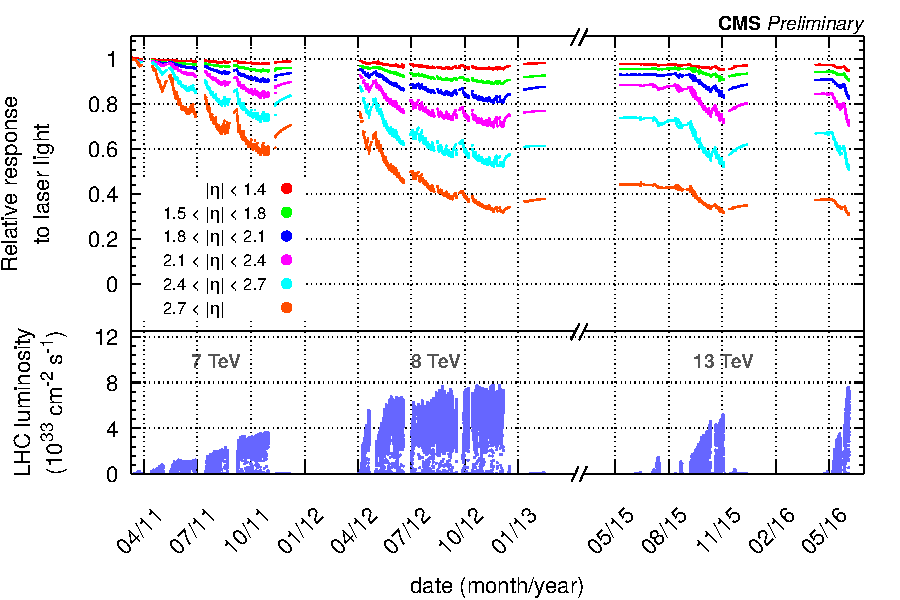
\includegraphics[width=.9\textwidth]{figs/cms/histories_2016.pdf}
\caption{Relative response to laser light from 2011 to 2016, normalized to
  data at the start of 2011~\cite{CMS-DP-2016-031}. An average is shown for each
  pseudorapidity range. The bottom plot shows the corresponding
  instantaneous luminosity. After each LHC technical stop, a
  recovery of crystal transparency is observed.\label{fig:ECALLaserHistory}}
\end{figure}

The ECAL light monitoring system is used to determine corrections,
denoted $S(t)$, to response changes in the ECAL. The
laser light is injected through optical fibers in each crystal. The spectral
composition and the path for the collection of laser light at the
photodetector are different from those for scintillation light. A
conversion factor is required to relate the changes in the ECAL
response to laser light to the changes in the scintillation
signal. The relationship is described by a power law~\cite{CMSECALTDR}:
\begin{equation}
\frac{S(t)}{S_0} = \left(\frac{R(t)}{R_0}\right)^{\alpha}~,
\end{equation}
where $S(t)$ is the channel response to scintillation light at a particular time $t$, $S_0$ is the initial
response, and $R(t)$ and $R_0$ are the corresponding response to laser
light. The exponent $\alpha$ is independent of the loss for small
transparency losses and was measured in test beams to be $1.52$ and
$1.0$ for crystals from the two different
producers, in Russia and China~\cite{VanLysebetten:787485,Adzic:2006za,Ghezzi:934066}.

Alternative forms of these laser corrections, differing in time and
spatial granularity, are utilized at different
stages in the data processing: online at the HLT, during the prompt
reconstruction, and during offline reprocessing of the data. At HLT,
the laser corrections are updated once-per-week and are applied to 11
different $\eta$ rings in each endcap and 17 different $\eta$ rings in
the barrel (the corrections are averaged over each ring). For the prompt reconstruction and the offline
reprocessing of the data, the laser corrections are updated every 40 minutes
and are applied crystal-by-crystal.

The validation of the HLT laser corrections uses a custom workflow which
re-runs the HLT reconstruction on recently collected data with two versions of
laser corrections: the version currently online (and now out-of-date)
and the version to be validated (and up-to-date). An example of a
successfully validated HLT laser correction for a particular week of
data-taking in 2015 is shown in Fig.~\ref{fig:ECALHLT}~\cite{ECALAlCaTwiki}. Unlike the
outdated laser corrections (shown in blue), the updated
laser corrections (shown in black) correct the energy response and
improve the energy resolution for both the endcaps and the barrel.

\begin{figure}\centering
\includegraphics[width=.9\textwidth]{figs/cms/Week42_transpCorr_EB_overlay_IntermediateBlack_oldBlue.png}\\
\includegraphics[width=.9\textwidth]{figs/cms/Week41_transpCorr_EE_overlay_newBlack_oldBlue.png}
\caption{The top (bottom) plot shows the difference between the supercluster energy
  reconstructed at HLT and a reference energy for the ECAL barrel (endcaps) for a particular
  week of data-taking in 2015. The blue data points show the
  difference using the week-old laser corrections, while the solid black histogram shows the reconstructed energy with the
  updated laser correction undergoing validation.\label{fig:ECALHLT}}
\end{figure}
%https://twiki.cern.ch/twiki/bin/viewauth/CMS/EGammaHLT2015LaserCorrValWeeklyReport

The $\Pgh$ and $\pi^0$ meson data are used to validate the laser
corrections for prompt reconstruction and to intercalibrate the energy of ECAL
crystals. The events are selected online by a dedicated calibration trigger with a rate of  8 (2.5) \unit{kHz} in the barrel (endcap), and recorded with
reduced event content, including energy deposits in the ECAL crystals
surrounding a possible $\pi^0$ candidate. A fit is carried out on the invariant mass distribution of the photon
pairs in the mass range of the $\Pgh$ or $\pi^0$ meson. The fit comprises a
polynomial function to describe the background and a Gaussian
distribution to describe the resonance peak. Fig.~\ref{fig:etaEB}
shows an example of the $\pi^0$-meson peak with the fit superimposed,
and the relative value of the fitted $\pi^0$ mass versus time in the barrel for
a period of 8 hours~\cite{CMS-DP-2016-031}. The right plot shows the
energy scale as a function of time, with (green points) and without
(red points) the light monitoring corrections applied, over a period
of 8 hours for data recorded on May 28, 2016 during LHC fill
4958. Each point is obtained from a fit to approximately 8 minutes of data taking. A number of
measurements are possible for each LHC fill, owing to the high
rate for recording $\pi^0$ and $\Pgh$ events. This permits short-term changes in
the ECAL response to be verified before the prompt reconstruction
takes place.


\begin{figure}[bht]
\begin{center}
 %\includegraphics[width=0.40\linewidth,height=5.6cm]{figs/cms/eta_peak.pdf}
 %\includegraphics[width=0.59\linewidth,height=5.6cm]{figs/cms/eta_zoom.pdf}
\includegraphics[height=5.6cm]{figs/cms/Fit_EB_cry.pdf}
\includegraphics[height=5.6cm]{figs/cms/pi0_EB_plus_1.pdf}
%\includegraphics[width=0.49\linewidth]{figs/cms/Fit_EE_cry.pdf}
\end{center}
\caption{\label{fig:etaEB}
 (Left) Invariant mass of photon
pairs reconstructed in one crystal of the ECAL barrel, in
the mass range of the $\pi^0$ meson, during the run 273730 taken in May 2016,
corresponding to an integrated luminosity of approximately 100
pb$^{-1}$. (Right) The stability of the relative energy scale measured from the invariant mass distribution of
$\pi^0$ decays in the ECAL barrel for a typical LHC fill in 2016. The energy scale is measured by fitting
the invariant mass distribution of approximately 200,000 photon pairs
in the mass range of the $\pi^0$ meson. Each point is obtained from a fit
to approximately 8 minutes of data taking. The error bars represent
the statistical errors on the fitted peak position. The energy scale
is plotted as a function of time, over a period of 8 hours for data recorded on May 28, 2016 during LHC fill 4958. The
plot shows the data with (green points) and without (red points) light
monitoring corrections applied. The right-hand panel shows the
projected relative energy scales~\cite{CMS-DP-2016-031}.
%Left: An example of the $\Pgh$-meson peak reconstructed from the invariant
%mass of photon pairs in the barrel, with the result of the fit with a Gaussian
%distribution (continuous line) and a polynomial function (dotted line);
%Right: Stability of the $\Pgh\to\Pgg\Pgg$ mass measurement in the barrel as a
%function of time, over a period of 60 hours, for data recorded in
%September 2011. The plot shows the data with (green points) and
%without (red points) laser corrections applied.
}
\end{figure}

Finally, isolated electrons from $\PW\to\Pe\PGne$ and $Z\to\Pep\Pem$ decays are used to provide an energy
scale to validate the laser corrections over periods of days to
weeks. The event selection is described
in Ref.~\cite{EGM-10-004,Khachatryan:2010xn,CMSPhoton,CMS-DP-2015-065}.
The ratio of the electron energy, $E$, measured in the ECAL, to the
electron momentum, $p$, measured in the tracker, is computed in each
event, and a reference $E/p$ distribution is obtained from the entire
data set after applying laser corrections. The width of the $E/p$
reference distribution is dominated by the energy and momentum
resolution and is not biased by residual imperfections in the laser
corrections. This reference distribution is then scaled to fit
$E/p$ distributions obtained by dividing the same data in groups of
12,000 (5,000) consecutive events for 8\TeV (13\TeV) data recorded in 2012 (2015). The scale factors provide a measure of the
relative response and are shown in Fig.~\ref{fig:wenuEB} for 2012 and
2015 data, as a function of time~\cite{CMSPhoton,CMS-DP-2015-065}. The data are shown before (red open circles) and after
(green filled circles) the laser monitoring corrections are applied. %The magnitude of the average correction for each point is
%indicated by the continuous blue line. 
A stable response to
electromagnetic showers is achieved throughout 2012 (2015) with an RMS of
%0.12\% in the barrel and 0.35\% in the endcaps. This method does not
%require a
0.09\% (0.15\%) in the barrel.
%and 0.28\% in the endcaps. 
This method does not require a knowledge of the absolute calibration of both the energy and the
momentum.

\begin{figure}
\begin{center}
%\begin{tabular}{cc}
% \hspace{-0.5cm}
% \includegraphics[width=0.40\linewidth]{figs/cms/EoP_TypicalFit_EB.pdf} &
% \hspace{-1cm}
% \includegraphics[width=0.69\linewidth]{figs/cms/EsuPhistoryEB.pdf} \\
% \hspace{-0.5cm}
% \includegraphics[width=0.40\linewidth]{figs/cms/EoP_TypicalFit_EE.pdf} &
% \hspace{-1cm}
% \includegraphics[width=0.69\linewidth]{figs/cms/EsuPhistoryEE_alpha116.pdf}
%\end{tabular}
    \includegraphics[width=0.8\linewidth]{figs/cms/stabilityEB.pdf}
    %\includegraphics[width=0.8\linewidth]{figs/cms/stabilityEE.pdf}
    \includegraphics[width=0.8\linewidth]{figs/cms/EB___history_vsTime.pdf}
\end{center}
\caption{\label{fig:wenuEB}
%Relative energy response variation for the barrel (top) and the endcaps (bottom)
%determined from the $E/p$ analysis of electrons in $\PW$-boson decays.
%Left: examples of fits to the $E/p$ distributions before (red) and
%after (green) laser corrections. Middle: Response stability during the
%2011 $\Pp\Pp$ data-taking period before (red open circles) and after
%(green points) response corrections; the blue line shows the inverse
%of the average laser corrections. Right: Distribution of the projected
%relative energy scales.
Ratio of the energy measured by the ECAL over the momentum measured by
the tracker, $E/p$, for electrons selected from $\PW\to\Pe\PGne$ and $Z\to\Pep\Pem$ decays, as a
function of the date at which they were recorded~\cite{CMSPhoton,CMS-DP-2015-065}. The ratio is shown
both before (red open circles) and after (green filled circles) the application of
transparency corrections obtained from the laser monitoring system,
and for the ECAL barrel in 2012 at 8 \TeV (upper plot) and in 2015 at 13\TeV (lower plot). 
Histograms of the values of the measured points, together with
their mean and RMS values are shown beside the main plots.}
\end{figure}

\section{Data scouting}
\label{sec:scouting}

An extension of the alignment/calibration data-taking strategy, referred to as \emph{data
  scouting}, is based on reducing the event size from the default of
$\sim 1$\unit{Megabyte} (MB) in order to increase the recorded event rate and
thus increase physics signal acceptance. This
approach, first implemented at the LHC by the CMS experiment in
2011~\cite{CMS-DP-2012-022}, allows us to increase the physics signal
acceptance of CMS even in the presence of backgrounds with large cross
sections. This is particularly useful in the search for
narrow resonances in the dijet mass spectrum, as described in Ch.~\ref{ch:dijet}, where this strategy allows the search to
be extended into a low-dijet-mass region previously only accessible at
lower-energy colliders~\cite{Khachatryan:2016ecr,CMS-PAS-EXO-16-032}.

Fig~\ref{fig:DataScouting} schematically displays the $H_{\mathrm{T}}$
thresholds used for the different varieties of data scouting during the
2015 and 2016 runs and Fig~\ref{fig:DataScoutingContent} displays the
corresponding event content~\cite{AndersonScouting}. \emph{Calo scouting}, which selects
events based only on Calo jets and records only calorimetric
information, has a very small event size of $\sim 1.5$\unit{kilobyte} (kB), allowing the
rate to go as a high as 3.8 \unit{kHz}. Meanwhile, \emph{PF scouting},
which runs the full PF algorithm and records all PF-reconstructed
information, including leptons, photons, and jets with \cPqb-tagging
information, has a larger event size $\sim 10$\unit{kB}. In order to stay within the
HLT timing budget, the maximum permissible rate is 720\unit{Hz}. Simultaneously, the \emph{data parking} stream sends the
full raw events from PF scouting directly to tape without reconstruction. This
multifaceted approach is advantageous in the case that a signal is
seen in the scouting data that warrants more investigation.

\begin{figure}\centering
\includegraphics[width=.9\textwidth]{figs/cms/Scouting2015.pdf}\\
\includegraphics[width=.9\textwidth]{figs/cms/Scouting2016.pdf}
\caption{HLT $H_\mathrm{T}$ thresholds for Calo and PF scouting for
  2015 (top) and 2016 (bottom) data-taking runs~\cite{AndersonScouting}. The
  rates for the 2015 (2016) are normalized to an instantaneous luminosity
  of $7\times 10^{33}$ cm$^{-2}$ s$^{-1}$ ($10^{34}$ cm$^{-2}$
  s$^{-1}$). \label{fig:DataScouting}}
\end{figure}

\begin{figure}\centering
\includegraphics[width=.45\textwidth]{figs/cms/pfscoutingeventcontent.png}
\includegraphics[width=.45\textwidth]{figs/cms/caloscoutingeventcontent.png}
\caption{The event content for PF scouting (left) consists of PF
  candidates, anti-$\kt$ $R=0.4$ PF jets, PF $\MET$, reconstructed vertices,
  PF-reconstructed electrons, muons, photons, and the median energy density in an event $\rho$, which amounts to
  $\sim 10$\unit{kB}. The event content for Calo scouting (right),
  consists of anti-$\kt$ $R=0.4$ Calo jets, Calo $\MET$, vertices (if
  another trigger reconstructed them for this event), and the median energy
  density in an event $\rho$, which amounts to $\sim 1.5$\unit{kB}~\cite{AndersonScouting}.\label{fig:DataScoutingContent}}
\end{figure}

\chapter{Topological HLT development at $\sqrt{s}=13 \TeV$}
\label{ch:hlt13TeV}

Traditionally, trigger algorithms employed at hadron colliders consisted
of selecting events based on the presence of specific particles, such
as leptons or photons, above some energy threshold and isolated from
the rest of the event. In other trigger algorithms, global
event properties (such as ``sum'' quantities like the hadronic transverse energy $H_{\mathrm{T}}$
or the missing transverse energy $\MET$) were also used. 

The event selection used in modern searches for beyond-the-standard-model
(BSM) physics employ new techniques, such as kinematic variables like
\MR and \Rtwo, that no longer map on to these traditional trigger
requirements. Fortunately, the flexibility of
the software-based system allowed the development of dedicated trigger paths, based
on sophisticated kinematic variables and specific event topologies.

To target a broad range of new physics possibilities, we designed four different
types of triggers for use in $\sqrt{s}=13\TeV$ $\Pp\Pp$ collisions:
\begin{itemize}
\item Dijet razor trigger with hyperbolic \MR and \Rtwo requirements
  targeting the squark pair production topology;
\item Quadjet razor trigger with hyperbolic \MR and \Rtwo requirements
  targeting top-squark or gluino pair production topologies;
\item High-\Rtwo trigger targeting dijet+invisible topologies with
  large transverse momentum imbalance; and
\item Razor $\PH(\bbbar)$ trigger targeting production of Higgs boson
  decaying to a bottom quark-antiquark pair ($\PH\to\bbbar$) in
  association with a jet and possibly some missing transverse energy,
  i.e. $\PH(\bbbar)+\mathrm{jet}+\mathrm{invisible}$.
\end{itemize}

The dijet and quadjet razor triggers are broadly motivated by SUSY pair
production and represent an update and incremental improvement of the razor triggers
used in previous searches at $\sqrt{s}=8\TeV$~\cite{razor8TeV}. Both
sets of triggers are based on hyperbolic thresholds in the $(\MR,\Rtwo)$
plane, with the 2015 updated thresholds shown in
Fig~\ref{fig:hyperbolic}. The 2015 hyperbolic contours follow the
iso-probability contours $(\Rtwo+0.25)(\MR+300\GeV)=\mathrm{constant}$, derived from the background-only fit to the MultiJet category
in the 8\TeV razor search performed using 2012 data. This implies that
these hyperbolic contours efficiently reject background, while
maintaining a large acceptance for SUSY signal models with a large
characteristic mass scale $M_{\Delta}\gtrsim 500 \GeV$ and sufficient
transverse momentum imbalance. Another update is that the 13 \TeV razor triggers are based on PF-reconstructed objects rather
than Calo jets and muons, which means that the online $\Rtwo$ variable is
much more correlated with the offline $\Rtwo$ variable, which is also
PF-based. This leads to an improved trigger efficiency plateau of
$97\%$ for 2015 (compared to $95\%$ in 2012), shown in Fig.~\ref{fig:turnons}.

\begin{figure}[htb!]
\centering
\includegraphics[width=0.8\textwidth]{figs/hlt13TeV/HLTRsqMR.pdf}
\caption{\label{fig:hyperbolic} Hyperbolic and baseline thresholds in
  \Rtwo and \MR used in the dijet and quadjet razor triggers. The
  hyperbolic thresholds are of the form $(\Rtwo+0.25)(\MR+300\GeV)=\mathrm{constant}$.}
\end{figure}

\begin{figure}[ht!]
\centering
\includegraphics[width=0.7\textwidth]{figs/hlt13TeV/turnons_2015_no100GeVmuons_thesis/HLT_RsqMR240_Rsq0p09_MR200_HLT_RsqMR240_Rsq0p09_MR200_4jet_HLT_Rsq0p25_HLT_Ele27_eta2p1_WPLoose_Gsf_effRsq_MR500.pdf}
\includegraphics[width=0.7\textwidth]{figs/hlt13TeV/turnons_2015_no100GeVmuons_thesis/HLT_RsqMR240_Rsq0p09_MR200_HLT_RsqMR240_Rsq0p09_MR200_4jet_HLT_Rsq0p25_HLT_Ele27_eta2p1_WPLoose_Gsf_effMR_Rsq0p25.pdf}
\includegraphics[width=0.7\textwidth]{figs/hlt13TeV/turnons_2015_no100GeVmuons_thesis/HLT_RsqMR240_Rsq0p09_MR200_HLT_RsqMR240_Rsq0p09_MR200_4jet_HLT_Rsq0p25_HLT_Ele27_eta2p1_WPLoose_Gsf_eff2D.pdf}
\caption{\label{fig:turnons} Trigger efficiency of the boolean ``or'' of
  the dijet, quadjet and high-\Rtwo triggers as used in the search of
  Ch.~\ref{ch:analysis13TeV}, measured in a data sample of
  single-electron events as a function of $\Rtwo$ (top), $\MR$ (middle), and as a function of $(\MR,\Rtwo)$ (bottom).}
\end{figure}

The high-\Rtwo trigger is motivated by the search for the direct
production of dark matter (DM) particles at the
LHC~\cite{Khachatryan:2016reg}.  DM particles themselves
would not leave a detectable signal in the detector, but if
they were produced in association with high-energy quarks or gluons,
they could produce signatures with jets and transverse
momentum imbalance. The traditional approach, employed by both CMS and
ATLAS, is to search in events with one high-$\pt$ jet and large $\MET$
(so-called monojet searches)~\cite{Aad:2011xw,Chatrchyan:2012me}. A complementary
approach is to search in events with at least two jets passing a looser
event selection using the razor variables. The sensitivity of these variables to direct DM production was
suggested in Ref.~\cite{Fox:2012ee}, and the search carried out by CMS
demonstrates that the resulting sensitivity is comparable to that of
monojet searches~\cite{Fox:2012ee,Papucci:2014iwa,Khachatryan:2016reg}.
The hallmark of many direct DM production models in the razor plane is
a peaking behavior near $\Rtwo\gtrsim 0.8$ and an exponentially
falling $\MR$ distribution with no special structure. For this reason,
the high-\Rtwo trigger is designed with a threshold in \Rtwo but no
requirement on \MR to allow for greater DM signal acceptance.

Finally, the razor $\PH(\bbbar)$ trigger is motivated by an
excess observed in Run 1 by CMS in events with a Higgs boson decaying
to two photons ($\PH\to\Pgg\Pgg$) plus at least one extra jet~\cite{RazorHgaga}. The excess,
corresponding to a local significance of
$2.9\sigma$, consists of five events observed with $400\GeV<\MR<1400
\GeV$,  $\Rtwo>0.05$, and $m_{\Pgg\Pgg}$ consistent with $m_\PH= 125
\GeV$ in a high-resolution diphoton category, compared to less than one
expected background event. The general idea is to search for a similar
signature in the $\PH\to\bbbar$ channel, which comes with a larger
signal yield (90,000 times more assuming SM Higgs branching ratios),
but a much larger background, resulting in a considerably worse
signal-to-background ratio and a much larger background event rate. These final
two features make the definition of an optimal trigger strategy much more
challenging than in the $\PH\to\Pgg\Pgg$ decay channel. Given this, the trigger
requirements of three jets, two \cPqb-jets, $\MR>300
\GeV$, $\Rtwo>0.02$, and $m_{\bbbar}$ roughly consistent with $m_\PH= 125
\GeV$ are chosen to (a) maintain signal acceptance based on the observed
features, (b) accept additional events outside of the $m_\PH$ window
to permit a robust background estimation based on a fit, and (c)
limit the rate and average CPU time of the trigger to an acceptable
level.

For each trigger, we developed two different versions: a ``main''
version intended for $7\times 10^{33}$ cm$^{-2}$ s$^{-1}$ and 20 average
pileup interactions, and a ``backup'' version, with tighter thresholds
intended for $1.4\times 10^{34}$ cm$^{-2}$ s$^{-1}$ and 40 average
pileup interactions. The correspondence between the purpose of each
trigger and its path name is shown in Tab.~\ref{tab:pathnames}. Each trigger path name encodes the main
  selection criteria. For the dijet and quadjet triggers, ``RsqMR240'' denotes the hyperbolic
  threshold $(\Rtwo+0.25)(\MR+300\GeV)=240\GeV$, ``Rsq0p09\_MR200''
  denotes the baseline thresholds $\Rtwo>0.09$ and $\MR>200\GeV$, and ``4jet'' denotes a
  four-jet requirement where the two leading (remaining) jets are required to have
  a minimum $\pt$ of $50\GeV$ ($40\GeV$). For the $\PH(\bbbar)$
  trigger, ``TriPFJet80\_60\_40'' denotes a three-jet requirement where the
  leading, subleading, and remaining jet is required have a
  minimium \pt of $80\GeV$, $60\GeV$, and $40\GeV$, respectively, 
``DoublePFBTagCSV0p7\_0p4'' denotes a two \Pqb-tagged jet
  requirement, with CSV discriminator values above 0.7 and 0.4,
  respectively, and ``Mbb60\_200'' denotes the
  $60<m_{\bbbar}<200\GeV$ mass window.

\begin{table*}[ht!]
\centering
 \caption{Correspondence between the purpose of each
trigger and its path name.\label{tab:pathnames}}
\resizebox{\textwidth}{!}{
\begin{tabular}{l|l}
\hline\hline
Trigger path  & Purpose \\
\hline
HLT\_RsqMR240\_Rsq0p09\_MR200 & main dijet trigger\\
HLT\_RsqMR270\_Rsq0p09\_MR200 & backup dijet trigger \\
HLT\_RsqMR240\_Rsq0p09\_MR200\_4jet & main quadjet trigger \\
HLT\_RsqMR270\_Rsq0p09\_MR200\_4jet & backup quadjet trigger \\
HLT\_Rsq0p25 & main high-\Rtwo trigger \\
HLT\_Rsq0p30 & backup high-\Rtwo trigger \\ 
HLT\_Rsq0p02\_MR300\_TriPFJet80\_60\_40\_&\multirow{2}{*}{main $\PH(\bbbar)$ trigger} \\
~DoublePFBTagCSV0p7\_0p4\_Mbb60\_200 & \\
HLT\_Rsq0p02\_MR300\_TriPFJet80\_60\_40\_ & \multirow{2}{*}{backup $\PH(\bbbar)$ trigger}  \\
~DoublePFBTagCSV0p7\_Mbb60\_200 & \\
\hline\hline
\end{tabular}}
\end{table*}

\section{HLT path design}

The design of the four main HLT paths in terms of producers (in
purple) and filters (in blue) is shown
in Fig.~\ref{fig:HLTdesign}. The first step is always a filter, which
rejects events with no hadronic activity above a certain threshold reconstructed by the L1 trigger.
As detailed in Sec.~\ref{sec:trigger}, there are two main technical
constraints an HLT path must satisfy: (a) the average CPU time required must be
small enough so that the entire HLT menu fits within the timing budget
 of $\sim160$ \unit{ms} per event and (b) the rate must
be small enough so that the entire HLT menu fits within the maximum
allowable rate  of $\sim1$ \unit{kHz}. To satisfy the timing
requirement, all the paths are outfitted with
calorimetric prefilters. The aim of these prefilters is to reject
events based only on information from the calorimeters, whose
reconstruction algorithms are much faster than the PF algorithm. In
other words, to keep the timing of the paths manageable, it is
necessary to limit the input rate to the PF algorithm. Thus, all four
triggers have a prefilter based on calorimeter-based versions of the razor
variables.

\begin{figure}[ht!]
\centering
\includegraphics[width=0.8\textwidth,clip=true,viewport=0 110 1024
500]{figs/hlt13TeV/HLTDijetDesign.pdf}\\
(a) HLT\_RsqMR240\_Rsq0p09\_MR200 \\
\includegraphics[width=0.8\textwidth,clip=true,viewport=0 110 1024
500]{figs/hlt13TeV/HLTQuadjetDesign.pdf}\\
(b) HLT\_RsqMR240\_Rsq0p09\_MR200\_4jet \\
\includegraphics[width=0.8\textwidth,clip=true,viewport=0 220 1024
500]{figs/hlt13TeV/HLTR2Design.pdf}\\
(c) HLT\_Rsq0p25\\
\includegraphics[width=0.8\textwidth,clip=true,viewport=0 110 1024
500]{figs/hlt13TeV/HLTRazorHbbDesign.pdf}\\
(d) HLT\_Rsq0p02\_MR300\_TriPFJet80\_60\_40\_\\
~DoublePFBTagCSV0p7\_0p4\_Mbb60\_200
\caption{\label{fig:HLTdesign} Flow of the producer steps (in purple)
  and filter steps (in blue) in
  the razor triggers.}
\end{figure}

\section{HLT rate and average CPU time}

The HLT rates and average CPU time consumed per event for the both the main and
backup razor triggers, as measured in data collected in 2015, are
presented in Tab.~\ref{tab:rates2015}. The thresholds on the razor
variables, jet $\pt$, and \cPqb-tag discriminator values, and were all
optimized to achieve an acceptable level of added rate and added CPU
time per event with respect to the rest of HLT menu (taking into
account overlapping events and reused algorithms) for the full suite of razor triggers. 

%\begin{table*}[ht!]
%\centering
% \caption{Rates for 0\unit{T} triggers.
% \label{tab:rates0T}}
%\resizebox{\textwidth}{!}{
%\begin{tabular}{l|l|l}
%\multirow{2}{*}{Trigger path} &  Data rate (run 260039) & MC rate (Spring '15) \\
% &  $4\times 10^{33}$ \unit{cm$^{-2}$ s$^{-1}$}, 17 PU &  \\\hline
%HLT\_Rsq0p25\_Calo & 3.7 Hz & \\
%HLT\_RsqMR240\_Rsq0p09\_MR200\_4jet\_Calo & 5.6 Hz & \\
%HLT\_RsqMR240\_Rsq0p09\_MR200\_Calo & 18.2 Hz & 
%\end{tabular}}
%\end{table*}

\begin{table*}[ht!]
\centering
 \caption{HLT rates and average CPU time consumed for the main and
   backup razor triggers under different running conditions in 2015. Run 260627 had $5\times 10^{33}$ cm$^{-2}$
   s$^{-1}$ peak instantaneous luminosity with 17 average pileup
   interactions, while run 259721 had $1.5\times 10^{33}$ cm$^{-2}$
   s$^{-1}$ peak instantaneous luminosity with 23 average pileup interactions. \label{tab:rates2015}}
\resizebox{\textwidth}{!}{
\begin{tabular}{l|c|c}
\hline\hline
\multirow{4}{*}{Trigger path} &  Data rate [Hz] & CPU time [ms]\\
& Run 260627 & Run 259721\\
 &  $5\times 10^{33}$ cm$^{-2}$ s$^{-1}$ &  $1.5\times 10^{33}$
                                          cm$^{-2}$ s$^{-1}$ \\
& 17 PU  & 23 PU\\
\hline
HLT\_RsqMR240\_Rsq0p09\_MR200 & 7.7 & 27 \\ 
HLT\_RsqMR270\_Rsq0p09\_MR200 & 2.3 & 17  \\ 
HLT\_RsqMR240\_Rsq0p09\_MR200\_4jet & 1.2 & 20 \\
HLT\_RsqMR270\_Rsq0p09\_MR200\_4jet & 0.5 & 15 \\
HLT\_Rsq0p25 & 0.7 & 14 \\
HLT\_Rsq0p30 & 0.4 & 14  \\
HLT\_Rsq0p02\_MR300\_TriPFJet80\_60\_40\_&\multirow{2}{*}{16.0} & \multirow{2}{*}{34}\\
~DoublePFBTagCSV0p7\_0p4\_Mbb60\_200 & &\\
HLT\_Rsq0p02\_MR300\_TriPFJet80\_60\_40\_ & \multirow{2}{*}{8.0} & \multirow{2}{*}{26}\\
~DoublePFBTagCSV0p7\_Mbb60\_200 & & \\
\hline\hline
\end{tabular}}
\end{table*}
% timing from: 
% https://docs.google.com/spreadsheets/d/1qu0dKZfjHEl073QyXayxzPBNoT10GZKMiPU9-z8VSeU/edit#gid=0
% supplemented by my measurement (for RsqMR240...)
% https://www.dropbox.com/s/z8qfx57du7h3gzq/TSG_RazorHLT2016_30Mar2016.pdf?dl=0


\section{Pileup dependence of HLT rate}
\label{sec:pileuphlt}
The HLT rate, normalized by the number of colliding bunches, as a function of the number of pileup interactions for
each razor trigger and for different data runs collected in 2015 is
shown in Figures~\ref{fig:HLTpileup1}~and~\ref{fig:HLTpileup2}. Nominally, the dependence of the
normalized HLT rate on pileup is expected to be linear, as is the case
for single-object triggers. In contrast, triggers based on sum quantities
(such as $H_\mathrm{T}$ or $\MET$) and multi-object triggers often
demonstrate a nonlinear dependence on pileup, not due to a physical
increase in the cross section of the selected physics processes, but rather due to the effects of pileup
contamination~\cite{Bocci:2016}. To illustrate this, consider the
case of a QCD dijet event with no true $\MET$. Normally such an event
would be rejected by $\MET$ triggers that require $\MET$ above some
threshold, but if some jets from pileup interactions are misinterpreted as part of the
event-of-interest then the HLT-reconstructed $\ptvecmiss$ will be
$-\sum_{j\in\mathrm{pileup}} \vecpt^{\,j}$, which may not perfectly balance to
zero as illustrated in Fig.~\ref{fig:pileupjet}.

\begin{figure}[ht!]
\centering 
\includegraphics[width=0.7\textwidth]{figs/hlt13TeV/pileupjet.pdf}
\caption{\label{fig:pileupjet} Pileup jet misinterpreted as part of
  the main interaction event.}
\end{figure}

As the razor triggers are both based on sum quantities and multiple objects,
they also exhibit some nonlinear dependence on pileup. This implies
that as the pileup increases at the LHC in 2016 and beyond, either trigger thresholds
will need to rise dramatically or more sophisticated methods to deal
with pileup contamination will need to implemented. One such method is
delineated in Ch.~\ref{ch:timing}.

\begin{figure}[ht!]
\centering 
\includegraphics[width=0.9\textwidth]{figs/hlt13TeV/linear/HLT_RsqMR240_Rsq0p09_MR200_instLumi_vs_rawRate.pdf}\\
(a) HLT\_RsqMR240\_Rsq0p09\_MR200 \\
\includegraphics[width=0.9\textwidth]{figs/hlt13TeV/linear/HLT_RsqMR240_Rsq0p09_MR200_4jet_instLumi_vs_rawRate.pdf}\\
(b) HLT\_RsqMR240\_Rsq0p09\_MR200\_4jet
\caption{\label{fig:HLTpileup1} Pileup dependence of the dijet (a) and
  quadjet (b) razor triggers throughout 2015. Each data point
  corresponds to a different luminosity section (23.3 seconds of data-taking). The legend denotes the
  run number and number of colliding bunches in each run.}
\end{figure}

\begin{figure}[ht!]
\centering 
\includegraphics[width=0.9\textwidth]{figs/hlt13TeV/linear/HLT_Rsq0p25_instLumi_vs_rawRate.pdf}\\
(c) HLT\_Rsq0p25\\
 \includegraphics[width=0.9\textwidth]{figs/hlt13TeV/linear/HLT_Rsq0p02_MR300_TriPFJet80_60_40_DoublePFBTagCSV0p7_0p4_Mbb60_200_instLumi_vs_rawRate.pdf}\\
(d) HLT\_Rsq0p02\_MR300\_TriPFJet80\_60\_40\_\\
~DoublePFBTagCSV0p7\_0p4\_Mbb60\_200
\caption{\label{fig:HLTpileup2} Pileup dependence of the high-\Rtwo
  (c) and $\PH(\bbbar)$ (d) razor triggers. Each data point
  corresponds to a different luminosity section (23.3 seconds of data-taking). The legend denotes the
  run number and number of colliding bunches in each run.}
\end{figure}



\chapter{Searches for Supersymmetry at $\sqrt{s}=8\TeV$}
\label{ch:analysis8TeV}

\section{Event selection}
\label{sec:selection}
Events are selected at the L1 trigger level by requiring at least two
jets with $|\eta|<3$. At the HLT level, events are selected using
dedicated razor algorithms, consisting of a loose selection on \MR and
$\Rtwo$. Razor-specific triggers are used in the HLT in order to avoid
biases on the shapes of distributions from the SM background that are
introduced by requirements on more traditional selection variables
such as $\ETm$.  The razor triggers reject the majority of the SM
background, which mostly appears at low $\Rtwo$ and low $\MR$, while
retaining events in the signal-sensitive regions of the ($\MR$,
$\Rtwo$) plane. Two types of triggers are used: i) a hadronic razor
trigger, which selects events that contain at least two jets with
transverse momentum $\pt>64\GeV$ by applying threshold requirements on
$\Rtwo$, $\MR$, and their product; ii) a muon and electron razor
trigger, which selects events with at least one isolated electron or
muon with $\pt>12\GeV$ in combination with looser requirements on
$\Rtwo$, $\MR$, and their product. The trigger efficiency, evaluated
using a dedicated trigger, is measured to be $(95 \pm 5)\%$ and is
independent of $\Rtwo$ and $\MR$ for the events selected with the
baseline requirements described in Chapter~\ref{ch:kinematic}.

Following the trigger selection, events are required to contain at
least one reconstructed interaction vertex. If more than one vertex is
found, the one with the highest $\pt^2$ sum of associated tracks is
chosen as the interaction point for event reconstruction. Algorithms are
used to remove events with detector- and beam-related noise that can
mimic event topologies with high energy and large $\pt$
imbalance~\cite{Chatrchyan:2011tn,Chatrchyan:2012lia,Khachatryan:2014gga}.

The analysis uses a global event description based on the CMS particle
flow (PF) algorithm~\cite{PF1,PF2}. Individual particles (PF
candidates) are reconstructed by combining the information from the inner
tracker, the calorimeters, and the muon system. Five categories of PF
candidates are defined: muons, electrons, photons (including their
conversions to $\Pep\Pem$ pairs), charged hadrons, and neutral
hadrons. The contamination from other proton-proton collisions in the
same or in neighboring bunch crossings is reduced by discarding the
charged PF candidates not compatible with the interaction point. When
computing lepton isolation and jet energy, the corresponding
contamination from neutral particles is subtracted on average by
applying an event-by-event correction based on the jet-area
method~\cite{jetarea_fastjet,jetarea_fastjet_pu,JME-JINST}.

A ``tight'' lepton identification is used for muons and electrons,
consisting of requirements on isolation and track reconstruction
quality. For electrons, the shape and position of the energy deposit
in the electromagnetic calorimeter is used to further reduce the contamination from
hadrons~\cite{Chatrchyan:2013iaa}. For events with one identified
tight lepton, additional muons or electrons are identified through a
``loose'' lepton selection, characterized by a relaxed isolation
requirement~\cite{Chatrchyan:2013mxa}. Tight leptons are
required to have $\pt>15$\GeV and loose leptons $\pt>10$\GeV.

Jets are reconstructed by clustering the PF candidates with the
\textsc{FastJet}~\cite{fastjet} implementation of the anti-\kt~\cite{antikt} algorithm with the distance parameter $R=0.5$. We
select events containing at least two jets with $\pt>80$\GeV and
$\abs{\eta}<2.4$, representing a tighter version of the L1 jet selection criterion. The $\pt$
imbalance in the event, $\ptvecmiss$, is the
negative of the sum of the $\ptvec$ of the PF candidates in the
event. Its magnitude is referred to as $\ETm$. For each event, the $\ptvecmiss$ and the
four-momenta of all the jets with $\pt>40$\GeV and $\abs{\eta}<2.4$ are
used to compute the razor variables, as described in
Section~\ref{sec:razVar}.

The medium working point of the combined secondary vertex
algorithm~\cite{btag8TeV} is used for b-jet tagging. The \PQb-tagging
efficiency and mistag probability are measured from data control
samples as a function of the jet $\pt$ and $\eta$. Correction factors
are derived for Monte Carlo (MC) simulations through comparison of the
measured and simulated \PQb-tagging efficiencies and mistag rates found
in these control samples~\cite{btag8TeV}.

Events with no \PQb-tagged jet are discarded, a criterion motivated by
the natural SUSY signatures described in Section~\ref{sec:sms}. A tighter
requirement ($\geq$2 \PQb-tagged jets) is imposed on events without an
identified tight lepton and fewer than four jets. This requirement reduces the
expected background from SM production of $\cPZ(\to\nu\bar\nu)$+jets
events to a negligible level.


\section{Box definitions}
\label{sec:razVar}

The selected events are categorized into the different razor boxes according to
their event content as shown in Table~\ref{tab:boxDef}. In the table,
the boxes are listed according to the filling order, from the first
(at the top of the table) to the last (at the bottom). If an event
satisfies the requirements of two or more boxes, the event is assigned
to the first listed box to ensure the boxes correspond to disjoint samples.

The events in the single-lepton and two-lepton boxes are recorded
using the electron and muon razor trigger. The remaining two boxes, generically
referred to as ``hadronic'' boxes, contain events recorded using the
hadronic razor trigger.

In the two-lepton boxes, the ($\MR$, $\Rtwo$)
distribution of events with at least one \PQb-tagged jet is studied. For
the other boxes, the data are binned according to the \PQb-tagged jet
multiplicity: 1 \PQb-tag, 2 \PQb-tags, and $\geq$3 \PQb-tags.

\begin{table*}[ht!]
\centering
 \caption{Kinematic and multiplicity requirements defining the nine
 razor boxes. Boxes are listed in order of event filling priority.
 \label{tab:boxDef}}
\resizebox{\textwidth}{!}{
\begin{tabular}{ccccc}
Box & Lepton & \PQb-tag & Kinematic & Jet \\
\hline
 \multicolumn{5}{c}{Two-lepton boxes}\\
\hline
\multirow{2}{*}{MuEle} & $\geq$1 tight electron and & \multirow{6}{*}{$\geq$1 \PQb-tag} & \multirow{2}{*}{} & \multirow{6}{*}{$\geq$2 jets}\\
& $\geq$1 loose muon & & & \\
\cline{1-2}
\multirow{2}{*}{MuMu} & $\geq$1 tight muon and & & ($\MR >300$\GeV and $\Rtwo > 0.15$) and & \\
& $\geq$1 loose muon & & ($\MR > 350$\GeV  or $\Rtwo > 0.2$) & \\
\cline{1-2}
\multirow{2}{*}{EleEle} & $\geq$1 tight electron and & & & \\
& $\geq$1 loose electron& & & \\
\hline
\multicolumn{5}{c}{Single-lepton boxes}\\
\hline
MuMultiJet & 1 tight muon & \multirow{4}{*}{$\geq$1 \PQb-tag} & & \multirow{2}{*}{$\geq$4 jets} \\
%\cline{1-2}
EleMultiJet &1 tight electron & & ($\MR > 300$\GeV and $\Rtwo > 0.15$) and & \\
%\cline{1-2}
\cline{5-5}
MuJet & 1 tight muon & & ($\MR > 350$\GeV or $\Rtwo > 0.2$) & \multirow{2}{*}{2 or 3 jets}\\
%\cline{1-2}
EleJet & 1 tight electron & & &  \\
\hline
\multicolumn{5}{c}{Hadronic boxes}\\
\hline
MultiJet & none & $\geq$1 \PQb-tag & ($\MR > 400$\GeV and $\Rtwo > 0.25$) and &$\geq$4 jets\\
%\cline{1-3}
%\cline{5-5}
$\geq$2 \PQb-tagged jet & none & $\geq$2 \PQb-tag &  ($\MR > 450$\GeV or $\Rtwo > 0.3$) & 2 or 3 jets\\
\end{tabular}}
\end{table*}

A baseline kinematic requirement is applied to define the region in
which we search for a signal:
\begin{itemize}
\item $\MR>400$\GeV and $\Rtwo>0.25$ for the hadronic boxes;
\item $\MR>300$\GeV and $\Rtwo>0.15$ for the other boxes.
\end{itemize}
The tighter baseline selection for the hadronic boxes is a consequence
of the tighter threshold used for the hadronic razor trigger. The
kinematic plane defined by the baseline selection is divided into three
regions (see Fig.~\ref{fig:regions}):
\begin{itemize}
\item Low \MR sideband: $400<\MR<550$\GeV
 and $\Rtwo>0.30$ for the hadronic boxes;
 $300<\MR<450$\GeV and $\Rtwo>0.20$ for the other
 boxes.
\item Low  \Rtwo sideband: $\MR>450$\GeV and
  $0.25<\Rtwo<0.30$ for the hadronic boxes;
  $\MR>350$\GeV and $0.15<\Rtwo<0.20$ for the other
  boxes.
\item Signal-sensitive region: $\MR>550$\GeV and
 $\Rtwo>0.30$ for the hadronic boxes; $\MR>450$\GeV
 and $\Rtwo>0.20$ for the other boxes.
\end{itemize}
The bottom left corner of the razor plane, not included in any of the
three regions, is excluded from the analysis. Given this selection,
the multijet background from quantum chromodynamics processes is
reduced to a negligible level due to the fact that these processes
typically peak at $\Rtwo\approx0$ and fall exponentially for
larger values of $\Rtwo$~\cite{razorPRL,razorPRD}.

\begin{figure}[ht!]
\centering
\includegraphics[width=0.49\textwidth]{figs/analysis8TeV/SidebandL_MultiJet.pdf}
\includegraphics[width=0.49\textwidth]{figs/analysis8TeV/SidebandL_Mu.pdf}
\caption{\label{fig:regions} Definition of the sideband and the
 signal-sensitive regions used in the analysis, for (left) the hadronic
 boxes and (right) the other boxes.}
\end{figure}

\section{Modeling of the standard model backgrounds}
\label{sec:bmodel}
Under the hypothesis of no contribution from new-physics processes,
the event distribution in the considered portion of the
($\MR$, $\Rtwo$) plane can be described by the sum of
the contributions from SM $\cPV$+jets events (where
$\cPV$ indicates a $\PW$ or $\cPZ$ boson) and SM top quark-antiquark and
single-top events, where the events with a top quark are generically
referred to as the $\ttbar$ contribution. Based on MC studies, the
contributions from other processes are determined to be
negligible.

We study each of these processes using MC samples, generated with the
\MADGRAPH v5
simulation~\cite{Alwall:2011uj,Alwall:2014hca}. Parton shower and
hadronization effects are included by matching events to the \PYTHIA v6.4.26 simulation~\cite{Sjostrand:2006za} using the MLM
algorithm~\cite{Hoche:2006ph}. The events are processed by a
\GEANT-based~\cite{G4} description of the CMS apparatus in order to
account for the response of the detector.

Once normalized to the NLO inclusive cross
section and the integrated luminosity, the absolute yield of the
$\cPV$+jets events contribution satisfying the event selection is found
to be negligible in all of the two-lepton boxes. In the remaining boxes,
its contribution to the total SM background is found to be
approximately 25\%. The contribution of $\cPV$+jets events in
the $\geq$2 \PQb-tag and the $\geq$4 jet sample is found to be
negligible. The remainder of the background in each box originates
from $\ttbar$ events.

\subsection{Empirical Razor Function}
Based on the study of the data collected at $\sqrt{s}=7\TeV$ and the
corresponding MC samples~\cite{razorPRL,razorPRD}, the two-dimensional
probability density function
$P_\mathrm{SM}(\MR,\Rtwo)$ for each SM process is
found to be well described by the empirical function
\begin{equation}
 f(\MR,\Rtwo) =  \bigl[b(\MR-{\MRz})^{1/n}(\Rtwo-{\Rtwoz})
  ^{1/n}-1\bigr]\re^{-bn(\MR-{\MRz})^{1/n}(\Rtwo-{\Rtwoz})
    ^{1/n}} ,
\label{eq:razFun}
\end{equation}
where $b$, $n$, $\MRz$, and $\Rtwoz$ are free
parameters of the background model. 

For $n=1$, this function recovers the two-dimensional exponential function used for previous
studies~\cite{razorPRL,razorPRD}. The original motivation is detailed
in the cited papers, but a quick summary follows. There is an observed
correlation between the two razor variables such that after a baseline
selection $\MR>\MR^{\mathrm{min}}$ and $\Rtwo>\Rtwo_{\mathrm{min}}$, the distributions of the SM backgrounds
exhibit an exponential behavior in $\Rtwo$ ($\MR$) when integrated over
$(\MR)$, ($\Rtwo$):
\begin{align}
 \int^{\infty}_{\Rtwo_{\mathrm{min}}} P_\mathrm{SM}(\MR,\Rtwo)
  \mathrm{d}\Rtwo &\propto e^{-(r_0 + r_1\Rtwo_{\mathrm{min}})M_R}~,\\
 \int^{\infty}_{\MR^{\mathrm{min}}} P_\mathrm{SM}(\MR,\Rtwo)
  \mathrm{d}\MR &\propto  e^{-(m_0+ m_1\MR^{\mathrm{min}})\Rtwo}~,
\label{eq:2dcorrelation}
\end{align}
where $r_0$, $r_1$, $m_0$, and $m_1$ are interrelated exponential parameters.
This behavior for QCD multijets background is illustrated in
Fig.~\ref{fig:qcdfit}. The empricial function in Eqn.~\ref{eq:razFun} with
$n=1$ perfectly replicates this behavior and the exponential parameters can be identified with
the empirical function's parameters, namely $r_0 = - b\Rtwoz$, $m_0 = - b\MRz$, and $r_1=m_1=b$.

\begin{figure}[tb!]
\centering
\includegraphics[width=0.49\textwidth]{figs/analysis8TeV/qcd-mr-prd.pdf}
\includegraphics[width=0.49\textwidth]{figs/analysis8TeV/qcd-rsq-prd.pdf}\\
\includegraphics[width=0.49\textwidth]{figs/analysis8TeV/qcd-slopeMR-prd.pdf}
\includegraphics[width=0.49\textwidth]{figs/analysis8TeV/qcd-slopeR-prd.pdf}
\caption{QCD multijet events collected by CMS at $\sqrt{s}=7\TeV$
  demonstrate the two-dimensional correlation between $\MR$ and
  $\Rtwo$ that motivates the original functional form.\label{fig:qcdfit}}
\end{figure}

To account for the possibility of non-exponential tails of the SM
backgrounds, the $\sqrt{s}=7\TeV$ search invoked two copies of the
empirical function with $n=1$ to model each SM background. 
For the $\sqrt{s}=8\TeV$ search, we take a different approach by using
only one instance of the function, but allowing the $n$ parameter to deviate
from $1$. Fig.~\ref{fig:twoexp} illustrates the similarity between using two exponential components and using one
instance of the generalized function.

\begin{figure}[tb!]
\centering
\includegraphics[width=0.8\textwidth,clip=true,viewport= 0 70 600 410]{figs/analysis8TeV/twoexp.pdf}
\caption{Two exponential components with $n=1$ and their sum are shown in blue compared with
  a single modified exponential with $n=3$ in black.\label{fig:twoexp}}
\end{figure}


One of the benefits of this functional form is that it is analytically
integrable. By providing the analytical integral to \textsc{RooFit},
we avoid using \textsc{RooFit}'s multi-dimensional numerical
integration, which is costly in terms of function evaluations and may be inaccurate~\cite{Anderson:2007}~\cite{Press:1992:NRC:148286}.
In particular, the one-dimensional and two-dimensional integrals of
the function are
\begin{align}
 \int^{\Rtwo_{\mathrm{max}}}_{\Rtwo_{\mathrm{min}}} f(\MR,\Rtwo)
  \mathrm{d}\Rtwo &=  
\exp\left(-bn(\MR-\MRz)^{1/n}(\Rtwo_{\mathrm{max}}-\Rtwoz)^{1/n}\right))~~~~~~~~~~~~~~~~~~~~\nonumber\\
&\times\exp\left(-bn(\MR-\MRz)^{1/n}(\Rtwo_{\mathrm{min}}-\Rtwoz)^{1/n}\right) \nonumber\\
&\times\bigg(\exp\left(-b n (\MR-\MRz)^{1/n}
   (\Rtwo_{\mathrm{max}}-\Rtwoz)^{1/n}\right) (\Rtwo_{\mathrm{min}}-\Rtwoz)\nonumber\\
& -\exp\left(-b n (\MR-\MRz)^{1/n} (\Rtwo_{\mathrm{min}}-\Rtwoz)^{1/n}\right)
   (\Rtwo_{\mathrm{max}}-\Rtwoz)\bigg)~,
\end{align}
and
\begin{align}
 \int^{\MR^{\mathrm{max}}}_{\MR^{\mathrm{min}}}
  \int^{\Rtwo_{\mathrm{max}}}_{\Rtwo_{\mathrm{min}}} f(\MR,\Rtwo)
  \mathrm{d}\Rtwo \mathrm{d}\MR &=  n (b n)^{-n} \bigg(\Gamma \left(n,b n (\MRz-\MR^{\mathrm{max}})^{1/n}
   (\Rtwoz-\Rtwo_{\mathrm{max}})^{1/n}\right)\nonumber\\
&- \Gamma \left(n,b n
   (\MR^{\mathrm{min}}-\MRz)^{1/n}
   (\Rtwo_{\mathrm{max}}-\Rtwoz)^{1/n}\right)\nonumber\\
&-\Gamma \left(n,b n
   (\MR^{\mathrm{max}}-\MRz)^{1/n}
   (\Rtwo_{\mathrm{min}}-\Rtwoz)^{1/n}\right)\nonumber\\
&+\Gamma \left(n,b n
   (\MR^{\mathrm{min}}-\MRz)^{1/n}
   (\Rtwo_{\mathrm{min}}-\Rtwoz)^{1/n}\right) \bigg)~,
\label{eq:razFunIntegrals}
\end{align}
respectively, where $\Gamma(a,x)$ is the incpmplete gamma function:
\begin{equation}
 \Gamma(a,x)=\int_{x}^{\infty}t^{a-1}e^{-t}\mathrm{d}t~.
\end{equation}

The shape of the empirical function is determined through a \textsc{RooFit}-based extended and unbinned
maximum likelihood fit to the data~\cite{Verkerke:2003ir}. Two kinds
of fit are performed: (i)~a sideband-only fit, which is extrapolated
to the signal region in order to test for the presence of a signal
(discussed in the remainder of this section), and (ii)~a simultaneous
fit to the signal and sideband regions, performed both under the
background-only and background-plus-signal hypotheses, which is used
for the interpretation of the results (Section~\ref{sec:limit}). In both cases, the empirical function is
found to adequately describe the SM background in each of the boxes,
for each \PQb-tagged jet multiplicity value.

The SM background-only likelihood function for the two-lepton boxes is written as:
\begin{equation}
\mathcal{L}(\text{data}|\Theta) = \frac{\re^{-N_\mathrm{SM}}}{N!} \prod_{i=1}^{N} N_\mathrm{SM}
 P_\mathrm{SM}({\MR}_{(i)},{\Rtwo}_{(i)}),
\label{eq:Lik1btag}
\end{equation}
where $P_\mathrm{SM}(\MR,\Rtwo)$ is the empirical function in
Eq.~(\ref{eq:razFun}) normalized to unity, $N_{SM}$ is the
corresponding normalization factor, $\Theta$ is the set of
background shape and normalization parameters, and the product runs
over the $N$ events in the data set. The same form of the
likelihood is used for the other boxes, for each \PQb-tagged jet
multiplicity. The total likelihood in these boxes is computed as the
product of the likelihood functions for each \PQb-tagged jet
multiplicity.

The fits are performed independently for each box and simultaneously
across the \PQb-tagged jet multiplicity bins. Common background shape
parameters ($b$, ${\MR}^0$, $\Rtwoz$, and $n$) are used
for the 2 \PQb-tag and $\geq$3 \PQb-tag bins, since no substantial
difference between the two distributions is observed on large samples
of $\ttbar$ and $\cPV$+jets MC events. A difference is observed
between 1 \PQb-tag and $\geq$2 \PQb-tag samples, due to the observed
dependence of the \PQb-tagging efficiency on the jet $\pt$. Consequently,
the shape parameters for the 1 \PQb-tag bins are allowed to differ
from the corresponding parameters for the $\geq$2 \PQb-tag bins. The
background normalization parameters for each \PQb-tagged jet multiplicity
bin are also treated as independent parameters.

The background shape parameters are estimated from the events in the
two sidebands (Section~\ref{sec:razVar}). This shape is then used to
derive a background prediction in the signal-sensitive region:
$30\,000$ alternative sets of background shape parameters are generated
from the covariance matrix returned by the fit. An ensemble of
pseudo-experiment data sets is created, generating random
($\MR$, $\Rtwo$) pairs distributed according to each
of these alternative shapes. For each bin of the signal-sensitive
region, the distribution of the predicted yields in each
pseudo-experiment is compared to the observed yield in data in order
to quantify the agreement between the background model and the
observation. The agreement, described as a two-sided p-value, is then
translated into the corresponding number of standard deviations for a
normal distribution. The p-value is computed using the probability
density as the ordering principle. The observed numbers of standard
deviations in the two-lepton boxes are shown in
Fig.~\ref{fig:FrenchFlagDilep}, as a function of \MR and
$\Rtwo$. Positive and negative significance correspond to
regions where the observed yield is respectively larger and smaller
than the predicted one. Light gray areas correspond to empty bins with
less than one event expected on average. Similar results for the
one-lepton and hadronic boxes are shown in
Figs.~\ref{fig:FrenchFlagLep} and
\ref{fig:FrenchFlagHad}. Figures~\ref{fig:Proj1DDilep}--\ref{fig:Proj1DHad}
illustrate the extrapolation of the fit results to the full
($\MR$, $\Rtwo$) plane, projected onto  \Rtwo and \MR and summed over the \PQb-tagged jet multiplicity
bins. No significant deviation of data from the SM background
predictions is observed.

\begin{figure}[tb!]
\centering
\includegraphics[width=0.49\textwidth]{figs/analysis8TeV/nSigmaLog_MuEle.pdf}
\includegraphics[width=0.49\textwidth]{figs/analysis8TeV/nSigmaLog_MuMu.pdf}
\includegraphics[width=0.49\textwidth]{figs/analysis8TeV/nSigmaLog_EleEle.pdf}
\caption{Comparison of the expected background and the observed yield
  in the (upper left) MuEle, (upper right) MuMu, and (bottom)
  EleEle boxes. A probability density function is derived for the
  bin-by-bin yield using pseudo-experiments, sampled from the output
  of the corresponding sideband fit. A two sided p-value is computed
  comparing the observed yield to the distribution of background yield
  from pseudo-experiments. The p-value is translated into the
  corresponding number of standard deviations, quoted in each bin and
  represented by the bin-filling color. Positive and negative
  significance correspond to regions where the observed yield is
  respectively larger and smaller than the predicted one. The white areas
  correspond to bins in which a difference smaller than 0.1 standard
  deviations is observed. The gray areas correspond to empty bins with
  less than one background event expected on average. The dashed lines
  represent the boundaries between the sideband and the signal
  regions.\label{fig:FrenchFlagDilep}}

\end{figure}

\begin{figure*}[tb!]
\centering
\includegraphics[width=0.49\textwidth]{figs/analysis8TeV/nSigmaLog_EleJet.pdf}
\includegraphics[width=0.49\textwidth]{figs/analysis8TeV/nSigmaLog_EleMultiJet.pdf}
\includegraphics[width=0.49\textwidth]{figs/analysis8TeV/nSigmaLog_MuJet.pdf}
\includegraphics[width=0.49\textwidth]{figs/analysis8TeV/nSigmaLog_MuMultiJet.pdf}
\caption{Comparison of the expected background and the observed yield
  in (upper left) the EleJet, (upper right) the EleMultiJet, (lower left) the MuJet, and (lower right) the MuMultiJet
  boxes. A detailed explanation is given in the caption of
  Fig.~\ref{fig:FrenchFlagDilep}.\label{fig:FrenchFlagLep}}
\end{figure*}

\begin{figure}[tb!]
\centering
\includegraphics[width=0.49\textwidth]{figs/analysis8TeV/nSigmaLog_Jet2b.pdf}
\includegraphics[width=0.49\textwidth]{figs/analysis8TeV/nSigmaLog_MultiJetFITS.pdf}
\caption{Comparison of the expected background and the observed yield
  in the $\geq$2 \PQb-tagged jet box (left) and the MultiJet box
  (right). A detailed explanation is given in the caption of
  Fig.~\ref{fig:FrenchFlagDilep}.\label{fig:FrenchFlagHad}}

\end{figure}

\begin{figure*}[tb!]
\centering
\includegraphics[width=0.49\textwidth]{figs/analysis8TeV/MR_ElectronHad-Run2012ABCD_Sideband_MuEle.pdf}
\includegraphics[width=0.49\textwidth]{figs/analysis8TeV/RSQ_ElectronHad-Run2012ABCD_Sideband_MuEle.pdf}
\includegraphics[width=0.49\textwidth]{figs/analysis8TeV/MR_MuHad-Run2012ABCD_Sideband_MuMu.pdf}
\includegraphics[width=0.49\textwidth]{figs/analysis8TeV/RSQ_MuHad-Run2012ABCD_Sideband_MuMu.pdf}
\includegraphics[width=0.49\textwidth]{figs/analysis8TeV/MR_ElectronHad-Run2012ABCD_Sideband_EleEle.pdf}
\includegraphics[width=0.49\textwidth]{figs/analysis8TeV/RSQ_ElectronHad-Run2012ABCD_Sideband_EleEle.pdf}
\caption{Projection of the sideband fit result in the (upper row) MuEle, (middle row)
  MuMu, and (lower row) EleEle boxes on \MR (left) and
   \Rtwo (right), respectively. The fit is performed
  in the sideband regions and extrapolated to the signal-sensitive
  region. The solid line and the filled band represent the total
  background prediction and its uncertainty. The points and the band
  in the bottom panel represent the data-to-prediction ratio and the
  prediction uncertainty, respectively.\label{fig:Proj1DDilep}}
\end{figure*}

\begin{figure*}[tb!]
\centering
\includegraphics[width=0.49\textwidth]{figs/analysis8TeV/MR_MuHad-Run2012ABCD_Sideband_MuJet.pdf}
\includegraphics[width=0.49\textwidth]{figs/analysis8TeV/RSQ_MuHad-Run2012ABCD_Sideband_MuJet.pdf}
\includegraphics[width=0.49\textwidth]{figs/analysis8TeV/MR_MuHad-Run2012ABCD_Sideband_MuMultiJet.pdf}
\includegraphics[width=0.49\textwidth]{figs/analysis8TeV/RSQ_MuHad-Run2012ABCD_Sideband_MuMultiJet.pdf}
\caption{Projection of the sideband fit result in the MuJet box on (upper left)
  \MR and (upper right) $\Rtwo$, and of the sideband fit
  result in the MuMultiJet box on (lower left) \MR and (lower right)
  $\Rtwo$. The fit is performed in the sideband regions and
  extrapolated to the signal-sensitive region. The solid line and the
  filled band represent the total background prediction and its
  uncertainty. The dashed and dot-dashed lines represent the
  background shape for 1 \PQb-tag and $\geq$2 \PQb-tag events,
  respectively. The points and the band in the bottom panel represent
  the data-to-prediction ratio and the prediction uncertainty,
  respectively.\label{fig:Proj1DMu}}

\end{figure*}

\begin{figure*}[tb!]
\centering
\includegraphics[width=0.49\textwidth]{figs/analysis8TeV/MR_ElectronHad-Run2012ABCD_Sideband_EleJet.pdf}
\includegraphics[width=0.49\textwidth]{figs/analysis8TeV/RSQ_ElectronHad-Run2012ABCD_Sideband_EleJet.pdf}
\includegraphics[width=0.49\textwidth]{figs/analysis8TeV/MR_ElectronHad-Run2012ABCD_Sideband_EleMultiJet.pdf}
\includegraphics[width=0.49\textwidth]{figs/analysis8TeV/RSQ_ElectronHad-Run2012ABCD_Sideband_EleMultiJet.pdf}
\caption{Projection of the sideband fit result in the EleJet box on
  (upper left) \MR and (upper right) $\Rtwo$, and projection of the
  sideband fit result in the EleMultiJet box on (lower left) \MR and
  (lower right) $\Rtwo$. A detailed explanation is given in the caption
  of Fig.~\ref{fig:Proj1DMu}.\label{fig:Proj1DEle}}
\end{figure*}

\begin{figure*}[tb!]
\centering
\includegraphics[width=0.49\textwidth]{figs/analysis8TeV/MR_HT-HTMHT-Run2012ABCD_Sideband_Jet2b.pdf}
\includegraphics[width=0.49\textwidth]{figs/analysis8TeV/RSQ_HT-HTMHT-Run2012ABCD_Sideband_Jet2b.pdf}
\includegraphics[width=0.49\textwidth]{figs/analysis8TeV/MR_HT-HTMHT-Run2012ABCD_Sideband_MultiJet.pdf}
\includegraphics[width=0.49\textwidth]{figs/analysis8TeV/RSQ_HT-HTMHT-Run2012ABCD_Sideband_MultiJet.pdf}
\caption{Projection of the sideband fit result in the $\geq$2 \PQb-tagged jet
  box on (upper left) \MR and (upper right) $\Rtwo$, and projection of
  the sideband fit result in the MultiJet box on (lower left) \MR   and (lower right) $\Rtwo$. A detailed explanation is given in the
  caption of Fig.~\ref{fig:Proj1DMu}.\label{fig:Proj1DHad}}
\end{figure*}

To demonstrate the discovery potential of this analysis, we apply the
background-prediction procedure to a simulated signal-plus-background
MC sample. Figure~\ref{fig:T1bbbbsignalinj} shows the \MR and  \Rtwo distributions of SM background events and T1bbbb
events (Section~\ref{sec:sms}). The gluino and LSP masses are set
respectively to 1325\GeV and 50\GeV, representing a new-physics
scenario near the expected sensitivity of the analysis. A
signal-plus-background sample is obtained by adding the two
distributions of Fig.~\ref{fig:T1bbbbsignalinj}, assuming an
integrated luminosity of 19.3\fbinv and a gluino-gluino production
cross section of 0.02\unit{pb}, corresponding to 78 expected signal events
in the signal-sensitive region. The agreement between the background
prediction from the sideband fit and the yield of the
signal-plus-background pseudo-experiments is displayed in
Fig.~\ref{fig:FFsigma0p02}. The contribution of signal events to the
sideband region has a negligible impact on the determination of the
background shape, while a disagreement is observed in the
signal-sensitive region, characterized as an excess of events
clustered around $\MR\approx1300$\GeV. The excess indicates
the presence of a signal, and the position of the excess in the
$\MR$ variable provides information about the underlying SUSY
mass spectrum.

\begin{figure}[htb!]
\centering
\includegraphics[width=0.49\textwidth]{figs/analysis8TeV/SMbkgd_FF.pdf}
\includegraphics[width=0.49\textwidth]{figs/analysis8TeV/T1bbbb_1325_50_FF.pdf}
\caption{Distribution of (left) simulated SM background events and (right)
  T1bbbb gluino-gluino events in the MultiJet box. Each $\sGlu$ is
  forced to decay to a \bbbar pair and a $\chiz_1$,
  assumed to be the stable LSP. The $\sGlu$ and $\chiz_1$ masses are
  fixed to 1325\GeV and 50\GeV,
  respectively.\label{fig:T1bbbbsignalinj}}

\end{figure}

\begin{figure}[htb!]
\centering
\includegraphics[width=0.49\textwidth]{figs/analysis8TeV/MR_T1bbbb_0p02_MultiJet.pdf}
\includegraphics[width=0.49\textwidth]{figs/analysis8TeV/RSQ_T1bbbb_0p02_MultiJet.pdf}
\includegraphics[width=0.49\textwidth]{figs/analysis8TeV/nSigmaLog_MultiJet.pdf}
\caption{Result of the fit to the sideband events of a
  signal-plus-background MC sample, corresponding to the gluino model
  whose distribution is shown in Fig.~\ref{fig:T1bbbbsignalinj}. A
  gluino-gluino production cross section of 0.02\unit{pb} is assumed. The
  one-dimensional projections on (upper left) \MR and (upper right)
   \Rtwo are shown, together with (bottom) the agreement between
  the observed yield and the prediction from the sideband fit as a
  function of  \Rtwo and $\MR$. This agreement is
  evaluated from a two-sided p-value using an ensemble of
  background-only pseudo-experiments as described in
  Section~\ref{sec:bmodel}.\label{fig:FFsigma0p02}}
\end{figure}

\chapter{Searches for Supersymmetry at $\sqrt{s}=13\TeV$}
\label{sec:analysis13TeV}
Previous searches for SUSY by the
CMS~\cite{1LepMVA,SUS12024,Chatrchyan:2014lfa,Chatrchyan:2013iqa,Chatrchyan:2013fea,Chatrchyan:2013lya,MT2at8TeV}
and ATLAS Collaborations~\cite{Aad:2013wta,Aad:2014lra,Aad:2014pda,Aad:2014bva,Aad:2014qaa,Atlas3rdGen,Atlas8tevSummary}
have probed SUSY particle masses near the TeV scale, and the increase in the center-of-mass
energy of the LHC from 8 to 13 TeV provides an opportunity to
significantly extend the sensitivity to higher SUSY particle masses~\cite{atlasFullHad13TeV,RA2b13TeV,MT213TeV}.
Experimental signatures of SUSY at the LHC are characterized by an abundance of jets
and a large transverse momentum imbalance, but the exact form of the final state can vary significantly
depending on the values of the unconstrained model parameters. To ensure sensitivity 
to a broad range of SUSY parameter space, we adopt an inclusive search 
strategy, categorizing events according to the number of leptons and \cPqb-tagged jets that are 
identified. The razor kinematic variables $\MR$ and $\Rtwo$~\cite{rogan,razorPRL,razorPRD} 
are used as search variables and are generically sensitive to
pair-production of massive particles with subsequent direct or cascading
decays to weakly-interacting stable particles. Searches for SUSY and
other beyond-the-standard-model phenomena using razor variables have been successfully performed by both the 
CMS~\cite{razorPRL,razorPRD,razor8TeV,Khachatryan:2016zcu,Khachatryan:2016reg} and 
ATLAS~\cite{Aad:2012naa,ATLAS-dilepton} 
collaborations in the past.

In this chapter, we interpret the results of the inclusive search using 
the natural simplified SUSY scenarios for pair production of gluinos and top
squarks described in Sec.~\ref{sec:sms}.


\section{Simulated Event Samples}
Monte Carlo simulation samples (from here on defined as MC) are used for modeling of the SM backgrounds
in the search regions and for calculating the selection efficiencies for SUSY signal models.
Events corresponding to the background processes of $\PW$+jets, $\cPZ$+jets, $\ttbar$+jets, $\cPgg$+jets,
and QCD multijets, as well as the signal processes of gluino and top squark
pair production are generated with \MADGRAPH V5~\cite{Alwall:2011uj} interfaced with \PYTHIA
V8.2~\cite{Sjostrand2008852} for fragmentation and parton
showering, and matched to the matrix element kinematic configuration using the MLM
algorithm~\cite{Hoche:2006ph}. Other background processes are generated with
\MATNLO~2.2~\cite{Alwall:2014hca} ($s$-channel single top, $\ttbar\PW$, $\ttbar\cPZ$) and 
with \POWHEG v2~\cite{Alioli:2009je, Re:2010bp} ($t$-channel
single top, $\cPqt\PW$), both interfaced with \PYTHIA V8.2. 

Standard model events are simulated using a \GEANTfour-based model~\cite{G4} of the CMS detector.
The simulation of SUSY signal model events is performed using the CMS fast
simulation package~\cite{FastSim}. Simulated events are weighted 
according to the observed distribution of pileup calculated based on the measured 
instantaneous luminosity. 

The SUSY particle production cross sections are calculated to next-to-leading
order (NLO) plus next-to-leading-logarithm (NLL)
accuracy~\cite{NLONLL1,NLONLL2,NLONLL3,NLONLL4,NLONLL5,Borschensky:2014cia}, assuming all
SUSY particles other than those in the relevant diagram to be too
heavy to participate in the interaction. The NLO+NLL cross section and
its associated uncertainty~\cite{Kramer:2012bx} are taken as a
reference to derive the exclusion limit on the SUSY particle masses.


\section{Object Reconstruction and Selection}
\label{sec:Objects}

Physics objects are defined using the particle-flow (PF)
algorithm~\cite{PF1, PF2}. The particle-flow 
algorithm reconstructs and identifies each individual particle with an optimized
combination of information from the various elements of the CMS
detector. All reconstructed PF candidates are clustered into jets using the 
anti-$\kt$ algorithm~\cite{antikt, fastjet} with a size parameter
of 0.4. The jet momentum is determined as the vector sum of all particle momenta
in the jet, and jet energy corrections are derived from simulation and
confirmed by in-situ measurements of the energy balance in dijet
and photon+jet events. Jets are required to pass loose identification requirements 
on the jet composition designed to reject spurious signals arising from noise and 
failures in the event reconstruction~\cite{CMS-PAS-JME-10-003}.
For this search, we consider jets with $\pt>40\GeV$ and
$|\eta|<3.0$. The missing transverse momentum vector \ptvecmiss
is defined as the projection on the plane perpendicular to the beams of
the negative vector sum of the momenta of all reconstructed PF particles in
an event. Its magnitude is referred to as \ETmiss.

Electrons are reconstructed by associating a cluster of
energy deposited in the ECAL with a reconstructed track~\cite{Khachatryan:2015hwa}, 
and are required to have $\pt > 5 \GeV$ and $|\eta|<2.5$. A ``tight'' selection
used to identify prompt electrons is based on loose requirements
on the electromagnetic shower shape, the geometric matching of
the track to the calorimeter cluster, the track quality and impact
parameter, and isolation. The mini-isolation variable is used,
whose cone size $\Delta R$ shrinks with increasing $\pt$ of the 
electron and which is defined as:
\begin{eqnarray}
 \label{eq:miniIsolation}
 \Delta R= 
 \begin{cases}
 0.2, & \pt \le 50\ \GeV\\
 \frac{10 \GeV}{\pt}, & 50\ \GeV < \pt \le 200\ \GeV \\
 0.05, & \pt > 200\ \GeV. \\
\end{cases}
 \end{eqnarray}
The value of the mini-isolation is corrected for the effect of pileup using an estimate of 
the average energy density measured in the event~\cite{CMS-PAS-JME-14-001}. 
For tight electrons, the mini-isolation is required to be less than $10\%$ of 
the electron's $\pt$.

To improve the purity of all-hadronic signals in the zero-lepton event categories, a looser ``veto''
selection is also defined.  For this selection, electrons are required to have $\pt>5 \GeV$.  The output of a boosted decision tree is used to identify electrons based on shower
shape and track information~\cite{Khachatryan:2015hwa}.  
For electrons with $\pt>20 \GeV$, the mini-isolation is required to be less than $20\%$ of the 
electron's $\pt$.  For electrons with $\pt$ between $5 \GeV$ and $20 \GeV$, the value of the 
absolute isolation, computed by summing the $\pt$ of all particle flow candidates within a 
$\Delta R$ cone of 0.3, is required to be less than $5 \GeV$.  
The selection efficiency for tight electrons increases from $60\%$ for
$\pt$ around $20 \GeV$
to $70\%$ for $\pt$ around $40 \GeV$ and $80\%$ for $\pt$ above $50 \GeV$. 
For the veto electron selection, the efficiency increases from $60\%$ for $\pt$ around 5~$\GeV$
to $80\%$ for $\pt$ around $15 \GeV$ and $90\%$ for $\pt$ above $20 \GeV$. 

Muons are reconstructed by combining tracks found in the muon system with 
corresponding tracks in the silicon detectors~\cite{Chatrchyan:2012xi},
and are required to have $\pt > 5 \GeV$ and $|\eta|<2.4$. Muons are identified
based on the quality of the track fit, the number of detector hits used in the 
tracking algorithm, and the compatibility between track segments. 
``Tight'' and ``veto'' selections are defined, with tighter and looser 
identification requirements respectively. The absolute value of the 3D impact 
parameter significance is required to be less than 4. For muons with 
$\pt > 20 \GeV$ the mini-isolation is required to be less than $20\%$
of the muon $\pt$, while for muons with $\pt$ between $5$ and $20 \GeV$
the absolute isolation computed using a $\Delta R$ cone of $0.4$ 
is required to be less than $10 \GeV$. 
The selection efficiency for tight muons increases from $65\%$ for
$\pt$ around $20 \GeV$
to $75\%$ for $\pt$ around $40 \GeV$ and $80\%$ for $\pt$ above $50 \GeV$. 
For the veto muon selection, the efficiency increases from $85\%$ for
$\pt$ around $5 \GeV$
to $95\%$ for $\pt$ above $20 \GeV$. 

To improve the purity of all-hadronic signals in the zero-lepton event categories,
we reconstruct and identify hadronically decaying tau leptons using the
hadron-plus-strips algorithm~\cite{Khachatryan:2015dfa}, which identifies tau decay modes
with one charged hadron and up to two neutral pions or three charged hadrons.
The tau candidiate is required to have $\pt>20 \GeV$, and the isolation, defined as the 
sum of the transverse momenta of other nearby PF candidates, must be below a certain threshold. 
The loose cut-based selection~\cite{Khachatryan:2015dfa} is used and results in an efficiency
of about $50\%$ for successfully reconstructed taus.

To identify jets originating from \PB-hadron decays, we use the
combined secondary vertex (CSV) \cPqb-jet tagger, which uses the inclusive
vertex finder to select \cPqb-jets~\cite{CMS-PAS-BTV-15-001}. The ``medium'' 
working point is used to define the event categories for the search signal regions,
and yields an efficiency of approximately $70\%$ for \cPqb-jets and an average 
misidentification probability of $1.5\%$ for jets originating from light-flavor 
quarks or gluons in typical background events relevant for this search.

Photon candidates are reconstructed from clusters of energy deposits in the electromagnetic
calorimeter~\cite{Khachatryan:2015iwa} and identified using 
selection cuts on the transverse shower width $\sigma_{\eta\eta}$ as defined 
in~\cite{Khachatryan:2015iwa}, and the hadronic to electromagnetic energy ratio ($H/E$). 
Photon isolation, defined as the 
the scalar sum of the $\pt$ of charged particles within a cone of
$\Delta R<0.3$, must be less than $2.5 \GeV$. Finally, photon candidates that share
the same energy cluster as an identified electron are vetoed. 


\section{Analysis Strategy and Event Selection }
\label{sec:StrategySelection}

We perform the search on events with four or more jets, using search categories
defined by the number of leptons and \cPqb-tagged jets that are selected. Events in the
zero lepton category, denoted the Multi-Jet category, are required to have no 
electrons or muons passing the tight or veto selection, and no selected hadronic taus. 
Events in the one electron (muon) category, denoted the Electron Multi-Jet (Muon Multi-Jet) category,
are required to have one and only one electron (muon) passing the tight selection.
Within these three event classes, we divide the events further into categories depending on
whether the events have zero, one, two, or three or more \cPqb-tagged jets. 

For each event in the above categories, we group the selected leptons 
and jets in the event into two distinct hemispheres called megajets whose four-momenta are 
defined as the vector sum of the four-momenta of the physics objects in each hemisphere. The
clustering algorithm selects the grouping that minimizes the sum of the squares of the invariant masses
of the two megajets. We define the razor variables $\MR$ and $\MRT$ as:

\begin{align}
 \label{eq:MRstar}
 \MR &\equiv
 \sqrt{
(\abs{\vec{p}^{j_{1}}}+\abs{\vec{p}^{j_{2}}})^2 -({p}^{j_1}_z+{p}^{j_2}_z)^2},\\
\MRT &\equiv \sqrt{ \frac{\ETm(\pt^{j_1}+\pt^{j_2}) -
\ptvecmiss \cdot
 (\ptvec^{\,j_1}+\ptvec^{\,j_2}) }{2}},
\end{align}
where $\vec{p}_{j_i}$, $\ptvec^{\,j_i}$, and
$p^{j_i}_z$ are the momentum of the $i$th megajet, its
transverse component with respect to the beam axis, and its
longitudinal component, respectively.  The dimensionless variable $\R$ is defined as:
\begin{equation}
\R \equiv \frac{\MRT}{\MR}.
\end{equation}


The events of interest are triggered either by the presence of a high-$\pt$ electron or muon, or 
through dedicated hadronic triggers requiring the presence of at least two highly energetic jets 
and with loose thresholds on the razor variables $\MR$ and $\Rtwo$. The single 
electron (muon) triggers require at least one isolated electron 
(muon) with $\pt>23$ ($\pt>20$)~$\GeV$. The isolation requirement is dropped for electrons (muons) with 
$\pt>105$ ($\pt>50$)~$\GeV$. The efficiencies for the single electron (muon) triggers
are above $70$\% for $\pt$ around $25 \GeV$ ($20 \GeV$), and reach a plateau above $97$\% for $\pt>40 \GeV$. 
The hadronic razor trigger requires at least two jets with $\pt > 80 \GeV$ or at least 
four jets with $\pt > 40 \GeV$. The events are also required to pass cuts on the 
razor variables $\MR>200\GeV$ and $\Rtwo>0.09$ and on the product 
$(\MR + 300 \GeV)\times(\Rtwo + 0.25)>240 \GeV$.
The efficiency of the hadronic razor trigger for events passing the baseline
$\MR$ and $\Rtwo$ selection cuts described below is $97\%$ and consistent with
the MC prediction.

For events in the Electron Multi-Jet or Muon Multi-Jet categories, the search region 
is defined by the selection cuts $\MR > 400 \GeV$ and $\Rtwo > 0.15$. 
The $\pt$ of the electron (muon)
is required to be larger than $25 \GeV$ ($20 \GeV$). To suppress backgrounds from the $\PW(\ell\nu)$+jets
and $\ttbar$ processes, we require that the transverse mass $M_{\mathrm{T}}$ formed by the lepton
and the missing transverse energy is larger than $120 \GeV$. 

For events in the Multi-Jet category, the search uses a region defined by the 
selection cuts $\MR > 500 \GeV$ and $\Rtwo > 0.25$ and requires the presence of at least 
two jets with $\pt >80 \GeV$ within $|\eta|<3.0$, motivated by the requirements 
of the hadronic razor triggers. For QCD multijet background events, the missing transverse 
energy is predominantly a result 
of a mismeasurement of the energy of one of the leading jets.  In such cases, the two razor 
megajets tend to lie in a back-to-back configuration. Therefore, to suppress the QCD multijet 
background we require that the azimuthal angle $\dPhiR$ between the two razor
megajets is less than $2.8$. 

Finally, events containing signatures consistent with beam-induced background or anomalous noise 
in the calorimeters are rejected using dedicated 
filters~\cite{Chatrchyan:2011tn,Khachatryan:2014gga}.


\section{Background Modeling}
\label{sec:Background}

The main background processes in the search regions considered are
$\PW(\ell\nu)$+jets (with $\ell=\Pe,\Pgm$), $\cPZ(\nu\bar\nu)$+jets, $\ttbar$, and QCD multijet production. For event categories with
zero \PQb-tagged jets, the background is primarily composed of the $\PW(\ell\nu)$+jets and $\cPZ(\nu\bar\nu)$+jets
processes, while for categories with two or more \PQb-tagged jets it is
dominated by the $\ttbar$ process. There are also very small contributions from
production of two or three electroweak bosons, and production of $t\bar{t}$ in
association with a $\PW$ or $\cPZ$.

We model the background using two independent data-driven methods with entirely
orthogonal sets of systematic assumptions. The first method (A) is based on the use of 
dedicated control regions that isolate particular background processes in order 
to control and correct the predictions of the Monte Carlo simulation. 
The second method (B) is based on a fit to an assumed functional 
form for the shape of the observed data distribution in the two-dimensional $\MR$-$\Rtwo$ plane. 
These two background predictions are compared and cross-checked against each other in order 
to significantly enhance the robustness of our background estimate. 



\subsection{Method A: Simulation-Assisted Data Driven Background Prediction}
\label{sec:MADD}

The simulation-assisted data driven method defines dedicated control regions that isolate
each of the main background processes. Data in these control regions are used 
to control and correct the accuracy of the MC prediction for each of the
background processes. Corrections for the jet energy response and lepton momentum response
are applied to the MC, as are corrections for the trigger 
efficiency and the selection efficiency of electrons, muons, and \PQb-tagged jets. Any
disagreement observed in these control regions is interpreted as an inaccuracy of the 
MC in predicting the hadronic recoil spectrum and jet multiplicity.
By comparing the background subtracted data and the MC prediction
for each of the main background processes, we derive correction factors in bins of
the razor variables $\MR$ and $\Rtwo$. These corrections are assumed to accurately
describe the behavior of the backgrounds in the search regions as well. This method
and its assumptions are equivalent to the alternative formulation of the data-driven method
that is conventionally used for SUSY searches at the 
LHC~\cite{SUS12024,MT2at8TeV,Aad:2013wta}
based on projecting data control region yields to search regions through translation 
factors derived from the MC. We employ the alternative formulation
for the estimate of the QCD background, while the former formulation is used for
modeling all other major backgrounds. Details of the control regions used for each of 
the dominant background processes are described in the subsections below.

Finally, the small contribution from the rare background processes such as $t\bar{t}\cPZ$ are 
modeled using the MC and systematic uncertainties from instrumental sources and on the prediction of its 
production cross section are propagated. Details on the systematic uncertainties are further described
in Section~\ref{sec:Systematics}.


\subsubsection{$\ttbar$ and $\PW(\ell\nu)$+jets Background}
\label{sec:TTBarWJetsCR}

The control region to isolate the $\ttbar$ and $\PW(\ell\nu)$+jets processes is defined by requiring 
at least one tight electron or muon. To suppress QCD multijet background, the missing transverse 
energy and the transverse mass are both required to be larger than $30 \GeV$. To minimize 
contamination from potential SUSY processes and to explicitly separate the control region
from the search regions, we require that the transverse mass, formed
by the lepton and the missing transverse energy, is less than 
$100 \GeV$. The $\ttbar$ enhanced control region is defined by requiring that there is at 
least one \PQb-tagged jet, and the $\PW(\ell\nu)$+jets enhanced control region is defined by
requiring no such \PQb-tagged jets. As the purity of the $\ttbar$ control region is
better, we first derive corrections for the $\ttbar$ background, and then measure
corrections for the $W(\ell\nu)$+jets process applying the corrections already obtained
for the $\ttbar$ background in the $W(\ell\nu)$+jets control region.
As discussed above, the corrections to the MC prediction are derived in two-dimensional bins of the
$\MR$-$\Rtwo$ plane. We observe that the $\MR$ spectrum predicted by the MC
falls off more steeply than the control region data for both the $\ttbar$ and $\PW(\ell\nu)$+jets
processes, as shown in Figure~\ref{fig:TTBarWJetsCR_MR}. In 
Figure~\ref{fig:WJetsControlRegion_MRRsq_Unrolled}, we show the two dimensional $\MR$-$\Rtwo$ distributions
for data and MC in the $\PW(\ell\nu)$+jets control region. The statistical uncertainties on the correction factors
due to limited event yields in the control region bins are propagated and dominate the total uncertainty 
of the background prediction. For bins at large $\MR$ (near $1000\GeV$), the statistical uncertainties 
range between $15\%$ and $50\%$. 

\begin{figure}[!htb] \centering
\includegraphics[width=0.45\textwidth]{figs/analysis13TeV/TTBarWJets/MR_TTJetsSingleLepton.pdf}
\includegraphics[width=0.45\textwidth]{figs/analysis13TeV/TTBarWJets/MR_WJetsSingleLepton.pdf}
\caption{ The $\MR$ distributions for events in the $\ttbar$ (left) and $\PW(\ell\nu)$+jets (right) 
control regions are shown, comparing data with the MC prediction.  In the right-hand plot, the $\ttbar$ MC events have been reweighted according to the corrections derived in the $\ttbar$ enhanced control region.  
 }
\label{fig:TTBarWJetsCR_MR}
\end{figure}

\begin{figure}[!htb] \centering
\includegraphics[width=0.95\textwidth]{figs/analysis13TeV/TTBarWJets/MRRsqWJetsSingleLeptonUnrolledDataMC.pdf}
\caption{ The two dimensional $\MR$ and $\Rtwo$ distribution for the $\PW(\ell\nu)$+jets enhanced control region 
is shown, comparing data with the MC prediction. The $\ttbar$ MC events in this control sample have been reweighted 
according to the corrections derived in the $\ttbar$ enhanced control region. The two dimensional $\MR$-$\Rtwo$ 
distribution is shown in a one dimensional representation, with each $\MR$ bin marked by the dashed lines and labeled near the top,
and each $\Rtwo$ bin labeled below. The ratio of data to the background prediction is shown on the bottom inset, with
the statistical uncertainty expressed through the data point error bars and the systematic uncertainty of the
background prediction represented by the shaded region. 
}
\label{fig:WJetsControlRegion_MRRsq_Unrolled}
\end{figure}

Corrections to the MC are first measured and applied as a function of $\MR$ and $\Rtwo$, inclusively in the
number of selected jets. As our search region requires a higher multiplicity of jets, an additional correction factor
is required to accurately model the jet multiplicity. We measure this additional 
correction factor to be $0.90 \pm 0.03$ by comparing the data and the MC prediction in the $\PW(\ell\nu)$+jets and $\ttbar$ 
control region for events with four or more jets.
To control for possible simulation mismodeling that is correlated between the number of jets and the razor
variables, we perform additional cross-checks of the $\MR$ and $\Rtwo$ distributions in bins of 
the number of \PQb-tagged jets in the $\ttbar$ and $\PW(\ell\nu)$+jets
control regions for events with four or more jets. For bins which show statistically significant disagreement,
the size of the disagreement is propagated as a systematic uncertainty. The typical range of these additional 
systematic uncertainties is between $10\%$ and $30\%$.

The $\ttbar$ and $\PW(\ell\nu)$+jets backgrounds in the zero lepton Multi-Jet event category are 
composed of events with at least one lepton in the final state, which is either out of 
acceptance or fails the veto electron, muon, or hadronic tau selection. 
Two additional control regions are defined in order to control the accuracy of the modeling of the 
acceptance and efficiency for selecting electrons or muons, and hadronic taus. 
We require events in the veto lepton (veto hadronic tau) control region to have at least one veto electron or muon
(hadronic tau) selected. The transverse mass is required to be between $30\GeV$ and $100\GeV$ in order to 
suppress QCD multijet background and contamination from potential new physics processes. At least two jets
with $\pt>80$~GeV and at least four jets with $\pt>40\GeV$ are required,
consistent with the search region requirements. Finally, we consider events with 
$\MR > 400$~GeV and $\Rtwo>0.25$. The distribution of the veto lepton $p_{T}$ for events in the veto 
lepton and veto hadronic tau control regions are shown in Figure~\ref{fig:VetoLeptonCR_LepPt},
and demonstrate that the MC models well the observed data.
The observed discrepancies in any bin are propagated as systematic uncertainties to the 
prediction of the $\ttbar$ and $\PW(\ell\nu)$+jets in the Multi-Jet category search region.

\begin{figure}[!htb] \centering
\subfigure[Veto Electrons or Muons]{\includegraphics[width=0.49\textwidth]{figs/analysis13TeV/TTBarWJets/lep1Pt_VetoLeptonControlRegion_Density.pdf}}
\subfigure[Veto Hadronic Tau]{\includegraphics[width=0.49\textwidth]{figs/analysis13TeV/TTBarWJets/lep1Pt_VetoTauControlRegion_Density.pdf}}
\caption{ The $\pt$ distribution of the veto electron or muon (left) and the veto hadronic tau (right)
is shown for events in the veto lepton control regions, comparing data with the MC prediction. The $\ttbar$ and 
$\PW(\ell\nu)$+jets MC events have been reweighted according to the correction factors derived
in the $\ttbar$ enhanced and $\PW(\ell\nu)$+jets enhanced control regions, respectively.  
The event yields in each bin are normalized by the bin width. The ratio of data to the MC prediction
is shown in the bottom inset.
}
\label{fig:VetoLeptonCR_LepPt}
\end{figure}

The $\ttbar$ background in the Electron Multi-Jet and Muon Multi-Jet categories are primarily from
the dilepton decay mode as the transverse mass cut highly suppresses the semi-leptonic decay
mode. Corrections to the MC derived from the $\ttbar$ control region are primarily comprised
of semi-leptonic decays. We define an additional control region enhanced in dilepton $\ttbar$ decays 
to confirm that the MC corrections derived from a region dominated by
semi-leptonic decays also apply to dilepton decays. We select events with two tight leptons, 
both with $\pt>30 \GeV$, missing transverse energy above $40\GeV$, and 
dilepton mass larger than $20\GeV$. For events with two leptons of the same flavor, we additionally
veto events with dilepton mass between $76$ and $106\GeV$ in order to suppress background from $\cPZ$ 
decays. At least one \PQb-tagged jet is required to enhance the purity for the $\ttbar$
process. Finally, we mimic the phase space region similar to our search region in the Electron and
Muon Multi-Jet categories by simulating the failed identification of one of leptons and applying
the transverse mass cut using the other lepton. The correction factors measured in the 
$\ttbar$ control region are applied to the MC prediction of the dilepton
$\ttbar$ cross-check region in bins of $\MR$ and $\Rtwo$.
In Figure~\ref{fig:TTBarDileptonCR_MRRsqUnrolled}
we show the $\MR$-$\Rtwo$ distribution for the dilepton $\ttbar$ cross-check region
in events with four or more jets, and we observe no significant mismodeling by the MC, 
indicating that the measured corrections are accurate.

\begin{figure}[!htb] \centering
\includegraphics[width=0.95\textwidth]{figs/analysis13TeV/TTBarWJets/Razor_TTBarDileptonCrossCheckRegion_MRRsqUnrolled_MR300Rsq0p15_all_Logy.pdf}
\caption{ The two dimensional $\MR$-$\Rtwo$ distribution for the $\ttbar$ dilepton control region is shown, 
comparing data with the MC prediction. The $\ttbar$ MC events have been reweighted according to the correction factors
derived in the $\ttbar$ enhanced control region.  The two dimensional $\MR$-$\Rtwo$ distribution is shown
in a one dimensional representation, with each $\MR$ bin marked by the dashed lines and labeled near the top
, and each $\Rtwo$ bin labeled below. The ratio of data to the background prediction is shown on the bottom inset, with
the statistical uncertainty expressed through the data point error bars and the systematic uncertainty of the
background prediction represented by the shaded region. 
}
\label{fig:TTBarDileptonCR_MRRsqUnrolled}
\end{figure}

\subsubsection{$\cPZ\to\nu\bar\nu$ Background}
\label{sec:ZInvCR}
Three independent control regions are used to predict the $\cPZ(\nu\bar\nu)$+jets background,
relying on the assumption that the hadronic recoil spectrum and the jet multiplicity distribution
of the $\cPZ(\nu\bar\nu)$+jets process are similar to those of the $\PW(\ell\nu)$+jets and $\cPgg$+jets 
processes. The primary and most populated control region is the $\cPgg$+jets control region, 
defined by selecting events with at least one photon passing loose identification and
isolation requirements. The events are triggered using single photon triggers, and 
the photon is required to have $\pt>50\GeV$. The momentum of the photon candidate
in the tranverse plane is added vectorially to $\ptvecmiss$ 
in order to simulate an invisible particle, as one would have in the case of a 
$\cPZ\to\nu\bar\nu$ decay, and the $\MR$ and $\Rtwo$ variables are computed according to
this invisible decay scenario. The requirements on $\MR$ and $\Rtwo$ sculpts the
photon $\pt$ distribution, which turns on starting around $120\GeV$ and peaks at around
$200\GeV$.  A template fit to the distribution of $\sigma_{i \eta i \eta}$ is 
performed to determine the contribution from misidentified photons to the $\cPgg$+jets 
control region and is found to be about $5\%$, independent of $\MR$ and $\Rtwo$. 
Events from the $\cPgg$+jets process where the photon is produced within the cone of a jet
(labeled as $\cPgg$+jets fragmentation) are considered to be background and subtracted
using the MC prediction. Backgrounds from rarer processes such as $\PW\cPgg$, $\cPZ\cPgg$, 
and $\ttbar\cPgg$ are also subtracted using the MC prediction.
In Figure~\ref{fig:Znn_PhotonJets}, we show the $\MR$ distribution as well as the two
dimensional $\MR$-$\Rtwo$ distribution for the $\cPgg$+jets control region, where we again 
observe a steeper $\MR$ falloff in the data compared to the MC. Correction factors 
are derived in bins of $\MR$ and $\Rtwo$ and applied to the MC prediction for the 
$\cPZ\to\nu\bar\nu$ background in the search region. The statistical uncertainties for the 
correction factors range between $10\%$ and $30\%$ and are one of the dominant uncertainties
for the $\cPZ\to\nu\bar\nu$ background prediction. 
Analogous to the procedure for the $\ttbar$ and $\PW(\ell\nu)$+jets control region, we derive an additional correction
factor of $0.87 \pm 0.05$ to accurately describe the yield in events with four or more jets. Additional
cross-checks are performed in bins of the number of b-tagged jets and systematic uncertainties ranging
from $4\%$ for events with zero b-tagged jets to $58\%$ for events with three or more b-tagged jets are
derived.

\begin{figure}[!htb] \centering
\includegraphics[width=0.55\textwidth]{figs/analysis13TeV/Znunu/Razor_PhotonControlRegion_MR_PhotonCR_Logy.pdf} \\
\includegraphics[width=0.95\textwidth]{figs/analysis13TeV/Znunu/Razor_PhotonControlRegion_MRRsqUnrolled_PhotonCR_Logy.pdf}
\caption{The one-dimensional distribution of $\MR$ in the $\cPgg$+jets control region
  (above) and the two-dimensional $\MR$-$\Rtwo$ distribution in
  the $\cPgg$+jets control region (below) are shown. The two dimensional $\MR$-$\Rtwo$ distribution is shown
in a one dimensional representation, with each $\MR$ bin marked by the dashed lines and labeled near the top,
and each $\Rtwo$ bin labeled below. The ratio of data to the background prediction is shown on the bottom inset, with
the statistical uncertainty expressed through the data point error bars and the systematic uncertainty of the
background prediction represented by the shaded region. 
} 
\label{fig:Znn_PhotonJets}
\end{figure}


The second control region, enhanced in $\PW(\ell\nu)$+jets, is defined identically to the $\PW(\ell\nu)$+jets control region described
above in Section~\ref{sec:TTBarWJetsCR}, except that the lepton is treated as invisible
by adding its momentum vectorially to $\ptvecmiss$ and the $\MR$ and $\Rtwo$
variables are computed accordingly. Correction factors are computed using events from this control region,
and the difference between these correction factors and those computed from the $\cPgg$+jets control region
is propagated as a systematic uncertainty.  These uncertainties range between $10\%$ and $40\%$ depending on the $\MR$-$\Rtwo$ bin. 

The third control region, enhanced in $\cPZ\to\ell^+\ell^-$ decays, 
is defined by selecting events with two tight electrons or two tight muons, and requiring that the dilepton mass is
between $76\GeV$ and $106\GeV$. Events are required to have no \PQb-tagged jets
in order to suppress $t\bar{t}$ background. The two leptons are treated as invisible by adding their
momenta vectorially to $\ptvecmiss$. We apply the correction factors obtained from the
$\cPgg$+jet control region to the $\cPZ\to\ell^+\ell^-$ MC prediction and perform a cross-check against data
in this control region. No significant discrepancy between the data and the prediction is observed.

\subsubsection{QCD Multijet Background}
\label{sec:QCDCR}
The QCD multijet process contributes about $10\%$ of the total background in the zero lepton Multi-Jet
event category for bins with zero or one \PQb-tagged jets. Such events enter the search regions
in the tails of the missing transverse energy distribution when the energy of 
one of the jets in the event is significantly under- or over-measured. 
In most such situations, the missing transverse momentum points either toward
or away from the leading jets and therefore the two megajet hemipsheres tend to
be in a back-to-back configuration. Our search region is defined by requiring that
the azimuthal angle between the two megajet hemispheres $\Delta\phi_R$ is less than
$2.8$. We define the control region for the QCD background process to be events
with $\dPhiR>2.8$, keeping all other selection requirements identical to those for
the search region. The purity of the QCD multijet process in the control region
is more than $70\%$. After subtracting for non-QCD background,
we project the observed data yield in the control region to the search region using
the translation factor $\zeta$:

\begin{equation}
\zeta = \frac{N(|\dPhiR|>2.8)}{N(|\dPhiR|<2.8)}.
\end{equation}

We find that the translation factor calculated from the MC
decreases as a function of $\MR$ and is, to a large degree, constant as a function of $\Rtwo$.
Using data events in the low $\Rtwo$ region ($0.15$ to $0.25$), dominated
by QCD multijet background, we measure the translation factor $\zeta$ as a function of
$\MR$ to cross-check the values obtained from the MC.
The $\MR$ dependence of $\zeta$ is modeled as the sum of a power law and constant.  
This functional shape is fitted to the values of $\zeta$ calculated from the MC.
A systematic uncertainty of $87\%$ is propagated, covering both the difference
between the values measured in MC and data and the spread around the
fitted model as a function of $\MR$ and $\Rtwo$ in MC. The function used
for the translation factor $\zeta$ and the values measured in data and MC are
shown in Figure~\ref{fig:QCDTranslationFactor}. 

\begin{figure}[!htb]
\begin{center}
\includegraphics[width=0.75\textwidth]{figs/analysis13TeV/npf_vs_mr_razor_fit.pdf}
\caption{\label{fig:QCDTranslationFactor} 
The translation factor $\zeta$ is shown as a function of $\MR$. The curve shows the 
functional form used to model the $\MR$ dependence, and the open circle and black square data
points are the values of $\zeta$ measured in the low $\Rtwo$ data control region and the QCD MC
respectively. The hashed region indicates the size of the systematic uncertainty on
$\zeta$.
}
\end{center}
\end{figure}

We perform two additional cross-checks on the accuracy of the MC prediction for
$\zeta$ in control regions dominated by processes similar to the QCD multijet
background with no invisible neutrinos in the final state. The first 
cross-check is performed on a dimuon control region enhanced in $\cPZ\rightarrow\Pgm^+\Pgm^-$ decays, 
and the second cross-check is performed on a dijet control region enhanced in QCD dijet events. 
In both cases, the events at large $\Rtwo$ result from cases similar to our search region
where the energy of a leading jet is pathologically mismeasured. We compare the values of
$\zeta$ measured in these data control regions to the values predicted by the MC
and observe agreement at the $20\%$ level, well within the 
systematic unceratinty of $87\%$ assigned to our QCD background estimate. 


\subsection{Method B: Fit-based Background Prediction}
\label{sec:FitBkg}

The second background prediction method is based on a fit to the data with an 
assumed functional form for the shape of the background distribution in the $\MR$-$\Rtwo$ plane. 
Based on past studies~\cite{razorPRD,razor8TeV}, the shape of the background in
the $\MR$ and $\Rtwo$ variables is found to be well described by the following functional form:

\begin{equation}
 f_{\mathrm{SM}}(\MR,\Rtwo) =  \bigl[b(\MR-{\MRz})^{1/n}(\Rtwo-{\Rtwoz})
  ^{1/n}-1\bigr]\re^{-bn(\MR-{\MRz})^{1/n}(\Rtwo-{\Rtwoz})
    ^{1/n}} .
\label{eq:razFunction}
\end{equation}

The shape is described by four parameters: $\MRz$, $\Rtwoz$, $b$, and $n$. 
The two parameters $b$ and $n$ determine the tail of the distribution in the 
two-dimensional plane, while the $\MRz$ ($\Rtwoz$) parameter affects the tail of the 
one-dimensional projection on $\Rtwo$ ($\MR$). For $n=1$, the function 
projects to an exponential both on $\Rtwo$ and $\MR$, and $b$ is
proportional to the exponential rate parameter in each one-dimensional
projection. 

Background estimation is performed using an extended, binned, maximum-likelihood fit to the $\MR$ and $\Rtwo$
distribution in one of two ways: 

\begin{itemize}
  \item A fit to the data in the sideband regions in $\MR$ and 
    $\Rtwo$, defined more precisely below, as a model-independent way to look for excesses or 
    discrepancies. The fit is performed using only the data in the 
    sideband, and the functional form is extrapolated to the full $\MR$ and $\Rtwo$ plane.
  \item A fit to the data in the full search region in $\MR$ and $\Rtwo$ under  
    background-only and signal-plus-background hypotheses, following 
    a modified frequentist approach (LHC $\CLs$)~\cite{Read:2002hq,Read:2000ru,Cowan:2010js,ATLAS:2011tau} 
    to interpret the data in the context of particular SUSY simplified models. 
\end{itemize}

The sideband region is defined to be $100 \GeV$ in width in $\MR$
and $0.05$ in $\Rtwo$. Explicitly, for the
Multi-Jet event category, it comprises the region $500 \GeV$
$< \MR < 600 \GeV$ and $\Rtwo > 0.3$, plus the region $\MR > 500 \GeV$
and $0.25 < \Rtwo < 0.3$.  For the Muon Multi-Jet and Electron Multi-Jet
event categories, it comprises the region $400 \GeV < \MR < 500 \GeV$
and $\Rtwo > 0.2$, plus the region $\MR > 400 \GeV$ and
$0.15 < \Rtwo < 0.2$. 

For each event category, we fit the two-dimensional distribution of 
$\MR$ and $\Rtwo$ in the sideband region using the
above functional form, separately for events with no \PQb-tagged jets, one
\PQb-tagged jet, two \PQb-tagged jets, and three or more \PQb-tagged jets. The
normalization in each event category and each \PQb-tagged jet bin is
independently varied in the fit. Due to the lack of data events in the category
with three or more \PQb-tagged jets, we constrain
the shape of this category to be related to the shape for events with two
\PQb-tagged jets as follows:
\begin{equation}
  f^{\geq 3\cPqb}_{\mathrm{SM}}(\MR, \Rtwo)  = (1+m_{\MR}(\MR - M^{\mathrm{offset}}_R))f^{2\cPqb}_{\mathrm{SM}}(\MR, \Rtwo),
\label{eq:3btagFunction}
\end{equation}
where $f^{2\cPqb}_{\mathrm{SM}}(\MR, \Rtwo)$ and $f^{\geq 3\cPqb}_{\mathrm{SM}}(\MR, \Rtwo)$ are the
probability density functions for events with
two \PQb-tagged jets and with three or more \PQb-tagged jets,
respectively; $\MR^{\mathrm{offset}}$ is the lowest $\MR$ value in a particular
event category; and $m_{\MR}$ is a floating parameter constrained by a Gaussian distribution
centered at the value measured using the MC and with a
100\% uncertainty. The above form for the shape of the background events 
with three or more \PQb-tagged jets was verified in MC.

Numerous tests were performed to establish the robustness of the fit
model in adequately describing the underlying distributions. To
demonstrate that the background model gives an accurate description of the 
background distributions, we construct a representative
data set using MC samples, and perform the background fit using
the functional form from Eq.~\ref{eq:razFunction}. Goodness-of-fit is
evaluated by comparing the background prediction from the fit with the
prediction from the MC. This procedure is performed
separately for each of the search categories and we find
that the fit function yields an accurate representation of the
background predicted by the MC.

We also observe that the fit model is insensitive to variations of the background
composition predicted by the MC in each event category by altering
relative contributions of the dominant backgrounds, performing a
new fit with the alternative background composition, and comparing
the new fit results to the nominal fit result. The contributions
of the main $\ttbar$, $\PW(\ell\nu)$+jets, and $\cPZ(\nu\bar\nu)$ backgrounds 
were varied by 30\%, and the rare backgrounds from QCD multijet and $\ttbar\cPZ$ 
were varied by 100\%. For the Muon Multi-Jet and Electron Multi-Jet event categories,
we also varied the contributions from the dileptonic and semi-leptonic decays
of the $\ttbar$ background separately by 30\%. In each of these tests, we 
observed that the chosen functional form can adequately describe the shapes of 
the $\MR$ and $\Rtwo$ distributions as predicted by the modified MC.

Additional pseudo-experiment studies were performed comparing the background prediction
from the sideband fit and the full region fit to evaluate the average
deviation between the two fit predictions. We observe that 
the sideband fit and the full region fit predictions in the
signal-sensitive region differ by up to 15\% and we propagate an
additional systematic uncertainty to the sideband fit background
prediction to cover this average difference.

%The best fit background
%shape is used as a probability density function and sampled to
%obtain an ensemble of toy experiments. For each toy experiment,
%we perform a sideband fit and a full region fit, and the fit predictions
%for the background yield in the region at high $M_{R}$ and high $R^{2}$ 
%are compared on a toy-by-toy basis. For the zero lepton category,
%the region is defined as $M_{R}>700 \GeV$ and $R^{2}>0.41$, while
%for the one lepton categories, the region is defined as 
% $M_{R}>500 \GeV$ and $R^{2}>0.25$. 
%Based on an ensemble of peusdo-experiments in which we sample a
%background-only pseudo-data set and then perform both a sideband fit
%and a full region fit, we observe that on average the sideband fit
%predicts a slightly smaller background yield in the signal-sensitive
%region compared to the full region fit and that the average relative
%difference decreases with increasing integrated luminosity.
%For the Multi-Jet category, the average difference decreases
%from about 15\% for data samples corresponding to $2 \fbinv$
%to less than 2\% for data samples corresponding to about $20 \fbinv$,
%while for the one-lepton categories, the average difference
%decreases from about 15\% to about 7\%. The average difference is small 
%compared to the total systematic uncertainty, which ranges from 40\%
%to 100\% depending on the \PQb-tag bin. Nonetheless, we propagate an
%additional systematic uncertainty to the sideband fit background
%prediction to cover these average differences.

\begin{figure}[!htb] \centering
\subfigure[2 \PQb-tag data]{\includegraphics[width=0.9\textwidth]{figs/analysis13TeV/results/h_th1x_ns_2btag_MultiJet.pdf}}\\
\subfigure[$\geq 3$ \PQb-tag data]{\includegraphics[width=0.9\textwidth]{figs/analysis13TeV/results/h_th1x_ns_3btag_MultiJet.pdf}}
\caption{Comparison of the sideband fit background prediction with the observed data
  in bins of $\MR$ and $\Rtwo$ variables in the Multi-Jet category for
  the 2 \PQb-tag (top) and $\geq 3$ \PQb-tag (bottom) bins. The colored bands represents the 
  systematic uncertainties in the background prediction. The uncertainty bands for the 
  sideband bins are shown in green. On the bottom inset, the deviation between the observed 
  data and the background prediction are plotted in units of standard deviation, taking into 
  account both statistical and systematic uncertainties. Vertical dashed lines denote the 
  boundaries of different $\MR$ bins. }
\label{fig:results_Multijet2btag3btag}
\end{figure}
\begin{figure}[!htb] \centering
\subfigure[2 \PQb-tag simulation]{\includegraphics[width=0.9\textwidth]{figs/analysis13TeV/signalInjectionTests/T1bbbb_1400_100/h_th1x_ns_2btag_MultiJet.pdf}}\\
\subfigure[$\geq 3$ \PQb-tag simulation]{\includegraphics[width=0.9\textwidth]{figs/analysis13TeV/signalInjectionTests/T1bbbb_1400_100/h_th1x_ns_3btag_MultiJet.pdf}}
\caption{The result of the background-only fit performed in the
  sideband of the 2 \PQb-tag (top) and $\geq 3$ \PQb-tag (bottom) bins of the
  Multi-Jet category on a signal-plus-background pseudo-data set assuming a gluino pair production simplified
model signal, where gluinos decay with a 100\% branching fraction to a $\bbbar$ pair and the
 LSP, with $m_{\sGlu} = 1400 \GeV$ and  $m_{\chiz_1}=100 \GeV$, at
 nominal signal strength. A detailed explanation of the figure format is given in the caption of
  Figure~\ref{fig:results_Multijet2btag3btag}.}
\label{fig:signal_Multijet2btag3btag}
\end{figure}

To illustrate method B, we present the data and fit-based background predictions 
in Figure~\ref{fig:results_Multijet2btag3btag}, for events in the 2 \PQb-tag and $\geq 3$ \PQb-tag 
Multi-Jet categories. The number of events observed in data are compared to the
prediction from the sideband fit in the $\MR$ and $\Rtwo$ bins. To
quantify the agreement between the background model and the observation, we generate 
alternative sets of background shape parameters from the covariance matrix calculated
by the fit. An ensemble of pseudo-experiment data sets is created, generating 
random ($\MR$, $\Rtwo$) pairs distributed according to each of these alternative shapes. 
For each $\MR$-$\Rtwo$ bin, the distribution of the predicted yields from the
ensemble of pseudo-experiments is compared to the observed yield in data. 
The agreement between the predicted and the observed yields is described as a two-sided 
p-value and translated to the corresponding number of standard deviations for a normal
distribution. Positive (negative) significance indicates the observed
yield is larger (smaller) than the predicted one. We find a pattern of 
differences between the data and the background prediction in the different
bins considered that is consistent with random fluctuations.

To demonstrate that the model-independent sideband fit procedure
used in the analysis would be sensitive to the presence of a
signal, we perform a signal injection test. We sample a signal-plus-background 
pseudo-data set and perform a background-only fit in the sideband. We show one illustrative 
example of such a test in Figure~\ref{fig:signal_Multijet2btag3btag}, where we inject a signal 
corresponding to gluino pair production, in which each gluino decays to a neutralino and 
a $\bbbar$ pair with $m_{\sGlu} = 1400 \GeV$ and $m_{\chiz_1}=100 \GeV$. The
deviations with respect to the fit predictions are shown for the 2
\PQb-tag and $\geq 3$ \PQb-tag Multi-Jet categories. We observe characteristic patterns 
of excesses in two adjacent groups of bins neighboring in $\MR$. 


\subsection{Cross-Method Comparison}

The background predictions obtained from methods A and B are systematically compared 
in all of the search region categories. For method B, the model-independent 
fit to the sideband is used for this comparison. In Figure~\ref{fig:FitVsMADD},
we show the comparison of the two background predictions for two example event categories.
The predictions from the two methods agree to within the uncertainties of each method.
The uncertainty from the fit-based method tends to be slightly larger at high
$\MR$ and $\Rtwo$ due to the additional uncertainty in the exact shape of 
the tail of the distribution, as the $n$ and $b$ parameters are not strongly 
constrained by the sideband data. 

\begin{figure}[!htb] \centering
\includegraphics[width=0.9\textwidth]{figs/analysis13TeV/results/MRRsqMultiJet0BTagMCTotalUnrolledMCFit.pdf}
\includegraphics[width=0.9\textwidth]{figs/analysis13TeV/results/MRRsqMuMultiJet2BTagMCTotalUnrolledMCFit.pdf}
\caption{Comparisons of the two alternative background predictions for the $\MR$-$\Rtwo$ distribution 
for the 0 \PQb-tag bin of the Multi-Jet category (left) and the 2 \PQb-tag bin of the Muon Multi-Jet
category (right). The two-dimensional $\MR$-$\Rtwo$ distribution is shown
in a one dimensional representation, with each $\MR$ bin marked by the dashed lines and labeled near the top
and each $\Rtwo$ bin labeled below. The ratio of the method B prediction to the method A prediction is shown 
on the bottom inset. The method B uncertainty is represented by the error bars on the data points and the
method A uncertainty is represented by the shaded region. 
} 
\label{fig:FitVsMADD}
\end{figure}

The two background predictions use data-driven methods that make 
very different systematic assumptions. Method A assumes that corrections
to the simulation prediction measured in control regions apply also to the
signal regions, while method B assumes that the shape of the background distribution
in $\MR$ and $\Rtwo$ is well described by a particular exponentially falling functional 
form. The agreement observed between predictions obtained using these two very different 
methods significantly enhances our confidence of the background modelling, and 
also validates the respective assumptions.

\section{Systematic Uncertainties}
Various systematic uncertainties are considered in the evaluation of the
signal and background predictions. Different types of systematic
uncertainties are considered for the two different background models.

For method A, the largest uncertainties arise from the precision with
which the MC corrections are measured. The dominant uncertainties
on the correction factors result from statistical uncertainties due to 
the limited control region event sample. We also propagate systematic
uncertainties on the theoretical cross-section for the small residual backgrounds 
present in the control regions, and they contribute about $2\%$ to $5\%$ to the 
correction factor uncertainty.
Additional systematic uncertainties are computed from closure tests that 
study the accuracy of the MC corrections as a function of 
$\MR$,$\Rtwo$, and the number of \PQb-tagged jets in data events with four or more jets.
The total uncertainty from this procedure ranges from $10\%$ for the most populated bins to
$50\%$ and $100\%$ for the least populated bins. For the $\cPZ\rightarrow\nu\bar\nu$ process, we 
also propagate the difference in the correction factors measured in the three alternative 
control regions as a systematic uncertainty, intended to estimate the possible differences in 
the simulation mismodeling of the hadronic recoil for the $\cPgg$+jets process and 
the $\cPZ\rightarrow\nu\bar\nu$+jets process. These systematic uncertainties 
range from $10\%$ to $40\%$. For the QCD background prediction the statistical uncertainty 
due to limited event counts in the $\dPhiR> 2.8$ control regions and the systematic
uncertainty of $87\%$ on the translation factor $\zeta$ are propagated.
Finally, the contribution of potential SUSY signal events in the control regions are
propagated as a systematic uncertainty on the background estimate 
and is seen to have a very limited effect on the interpretation of the result.

For method B, the systematic uncertainties on the background are propagated as part of 
the maximum likelihood fit procedure. For each event category, the background shape in 
$\MR$ and $\Rtwo$ is described by four independent parameters: two 
that control the exponential fall off and two that control the behavior of the
non-exponential tail. Systematic uncertainties on the background are propagated 
through the profiling of these unconstrained shape parameters. For more populated bins, such as 
the 0 \PQb-tag and 1 \PQb-tag bins in the MultiJet category, the systematic uncertainties range from
about 30\% at low $\MR$ and $\Rtwo$ to about 70\% at high $\MR$ and $\Rtwo$.
For sparsely populated bins such as the 3 or more \PQb-tag bin in the Muon MultiJet or Electron
MultiJet categories, the systematic uncertainties range from
about 60\% at low $\MR$ and $\Rtwo$ to more than 200\% at high $\MR$ and $\Rtwo$.

\begin{table}[!htb]
\begin{center}
\caption{Summary of the main instrumental and theoretical systematic uncertainties.}
\label{tab:BackgroundSystematics}
\resizebox{\textwidth}{!}{
\begin{tabular}{|c|c|c|}
\hline
Systematic Uncertainty Source      & On Signal and/or Bkg   & Typical Impact of Uncertainty on Yields \\
\hline
Jet Energy Scale                   & Both                   & $2-15\%$ \\ \hline
Electron Energy Scale              & Both                   & $7-9\%$ \\ \hline
Muon Momentum Scale                & Both                   & $7-9\%$ \\ \hline
Muon efficiency                    & Both                   & $7-8\%$ \\ \hline
Electron efficiency                & Both                   & $7-8\%$ \\ \hline
Trigger efficiency                 & Both                   & $3\%$ \\ \hline
\PQb-tagging  efficiency           & Both                   & $6-15\%$ \\ \hline
\PQb mistagging  efficiency        & Both                   & $4-7\%$ \\ \hline
Ren./Fac.\ Scale                   & Both                   & $10-25\%$ \\\hline
Luminosity                         & Both                   & $2.7\%$ \\\hline
%Pileup                            & Both                   & $1\%$ \\ \hline
%Monte Carlo Statistics            & Both                   & $1/\sqrt{N_{MC}}$ \\\hline
Fast Simulation corrections        & Signal Only            & $0-10\%$ \\ \hline
Initial State Radiation            & Signal Only            & $15 - 30\%$ only for recoil above $400$~GeV \\\hline
\end{tabular}}
\end{center}
\end{table}

Systematic uncertainties due to instrumental and theoretical effects are propagated as shape 
uncertainties on the signal predictions for method A and B, and on the background
predictions for method A. The background prediction from method B is not affected
by these uncertainties as the shape and normalization are measured from data.
Uncertainties on the trigger and lepton selection efficiency, and the 
integrated luminosity primarily affect the total normalization. Uncertainties in 
the b-tagging efficiency affect the relative yields between different b-tag categories. 
The uncertainties from missing higher order corrections and the uncertainties on the jet 
energy and lepton momentum scale affect the shapes of the $\MR$ and $\Rtwo$ distributions.

For the signal predictions, we also propagate systematic uncertainties due to
possible inaccuracies of the fast simulation in modeling the lepton selection and 
b-tagging efficiencies. Finally, we propagate an uncertainty on the modeling of initial 
state radiation for signal predictions, that ranges from $15\%$ for signal events with 
recoil between $400\GeV$ and $600\GeV$ to $30\%$ for events with recoil above $600\GeV$. 
The systematic uncertainties and their typical impact on background and signal
predictions are summarized in Table~\ref{tab:BackgroundSystematics}.



\section{Results and Interpretations}
\label{sec:Results}

We present results of the search using method A as it provides slightly better sensitivity.
The two-dimensional $\MR$-$\Rtwo$ distributions for the search regions in the 
Multi-Jet, Electron Multi-Jet, and Muon Multi-Jet categories observed in data are shown in 
Figures~\ref{fig:ResultsMultiJet0btag1btag},\ref{fig:ResultsMultiJet2btag3btag},~\ref{fig:ResultsMuMultiJet0btag1btag},~\ref{fig:ResultsMuMultiJet2btag3btag},~\ref{fig:ResultsEleMultiJet0btag1btag},~and~\ref{fig:ResultsEleMultiJet2btag3btag},
along with the background prediction from method A. 
We observed no statistically significant discrepancies and interpret the null search
result using method A in terms of limits on the production cross section for the SUSY 
simplified model scenarios discussed in Section~\ref{sec:intro}.

\begin{figure}[!htb] \centering
\subfigure[0 \PQb-tag data]{\includegraphics[width=0.8\textwidth]{figs/analysis13TeV/results/MRRsqMultiJet0BTagUnrolledDataMC.pdf}}\\
\subfigure[1 \PQb-tag data]{\includegraphics[width=0.8\textwidth]{figs/analysis13TeV/results/MRRsqMultiJet1BTagUnrolledDataMC.pdf}}
\caption{ The $\MR$-$\Rtwo$ distribution observed in data is shown along with the background prediction
obtained from method A for the Multi-Jet event category in the 0
\PQb-tag (top) and 1 \PQb-tag (bottom) bins. The two-dimensional $\MR$-$\Rtwo$ distribution is shown
in a one dimensional representation, with each $\MR$ bin marked by the dashed lines and labeled near the top,
and each $\Rtwo$ bin labeled below. The ratio of data to the background prediction is shown on the bottom inset, with
the statistical uncertainty expressed through the data point error bars and the systematic uncertainty of the
background prediction represented by the shaded region. 
}
\label{fig:ResultsMultiJet0btag1btag}
\end{figure}

\begin{figure}[!htb] \centering
\subfigure[2 \PQb-tag data]{\includegraphics[width=0.8\textwidth]{figs/analysis13TeV/results/MRRsqMultiJet2BTagUnrolledDataMC.pdf}}\\
\subfigure[$\geq$ 3 \PQb-tag data]{\includegraphics[width=0.8\textwidth]{figs/analysis13TeV/results/MRRsqMultiJet3BTagUnrolledDataMC.pdf}}
\caption{ The $\MR$-$\Rtwo$ distribution observed in data is shown along with the background prediction
obtained from method A for the Multi-Jet event category in the 2 \PQb-tag (top) and $\geq 3$ \PQb-tag (bottom) bins. 
A detailed explanation of the plots is given in the caption of
  Figure~\ref{fig:ResultsMultiJet0btag1btag}.
}
\label{fig:ResultsMultiJet2btag3btag}
\end{figure}

\begin{figure}[!htb] \centering
\subfigure[0 \PQb-tag data]{\includegraphics[width=0.8\textwidth]{figs/analysis13TeV/results/MRRsqMuMultiJet0BTagUnrolledDataMC.pdf}}\\
\subfigure[1 \PQb-tag data]{\includegraphics[width=0.8\textwidth]{figs/analysis13TeV/results/MRRsqMuMultiJet1BTagUnrolledDataMC.pdf}}
\caption{ The $\MR$-$\Rtwo$ distribution observed in data is shown along with the background prediction
obtained from method A for the Muon Multi-Jet event category in the 0 \PQb-tag (top) and 1 \PQb-tag (bottom) bins. 
A detailed explanation of the plots is given in the caption of
  Figure~\ref{fig:ResultsMultiJet0btag1btag}.
}
\label{fig:ResultsMuMultiJet0btag1btag}
\end{figure}

\begin{figure}[!htb] \centering
\subfigure[2 \PQb-tag data]{\includegraphics[width=0.8\textwidth]{figs/analysis13TeV/results/MRRsqMuMultiJet2BTagUnrolledDataMC.pdf}}\\
\subfigure[$\geq$ 3 \PQb-tag data]{\includegraphics[width=0.8\textwidth]{figs/analysis13TeV/results/MRRsqMuMultiJet3BTagUnrolledDataMC.pdf}}
\caption{ The $\MR$-$\Rtwo$ distribution observed in data is shown along with the background prediction
obtained from method A for the Muon Multi-Jet event category in the 2 \PQb-tag (top) and $\geq 3$ \PQb-tag (bottom) bins. 
A detailed explanation of the plots is given in the caption of
  Figure~\ref{fig:ResultsMultiJet0btag1btag}.
}
\label{fig:ResultsMuMultiJet2btag3btag}
\end{figure}

\begin{figure}[!htb] \centering
\subfigure[0 \PQb-tag data]{\includegraphics[width=0.8\textwidth]{figs/analysis13TeV/results/MRRsqEleMultiJet0BTagUnrolledDataMC.pdf}}\\
\subfigure[1 \PQb-tag data]{\includegraphics[width=0.8\textwidth]{figs/analysis13TeV/results/MRRsqEleMultiJet1BTagUnrolledDataMC.pdf}}
\caption{ The $\MR$-$\Rtwo$ distribution observed in data is shown along with the background prediction
obtained from method A for the Electron Multi-Jet event category in
the 0 \PQb-tag (top) and 1 \PQb-tag (bottom) bins. A detailed explanation of the plots is given in the caption of
  Figure~\ref{fig:ResultsMultiJet0btag1btag}.
}
\label{fig:ResultsEleMultiJet0btag1btag}
\end{figure}

\begin{figure}[!htb] \centering
\subfigure[2 \PQb-tag data]{\includegraphics[width=0.8\textwidth]{figs/analysis13TeV/results/MRRsqEleMultiJet2BTagUnrolledDataMC.pdf}}\\
\subfigure[$\geq$ 3 \PQb-tag data]{\includegraphics[width=0.8\textwidth]{figs/analysis13TeV/results/MRRsqEleMultiJet3BTagUnrolledDataMC.pdf}}
\caption{ The $\MR$-$\Rtwo$ distribution observed in data is shown along with the background prediction
obtained from method A for the Electron Multi-Jet event category in the 2 \PQb-tag (top) and $\geq 3$ \PQb-tag (bottom) bins. 
A detailed explanation of the plots is given in the caption of Figure~\ref{fig:ResultsMultiJet0btag1btag}.
}
\label{fig:ResultsEleMultiJet2btag3btag}
\end{figure}

\clearpage

First, we consider the scenario of gluino pair production
decaying to third generation quarks. The gluino decays to the third generation
are enhanced if the masses of the third generation squarks are
lighter than those of the first two generations, a scenario that is both theoretically and 
experimentally favored. Motivated by this, we consider the three decay
modes:
\begin{itemize}
\item $\PSg\rightarrow\bbbar\PSGcz$~;
\item $\PSg\rightarrow\ttbar\PSGcz$~; 
\item $\PSg\rightarrow\cPqb\cPaqt\chip\rightarrow\cPqb\cPaqt \PW^{\ast
    +}\PSGcz$~or~$\PSg\rightarrow\cPaqb\cPqt\chim\rightarrow\cPaqb\cPqt \PW^{\ast
    -}\PSGcz$~.
\end{itemize}

We perform a scan over all possible branching ratios to these three decay modes 
and compute limits on the production cross section under each such scenario. The production cross section
limits for a few characteristic branching ratio scan points are shown on the left of 
Figure~\ref{fig:GluinoToThirdGenLimits} as a function of the gluino and neutralino masses. We find a range of excluded regions
for different branching ratio assumptions and generally observe the strongest limits for
the $\PSg\rightarrow\bbbar\PSGcz$ decay mode over the full two-dimensional mass plane
and the weakest limits for the $\PSg\rightarrow\ttbar\PSGcz$ decay
mode. For scenarios that include the intermediate decay
$\chipm\to\PW^{\ast \pm}\PSGcz$ and small values of $m_{\chiz_1}$ the sensitivity
is reduced because the LSP carries very little momentum in both the
NLSP rest frame and the laboratory frame, resulting in small values of
$\ETmiss$ and $\Rtwo$. By considering the limits obtained for all scanned branching ratios, we
calculate the exclusion limits independent of any assumption of the branching
ratios, presented on the right of Figure~\ref{fig:GluinoToThirdGenLimits}. For
an LSP with mass of a few hundred $\GeV$, we exclude pair production of gluinos decaying 
to third generation quarks for mass below about $1600 \GeV$. This result 
represents a unique attempt at deriving a branching-ratio-independent limit on
gluino pair production at the LHC.


\begin{figure}[!htb] \centering
\includegraphics[width=0.49\textwidth]{figs/analysis13TeV/UnblindedResults/T1AsymptoticMADD.pdf}
\includegraphics[width=0.49\textwidth]{figs/analysis13TeV/UnblindedResults/T1briFinalXSEC.pdf}
\caption{ On the left, we show the expected and observed 95\% upper limits on the production 
cross section for gluino pair production decaying to third generation quarks under various 
assumptions of the branching ratios. On the right, we show the analogous upper limits on 
the gluino pair production cross section independent of the gluino
decay branching ratios.
}
\label{fig:GluinoToThirdGenLimits}
\end{figure}


In Figure~\ref{fig:limitT1qqqqT2tt}, we present additional interpretations for
simplified model scenarios of interest. On the left, we show the production cross section
limits on gluino pair production where the gluino decays to two light flavored
quarks and the LSP, and on the right we show the production cross section limits on
top squark pair production where the top squark decays to a top quark and the LSP. 
For a very light LSP, we exclude top squark production with mass below
$750 \GeV$.

\begin{figure}[!htb] \centering
\includegraphics[width=0.49\textwidth]{figs/analysis13TeV/UnblindedResults/T1qqqqFinalXSEC.pdf}
\includegraphics[width=0.49\textwidth]{figs/analysis13TeV/UnblindedResults/T2ttFinalXSEC.pdf}
\caption{ Expected and observed 95\% upper limits on the production cross section
for (left) gluino pair production decaying to two light flavored quarks and the LSP
and (right) top squark pair production decaying to a top quark and the LSP. 
The white diagonal band in the right plot corresponds to the region
$\abs{m_{\sTop}-m_{\PQt}-m_{\chiz_1}} < 25 \GeV$, where the signal 
efficiency is a strong function of $m_{\sTop}-m_{\chiz_1}$, and as a 
result the precise determination of the cross section upper limit is uncertain
because of the finite granularity of the available MC samples 
in this region of the ($m_{\sTop}$, $m_{\chiz_1}$)  plane.
}
\label{fig:limitT1qqqqT2tt}
\end{figure}


\section{Summary}
\label{sec:Summary}

We have presented an inclusive search for supersymmetry in events 
with no more than one lepton, a large multiplicty of energetic jets, and 
evidence of invisible particles. The search is sensitive to a broad
range of SUSY scenarios including pair production of gluinos and top
squarks, and the event categorization in the number of leptons and 
the number of \PQb-tagged jets enhances the signal to background and search
sensitivity simultaneously for a variety of different SUSY signal scenarios. 
We presented two alternative background estimation methods with very
different systematic assumptions, one relying on the applicability
of the simulation corrections derived in the control regions to the search regions, and 
the other relying on the accuracy of an assumed functional form dependence 
for the shape of background distribution in the $\MR$ and $\Rtwo$ variables.
We demonstrated that the two predictions agree to within their uncertainties, 
thereby significantly enhancing the robustness of the background modelling. 

No significant deviations from the predicted Standard Model background were
observed in any of the search regions, and this result is interpreted
in the context of simplified models of gluino or top
squark pair production. By scanning over all possible branching ratios
for gluino decays to third generation quarks, we derived exclusion
limits on gluino pair production that are independent of the gluino
decay branching ratios, representing a more generic constraint on 
gluino production than previously reported at the LHC. 
For an LSP with mass in the range between $200$ and $600$\GeV, we exclude gluinos
with mass below $1.55$ to $1.6$\TeV, independent of their decays.
For an LSP with a mass of $100$\GeV, we exclude top squarks below $750 \GeV$. 


\chapter{Conclusion}
\label{ch:conclusion}

No SUSY yet.

%\bibliography{duarte_thesis}{}
%\bibliographystyle{unsrt}


\printbibliography[heading=bibintoc]

\printindex

\end{document}
